% = Document class =
% \documentclass[oneside]{book}
\documentclass{report}

% Avoid blank page before chapter in appendix 
% https://tex.stackexchange.com/questions/24066/start-new-chapter-on-same-page/24068#24068 
% \usepackage{etoolbox}
% \makeatletter
% \patchcmd{\chapter}{\if@openright\cleardoublepage\else\clearpage\fi}{}{}{}
% \makeatother

% = Packages =
\usepackage{todonotes}
\newcommand{\todoerror}[2][]{\todo[color=red!50, #1]{#2}}
\newcommand{\todowarn}[2][]{\todo[color=orange, #1]{#2}}
\newcommand{\todoremark}[2][]{\todo[color=yellow!70, #1]{#2}}
\newcommand{\todohint}[2][]{\todo[color=green!20, #1]{#2}}
\newcommand{\tododone}[2][]{\todo[color=green!50, #1]{#2}}

% == silence warnings ==
\usepackage{silence}

% Extract of minitoc documentation:
% Some packages alter the sectionning commands, like \part. Most of them should
% be loaded before the minitoc package. The hyperref package, even if it is
% loaded before the minitoc package (as recommended), alters the sectionning
% commands in an \AtBeginDocument, so this message is always printed when you use
% the hyperref package with minitoc, but then it is harmless.
\WarningFilter{minitoc(hints)}{W0023}
\WarningFilter{minitoc(hints)}{W0028}
\WarningFilter{minitoc(hints)}{W0030}
\WarningFilter{minitoc(hints)}{W0024}

% == FONTS ==
\usepackage[T1]{fontenc}
\usepackage[spanish]{babel}
\usepackage[utf8]{inputenc}

% == CAPTION AND QUOTES ==
\usepackage{dirtytalk}
\usepackage[justification=justified]{caption}

% == TOC == 
\usepackage{minitoc}
\addto{\captionsspanish}{
  \renewcommand{\mtctitle}{Contenidos}
}
\dominitoc

% == MISC ==
% \usepackage[left=1.65in, right=1.65in, top=1.0in, bottom=1.0in]{geometry}

\addtolength{\topmargin}{-.8in}
\addtolength{\textheight}{1.5in}

\usepackage[toc,page]{appendix}
\usepackage{float}
\usepackage{enumitem} 
\usepackage{colortbl}
% \restylefloat{table}
% \usepackage{enumitem}

% == PDF, URL AND HYPERLINK ***
\usepackage{verbatim}
\usepackage[breaklinks=true]{hyperref}
\usepackage{breakcites}
\hypersetup{
    colorlinks,
    citecolor=black,
    filecolor=black,
    linkcolor=black,
    urlcolor=blue
}

% == MATH ==
\usepackage{amsmath}
\usepackage{mathtools}
\DeclareMathOperator*{\argmin}{argmin}
\newcommand{\mli}[1]{\mathit{#1}}
\usepackage{ mathrsfs }
\usepackage{amssymb}
\usepackage{ upgreek }
\usepackage{ dsfont }
\newcommand{\smallsim}{\smallsym{\mathrel}{\sim}}

% small
\makeatletter
\newcommand{\smallsym}[2]{#1{\mathpalette\make@small@sym{#2}}}
\newcommand{\make@small@sym}[2]{%
  \vcenter{\hbox{$\m@th\downgrade@style#1#2$}}%
}
\newcommand{\downgrade@style}[1]{%
  \ifx#1\displaystyle\scriptstyle\else
    \ifx#1\textstyle\scriptstyle\else
      \scriptscriptstyle
  \fi\fi
}
\makeatother
% == CODE ==
\usepackage[ruled,vlined,spanish,onelanguage,linesnumbered]{algorithm2e}
\usepackage{listings}

% == TABLE ==
\usepackage{multicol}
\usepackage{multirow}
\usepackage{adjustbox}
\usepackage{tabularx,ragged2e}
% \renewcommand\tabularxcolumn[1]{m{#1}}% for vertical centering text in X column
\renewcommand\tabularxcolumn[1]{>{\Centering}m{#1}}
\newcolumntype{C}[1]{>{\centering\arraybackslash}m{#1}}
% \renewcommand\tabularxcolumn[1]{p{#1}}% for vertical centering text in X column

% == FIGURE PACKAGES ==
\makeatletter
\newcommand*{\centerfloat}{%
  \parindent \z@
  \leftskip \z@ \@plus 1fil \@minus \textwidth
  \rightskip\leftskip
  \parfillskip \z@skip}
\makeatother
\usepackage{graphicx,wrapfig,lipsum}
\usepackage[caption=false]{subfig}

% == COLOR PACKAGES ==
\usepackage{xcolor}

% = DEFINITIONS =
\hyphenation{op-tical net-works semi-conduc-tor}
\renewcommand\_{\textunderscore\allowbreak}

\newenvironment{tolerant}{
\hbadness=10000
\sloppy
\par
}

\newenvironment{permissive}{
\hbadness=10000 
\hfuzz=10pt
\par
}

\newenvironment{wide}{%
  \begin{list}{}{%
      \setlength{\topsep}{0pt}%
      \addtolength{\leftmargin}{-2cm}%
      \addtolength{\rightmargin}{-2cm}%
      \setlength{\listparindent}{\parindent}%
      \setlength{\itemindent}{\parindent}%
      \setlength{\parsep}{\parskip}}%
  \item[]%
}{%
  \end{list}%
}

\definecolor{mBlack}{rgb}{0,0,0}
\definecolor{mGreen}{rgb}{0,0.6,0}
\definecolor{mGray}{rgb}{0.5,0.5,0.5}
\definecolor{mPurple}{rgb}{0.58,0,0.82}
\definecolor{mBlue}{rgb}{0.25,0.25,1}
\definecolor{backgroundColour}{rgb}{0.98,0.98,0.98}
\lstset{
    language=Pascal,
    literate={á}{{\'a}}1
        {ã}{{\~a}}1
        {é}{{\'e}}1
        {ó}{{\'o}}1
        {í}{{\'i}}1
        {ñ}{{\~n}}1
        {¡}{{!`}}1
        {¿}{{?`}}1
        {ú}{{\'u}}1
        {Í}{{\'I}}1
        {Ó}{{\'O}}1
}
\lstdefinestyle{CStyle}{
    backgroundcolor=\color{backgroundColour},   
    commentstyle=\color{mGreen},
    keywordstyle=\color{magenta},
    numberstyle=\small\color{mGray},
    stringstyle=\color{mBlue},
    %basicstyle=\footnotesize,
    breakatwhitespace=true,         
    breaklines=true,                 
    %captionpos=b,
    frame=l,
    %keepspaces=true,                 
    numbers=left,                    
    numbersep=7pt,                  
%    showspaces=false,                
%    showstringspaces=false,
%    showtabs=true,
    literate={\ \ }{{\ }}1,
    tabsize=1,
    language=pascal,
    escapeinside={(*} {*)},
    columns=fullflexible,
    breakautoindent=false,
    framerule=1pt,
    xleftmargin=15pt,
    xrightmargin=0pt,
    breakindent=0pt,
    resetmargins=true
}


\usepackage[sort=use]{glossaries}

\newglossaryentry{ROS}
{
    name=ROS,
    description={Framework para el desarrollo de aplicaciones robóticas}
}
\newglossaryentry{ENU}
{
    name=ENU,
    description={Sistema de coordenadas donde el Este se asocia al eje X positivo, el Norte al eje Y positivo y Arriba al eje Z positivo}
}
\newglossaryentry{NUE}
{
  name=NUE,
  description={Sistema de coordenadas donde el Norte se asocia al eje X positivo, Arriba al eje Y-positivo y el Este al eje Z-positivo}
}
\newglossaryentry{LiDAR}
{
  name=LiDAR,
  description={Dispositivo que permite determinar la distancia desde emisores láser a superficies midiendo el tiempo que tarda la luz reflejada en regresar a los receptores}
}

\makenoidxglossaries

% = DOCUMENT =
\begin{document}

% = Cover =

\title{%
\begin{figure}[H]
\vspace{-2.5cm}
  \subfloat{\hspace{0.075\textwidth}}
  \subfloat{
\includegraphics[clip=true, width=0.15\textwidth]{logos/udelar.jpg}}
  \subfloat{\hspace{0.2\textwidth}}
  \subfloat{
\includegraphics[clip=true, width=0.15\textwidth]{logos/logo-fing.png}}
  \subfloat{\hspace{0.2\textwidth}}
  \subfloat{
\includegraphics[clip=true, width=0.15\textwidth]{logos/inco.png}}
\end{figure}
\vspace{0.25cm}
\huge
Exploración multi-robot basada en grillas de ocupación probabilística y diagramas de Voronoi\\
}

\author{%
\vspace{7.0cm}\\
\Large
Estudiante: Federico Ciuffardi\\
\vspace{0.25cm}\\
\Large
Supervisor: Facundo Benavides\\
\vspace{0.5cm}\\
Informe de Proyecto de Grado presentado al Tribunal Evaluador\\
como requisito de graduación de la carrera Ingeniería\\
en Computación\\
\vspace{0.5cm}\\
Montevideo, Uruguay%
}
% \todo[inline]{en el eva de pg hay unas guidelines. en las mismas hay un texto sugerido para colocar en la carátula}

% \date{}

% \setcounter{secnumdepth}{6}

\pagenumbering{roman}

\maketitle


% == RESET PAGE NUMBER ==
\thispagestyle{empty}
\setcounter{page}{1}

\enlargethispage{1\baselineskip}
\begin{abstract} % facundo
La exploración es un problema fundamental de la robótica móvil autónoma que
consiste en utilizar un robot con el objetivo de obtener información de un
entorno desconocido con sus sensores para generar un mapa que lo represente.

Determinar el siguiente lugar al cual el robot debe moverse para obtener
información del entorno es uno de los principales aspectos de la exploración
conocido como el problema de asignación objetivos de exploración, donde por
\say{objetivo de exploración} se entiende uno de estos lugares convenientes. 

Por motivos de eficiencia y robustez la exploración suele llevarse a cabo con
más de un robot. Al utilizar varios robots es deseable que la asignación de
objetivos se lleve a cabo siguiendo una estrategia de coordinación para que los
robots cooperen de forma optima, evitando explorar los mismos lugares o
obstaculizarse entre sí.

Los entornos estructurados normalmente están compuestos de habitaciones y
corredores (conocidos como segmentos). Para este tipo de entornos una
estrategia de coordinación consiste en llevar a cabo la exploración maximizando
la distribución de los robots sobre los segmentos. 

El proyecto se plantea como objetivo mejorar dicha estrategia coordinación,
para esto se realizan cinco propuestas que buscan mejorar aspectos específicos
de la estrategia y del problema de exploración multirobot en general.

Dos de las propuestas se concentran en acelerar la construcción de una
estructura llamada Diagrama Generalizado de Voronoi (GVD por sus siglas en
ingles), que es esencial mantener actualizada para reconocer los segmentos
sobre los cuales distribuir a los robots durante la exploración. La primera
propuesta optimiza la actualización solo modificando las partes desactualizadas 
de la ultima version del GVD. La segunda reduce la contracción del GVD a las
partes conocidas del entorno, ahorrando el tiempo de construir sobre las
partes desconocidas.

La tercera propuesta consiste en forma novedosa de identificar los objetivos
que se basa en las capacidades sensoriales de los robots para evitar
identificar objetivos redundantes.

La cuarta propuesta es algoritmo de asignación de objetivos de exploración que
logra asignar los objetivos identificados maximizando la distribución de los
robots sobre los segmentos. La principal ventaja de este algoritmo es que la
asignación considera la cantidad de objetivos que existen en un segmento.

La quinta y ultima propuesta consiste en un método de planificar caminos hacia
los objetivos de exploración que hace uso del GVD (ya disponible por ser usando
en la identificación de segmentos) para optimizar los tiempos de planificación
pero permitiendo que los caminos no estén completamente sobre el GVD evitando
generar caminos innecesariamente largos.

Las propuestas se implementaron como parte de una solución al problema de
exploración multirobot completa con la cual se realizaron pruebas dentro de un
simulador. Los resultados de las pruebas en general indican que las propuestas
logran su objetivo de mejorar los resultados, siendo las propuestas asociadas a
la aceleración de la contracción del GVD las de mayor impacto.

\end{abstract}

% == TOC ==
\hfuzz=10pt 
\tableofcontents
\hfuzz=0pt 

% \addstarredchapter{List of Tables}
% \addcontentsline{toc}{chapter}{Índice de figuras}
% \begin{wide}
\listoffigures  % facundo
\mtcaddchapter[Índice de figuras]

% \addcontentsline{toc}{chapter}{Índice de cuadros}
\listoftables   % facundo
\mtcaddchapter[Índice de cuadros]
% \todo[inline]{ídem índice de figuras. sacar el prefijo 'Resultados'}
% \end{wide}

% \addcontentsline{toc}{chapter}{Índice de algoritmos}
\listofalgorithms % facundo
\mtcaddchapter[Índice de algoritmos]

\printnoidxglossary[nonumberlist]
\mtcaddchapter[Glosario]

% == CONTENTS == 
\chapter{Introducción}\label{cha:Intro}
\pagenumbering{arabic}
\hfuzz=10pt 
\minitoc
\hfuzz=0pt 
% \todo[inline]{sacaría este minitoc}
La exploración es un problema clásico de la robótica móvil autónoma que
consiste en utilizar un robot para obtener información de un entorno
desconocido, a través de sus sensores, con el objetivo de generar un mapa que lo
represente. La exploración es una parte fundamental en tareas de limpieza
\cite{luo2002real}, operaciones de búsqueda y rescate \cite{Liu2015}, misiones
extra planetarias \cite{schuster2019towards}, entre otras tareas en las cuales
se desconozca el entorno y sea ineficiente, o directamente inviable teleoperar
a un robot.

La exploración suele ser una tarea altamente paralelizable, al ser usual que en
un mismo instante de tiempo existan varios lugares del entorno de los cuales un
robot puede extraer información novedosa. Esto causa que sea atractivo el uso
de varios robots para acelerar la exploración, y en este caso el problema pasa
a conocerse como el de exploración multi-robot.

Sin embargo, al tener varios robots dedicados a la tarea de exploración es
necesario algún mecanismo de coordinación que logre explotar el paralelismo.
Para esto se debe evitar situaciones subóptimas como que varios robots realicen
trabajo redundante al explorar los mismos lugares, %desaprovechando sus capacidades sensoriales
o que estos interfieran entre sí causando perdidas de tiempo en desvíos para
evitar colisiones.

Los entornos estructurados como edificios, hogares y otras construcciones
humanas son entornos que pueden dividirse en segmentos, como habitaciones
y corredores. En \cite{wurm2008coordinated} se introduce una estrategia de
coordinación para la exploración multi-robot en entornos estructurados que
consiste en llevar a cabo la exploración maximizando la distribución de los
robots sobre los segmentos. La estrategia se fundamenta en que las
exploraciones de segmentos diferentes suelen ser independientes entre sí, por
lo cual asignar robots a diferentes segmentos ayuda a evitar redundancia en la
exploración. También en que los segmentos pueden ser demasiado pequeños
para que un segundo robot acelere su exploración. Y adicionalmente en que de
haber más de un robot explorando un mismo segmento estos pueden bloquearse
entre sí mientras intentan abandonarlo a la vez al finalizar su exploración.

El proyecto de grado se propone mejorar la propuesta de
\cite{wurm2008coordinated}, para esto se evaluaron varios aspectos de la
propuesta en cuestión y del problema de exploración multi-robot en general,
relevando una serie de potenciales mejoras que resultan en las seis
contribuciones que se describen a continuación.

\section{Contribuciones}\label{sec:cont}

La estrategia de coordinación requiere identificar los segmentos del entorno,
lo cual se conoce como segmentación. Uno de los métodos más populares y
eficientes para segmentar, que es también utilizado en la propuesta original, se
basa en utilizar una estructura llamada Diagrama Generalizado de Voronoi (GVD
por sus siglas en inglés). Dado que para aplicar la estrategia de coordinación
los segmentos deben mantenerse actualizados durante la exploración, el GVD
también debe mantenerse actualizado. En la propuesta original el GVD se
mantiene actualizado aplicando un algoritmo no incremental que
reconstruye completamente el GVD en cada actualización. Dado que gran parte del GVD se
mantiene igual con respecto a su última actualización, la reconstrucción
completa se considera ineficiente. Visto esto la \textbf{primera contribución}
consiste en adaptar e integrar a la propuesta original un algoritmo incremental
que optimice la actualización del GVD solo cambiando las partes necesarias para
que la última versión disponible del GVD quede actualizada. 

% Por otro la definicion de GVD no establece como tratar las porciones
% desconocidas de un entorno parcialmente explorado. Por lo tanto la segunda
% contribucion consiste en un estudio de como se trata dichas porciones
% durante la contrucción del GVD en las propuestas del estado del arte (dado que
% esto no se considera de forma explicita) y la propuesta de una forma
% novedosa que reduce la construcción a las areas conocidas en lugar de contruir
% sobre todo el entorno (conocido y desconocido) como se hace en el resto de
% trabajos.

Por otro lado la definición de GVD no establece cómo tratar las porciones
desconocidas de un entorno parcialmente explorado. La \textbf{segunda contribución}
consiste en una forma novedosa de tratar con dichas porciones durante la
construcción del GVD, que logra optimizar la construcción reduciéndola a las porciones 
conocidas en lugar de construir sobre todo el entorno (conocido y desconocido)
como se hace usualmente.

Uno de los principales aspectos de la exploración multi-robot es el de
determinar a qué lugares se debe enviar a los robots a explorar. Para esto se
suele primero identificar dichos lugares, conocidos como objetivos de
exploración, para luego asignar los objetivos identificados a los
robots.

Respecto a la identificación de objetivos de exploración, identificar grandes
cantidades de objetivos no es deseable en tanto complejiza la posterior tarea de
asignarlos a los robots. La \textbf{tercera contribución} es un
método novedoso que busca reducir la cantidad de objetivos identificados
eliminando objetivos redundantes basándose en las capacidades sensoriales de los
robots. 

Respecto a la asignación de objetivos de exploración, en el contexto de la
estrategia de coordinación de \cite{wurm2008coordinated}, se debe maximizar la
distribución de los robots sobre los segmentos. Para lograr esto la propuesta
original primero asigna robots a los segmentos, y luego distribuye los
objetivos de cada segmento sobre sus robots asignados. El problema es que
durante la asignación de los robots sobre los segmentos no se considera el
número de objetivos que hay en cada segmento, y por lo tanto es posible
asignar más robots a un segmento que los objetivos que hay disponibles en este,
dejando robots ociosos que podrían ser necesarios en otro segmento. La \textbf{cuarta contribución} consiste en un
algoritmo de asignación de objetivos que logra maximizar la distribución de los
robots sobre los segmentos considerando los objetivos que existen en cada
segmento para evitar robots ociosos.

Luego de que un robot recibe un objetivo de exploración, este debe moverse hacia
él, esto introduce la necesidad de planificar caminos hacia los objetivos. En el
contexto del trabajo desarrollado hay dos métodos de planificar que son de
especial interés: planificar sobre el GVD, y planificar sobre todo el espacio
libre. Planificar sobre el GVD es más rápido, y genera caminos más
seguros, mientras que  planificar sobre todo el espacio libre lleva a caminos más
cortos. La \textbf{quinta contribución} es la propuesta de un método de planificación
que combina los métodos antes descritos de forma jerárquica para obtener la
velocidad de la planificación sobre el GVD y el largo de los caminos
planificados sobre todo el espacio libre.

% Las potenciales mejoras buscan acelerar el rendimiento del
% proceso de identificar los segentos del entorno. 

% gvd incremental y otra optimizacion concerniente a como considerar el espacio
% desconocido, cosa que no se especifica 


% . La primera es integración de la contrucción incremental de
% un Diagrama Generalizado de Voronoi (GVD por sus siglas en inglés)k
% \section{Principales aportes}

% Estudiar el impacto al de utlizar una construcción incremental del GVD en la
% tecnica de coordinación que se propone en \cite{wurm2008coordinated}. 

% Propuesta y estudio de un algoritmo novedoso para identificación de objetivos
% basado en la obtención de fronteras significativas a partir del rango de .

% Para este problema
% se comentan posibles alternativas, pasando por la que esta presente en el
% estado del arte y una técnica novedosa que permite una mayor eficiencia.

Las contribuciones antes mencionadas se implementaron como parte de una
solución al problema de exploración multi-robot. Esta solución fue utilizada para
realizar pruebas dentro de un simulador con el propósito de validar y estudiar
la utilidad las contribuciones. La solución implementada es la \textbf{sexta
contribución} del proyecto y se encuentra disponible en
línea\footnote{\url{https://gitlab.fing.edu.uy/federico.ciuffardi/pgmappingcooperativo}\\Accedido por última vez: 25/02/2022.}.

\section{Organización del documento}
El resto del documento se organiza de la siguiente manera. El capítulo
\ref{cha:marco} introduce problemas, artículos, herramientas y conceptos que
conforman la base del trabajo desarrollado. En el capítulo \ref{cha:central} se
describe la solución al problema multi-robot implementada, incluyendo las
potenciales mejoras que constituyen las contribuciones del proyecto de grado. El
capítulo \ref{cha:exp} se dedica especificar las pruebas realizadas, presentar
sus resultados y analizarlos. Por último en el capítulo \ref{cha:concl} se
plantean las conclusiones del proyecto de grado y se mencionan líneas de
trabajo futuro que surgen a partir del trabajo realizado.




\chapter{Marco de trabajo}\label{cha:marco}
\hfuzz=10pt 
\minitoc
\hfuzz=0pt 

\section{Estado del arte}

\subsection{Distributed Multi-robot Exploration Based on Scene Partitioning and Frontier Selection}

\subsubsection{Resumen}
Describen una solución al problema de exploración multi-robot. Haciendo énfasis en el método para explorar zonas desconocidas, el cual se basa en la segmentación del espacio.

\subsubsection{Notas generales}
Parece fácil de implementar, seria interesante por lo tanto entenderlo bien, para poder considerar su implementación para comparar contra otro método de exploración multi-robot.

El trabajo relacionado esta interesante, es amplio y diverso citando artículos que refieren a distintos desafíos de la exploración multi-robot (asignación, fusión de información, funciones de costo relacionadas a la teoría de información )

La técnica de coordinación utilizada no permite que un robot ocioso ayude a robots cuya región asignada tiene muchos posibles objetivos. ( ver vídeo de la demo )

La técnica se resume en:
\begin{enumerate}
  \item Compartir la información entre el equipo robótico
  \item Utilizar esa información para asignar región a robots
  \item Esos robots exploran sus región lo mas que puedan (comparten la información mientras exploran)
  \item Cuando alguno no puede continuar explorando su región se va a 1.
\end{enumerate}

La definición de regiones no es tan sofisticada como la de segmentación con grafos de Voronoi, simplemente separan en regiones diciendo que una celda C esta en la región de un robot $R_i$ si la distancia de C a $R_i$ es la menor de todas las distancias entre $C$ y $R_j$ (los demás robots)

No tengo claro como se asegura la sincronización de las regiones, esto es como aseguran que las regiones de los robots no se solapan. La frase "If $E_i$ is empty, robot $R_i$ will request a new zone assignment." me hace pesar que cuando un robot pide para reasignar regiones todos los robots asignan a la vez regiones a la vez y si cuando lo hacen todos comparten la misma información sobre sus posiciones la asignación seria la misma.

La solución es completamente distribuida y supera los métodos mas simples de la frontera mas cercana y de frontera random ( descentralizado compartiendo mapas y sin coordinación que pueden llevar a dos robots a explorar la misma frontera ), y a el de Bhattacharya que aunque sus objetivos no son fronteras si no que son centroides de regiones de Voronoi computadas sobre sus mapas locales con entropy-weighted Voronoi (no leí como es) y Then, each robot takes a step along the shortest-path route towards the nearest entropy-weighted Voronoi region centroid. Y este ultimo también parece que puede llevar a interferencias entre los robots.

A pesar de esto ultimo la demo es desalentadora, muy simple y hasta se llega ver como se desaprovecha recursos.

\url{http://downloads.hindawi.com/journals/mpe/2018/2373642.f1.mp4}

\subsubsection{Notas por sección}
2.5:
\begin{itemize}
  \item que es $k$? Será para todo $k$ distinto de $i$
  \item  Asumo que d esta tomando en cuenta obstáculos, de lo contrario habría problemas en la asignación de zonas
  \item  $U_i$ serian entonces las celdas desconocidas según el conocimiento de $R_i$ (me confunde el termino asociadas)
\end{itemize}

2.6:
\begin{itemize}
  \item safety radius of the mobile robot = 1.5 (según la figura 3)
  \item DUDA: cuando $f1$ es 1 $f2$ es 0, es esto una regla extra o es una deducción de las ficciones, no lo estaría entendiendo si es una deducción, ver figura 4, ahí no hay celdas que están dentro del polígono que son obstáculos (pero no se marcan como exploradas por lo que se refuerza la idea de que es una regla extra )
\end{itemize}

2.7.1:
\begin{itemize}
\item DUDA porque el ángulo es entre la orientación del robot y el vector $C_i$ (orientación del robot) y $c_j$ (objetivo), debería ser el ángulo para entrar al camino (quizás así entra al camino, lo cual es dudoso dado que usa a* y hay obstáculos)
\end{itemize}

2.7.3:
\begin{itemize}
\item Usa algoritmos genéticos para determinar los parámetros de configuración para controlador de trayectoria (actuadores)
\item DUDA: An individual is better fitted if it represents a motion command suited to move the mobile robot in less time and less distance, pero en realidad la función objetivo a minimizar no involucra al tiempo solo la pos final y el ángulo final.
\end{itemize}


\subsubsection{Ideas}
\begin{itemize}
\item Para distribuir los mensajes (con la pos de todos los robots y su mapa) se usa una topología de anillo que según dicen reduce el numero de mensajes. Interesante pensar porque y intentar aplicar técnicas similares en nuestro caso.

\item valor de subasta que dependa del giro que el robot tiene que hacer para entrar al camino

\item Quizás cuando se encuentra un obstáculo, en lugar de quedarse quieto y esperar por una nueva subasta se puede intentar de planificar con la información de que se encontró un obstáculo, si se encontró un camino que permite evadirlo buenísimo, si no esperar esta bien.

\item Para que se usa la label de obstáculo móvil?
\begin{itemize}
  \item para saber que es potencialmente traversable y usarlo en el path planning
  \item quizás es posible utilizar una técnica del estilo en la sol mía
  \begin{itemize}
    \item dudoso por el hecho de que navegan por el Voronoi por lo que habría que integrar esa información ahí
    \item quizás puede usarse para una técnica local 
    \item pero en realidad esto ya se hace: en el caso de encontrar un obstáculo inesperado entonces se espera que este se mueva y si lo hace se resume el camino. (el estado de esperar es hasta que se resuelva una próxima subasta)
  \end{itemize}
\end{itemize}

\item uso de algoritmos evolutivos para encontrar parámetros de configuración para el controlador de movimiento o similares?

\item este usa gazebo y utiliza estos mapas: Benchmark set of test scenarios from the repository of the Technical University of Prague.
\begin{itemize}
  \item \url{http://imr.ciirc.cvut.cz/planning/maps.xml}
  \item Quizás estaría bueno buscar propuestas de benchmarks de exploración multi-robot para gazebo (incluyendo la mencionada anteriormente), si están estandarizadas o tienen papers puede ser provechoso para comparar resultados.
\end{itemize}

\item También buscar métricas para utilizar, las métricas usadas en el articulo fueron: The metrics to be evaluated to compare the performance of the proposed system against other methods established in the literature are as follows: the average distance traveled by each robot, the total distance of the exploration team, the average time of exploration, and the average number of communication exchanges between the robot team members, divided by the average time of explore. Tratar de usar alguno de estas en nuestro caso estaría bueno

\item acá implementan varias técnicas para comparar contra ellas (pagina 11) hacer algo así estaría bueno.
\end{itemize}

\subsection{Incremental contour-based topological segmentation for robot exploration}

\subsubsection{Resumen}
Habla de mapas topológicos, estos son los mapas que se generan a partir de la segmentación del entorno. 
Específicamente se centra en describir y evaluar un algoritmo de segmentación para la contracción de mapas topológicos en 2D: Segmentación topológica basada en el contorno de los obstáculos del mapa (Contour Based Topological Segmentation).
También se describe una variante incremental para poder usarse en tiempo real para la exploración multi-robot.

\subsubsection{Notas generales}
Interesante tener en cuenta la existencia de diferentes métodos para segmentar el espacio.

Este se evalúa contra la segmentación humana.

Se describe una variante incremental para poder usarse en tiempo real para la exploración multi-robot.

En la parte de trabajos relacionados habla de la segmentación basada en GVD. <- importante

Interesante el trabajo relacionado por describir los tipos de segmentación

Funcionamiento:
\begin{enumerate}
  \item De grid 2D based map a un conjunto de polígonos:
  \begin{enumerate}
     \item De grid a imagen binaria
     \item A partir de esa imagen usando el modo árbol de la función de la biblioteca OpenCV $findCountours$ que devuelve hacer jerarquía de contornos según que contornos (padres) contienen a otros (hijos)
  \end{enumerate}
\item Luego se usa la función DuDe\_segment toma los polígonos del paso anterior para obtener la descomposición del espacio en segmentos. Esto se hace para cada polígono encontrado en 1. Y el resultado final es la union de estas segmentaciones. La descomposición DuDe se explica en: 

  \url{http://masc.cs.gmu.edu/wiki/Dude2D}
\end{enumerate}

Obtienen buenos resultados, la version incremental permite tiempo real, solo tiene un parámetro a tunear (maxima convexidad, usado en el DuDe\_segment), flexible para entornos estructurados y no estructurados. Y es independiente del tamaño de la grid, solo importan las proporciones del contorno.

\subsection[Coordinated Multi-Robot Exploration: Out of the Box Packages for ROS]{Coordinated Multi-Robot Exploration: Out of the\\ Box Packages for ROS}
\subsubsection{Resumen}
Se presentan y evalúan paquetes de ROS para la exploración multi-robot coordinada. Estos paquetes tienen el objetivo de ofrecer funcionalidades básicas para tener una solución completa pero simple para el problema de la exploración multi-robot permitiendo una configuración completamente distribuida, apuntando a que grupos de investigación puedan utilizarlos. Los paquetes son:
\begin{itemize}
  \item ad hoc communication between robots,
  \item construction of global maps from local maps
  \item exploration of unknown environments
\end{itemize}

\subsubsection{Notas}
\paragraph{WIRELESS AD HOC COMMUNICATION}

ROS permite comunicación ínter proceso local a través de un maestro usando el patron de comunicación duplicación/subscripción. El maestro se encarga de manejar los publicadores y los subscriptores a  tópicos de ROS ( canales de comunicación entre procesos ). Para hacer un sistema multi-robot en este caso seria necesario que todos los robots se conecten inalámbricamente a un solo maestro y solo este maestro es el encargado de establecer canales de comunicación entre procesos. Esto significa que dos procesos deben comunicarse con el maestro para poder luego comunicarse entre si y en el caso de desconectarse deben recaer nuevamente en el maestro para lograr una re conexión. Esto es malo ya que el maestro es un punto único de fallo y porque dos procesos que corren localmente en un robot deben comunicarse con el maestro para poder comunicarse entre ellos.

La solución presentada por el articulo es tener un maestro por robot para manejar la comunicación ínter proceso local y manejar la comunicación global entre robots con un paquete propuesto por ellos. 

Su paquete se basa en generar una red Ad-Hoc usando un protocoló similar a AODV (protocolo conocido para generar redes ad-hoc). Sus features son:
\begin{itemize}
\item Routing: allows robots to communicate via multiple hops to other robots which are not in the immediate neighbor-hood.
\item Multicast: allows to transmit from one robot to multiple robots, especially useful for dissemination of map data, for example.
\item ARQ: stands for automatic repeat request. If a frame is not acknowledged within a specified time, the sender will automatically repeat the transmission. The Ad Hoc Communication package supports both hop-by-hop ARQ and end-to-end ARQ.
\item Segmentation: allows to split data packets into multiple frames of smaller size. The IEEE 802.11a/$g$/$n$ MAC layer supports payloads up to 2304 octets [12]. At the receiver side the frames are ordered and combined.
\item Ordering: ensures that frames and packets are delivered in the correct order.
\end{itemize}

El uso de este paquete es:
Cuando un robot A se quiere comunicar con un robot B no lo hacen de forma directa si no que utilizan el un service call del paquete que debe incluir:
\begin{itemize}
  \item destino, datos, tópico en el cual publicar el dato al llegar al destino
\end{itemize}

Esto causa que el paquete envié el dato junto a los metadatos necesarios en un frame MAC a través de un raw socket hasta B

B al recibir el frame el paquete lo interpreta y lo publica en el tópico indicado en los metadatos.

De esta manera se conserva parcialmente el manejo de tópicos de ros. Hay transparencia en la subscripción pero no me queda claro si hay transparencia en la publicación (es la service call implícita al publicar en un tópico)

\paragraph{MAP MERGER}

El map merger es el encargado de recolectar mapas locales de los robots y combinarlos en un solo mapa global. El mapa global es utilizado por los robots para navegar, explorar y coordinar.

El Map merger puede ser centralizado o distribuido:
\begin{itemize}
\item si es centralizado los mapas locales deben enviarse a la central, ser combinados ahí y luego distribuirse el mapa global resultante a los robots
\item si no es centralizado los mapas locales deben enviarse a todos los robots para que cada uno de estos lo combine y obtenga su propio mapa global
\end{itemize}

Este modulo esta inspirado en $map\_stich$ pero extiende y mejora varios aspectos.

Proceso de combinado
\begin{itemize}
  \item El paquete combina dos mapas $M_1$ y $M_2$ en un solo mapa global juntando dichos mapas de forma de maximizar la areas que se solapan.

  \item La transformación entre los sistemas de coordenadas que debe hacerse para juntar los mapas se calcula con OpenCV:
  \begin{itemize}
    \item Se convierten las grillas de ocupación en bitmaps
    \item Se utiliza la función de OpenCV $estimateRigitTrasnform$ que intenta emparejar patrones entre los mapas.
  \end{itemize}
\end{itemize}

Al basarse en solapamientos se requiere asumir que los robots van a empezar en la misma posición (por ejemplo una entrada) para que los mapas locales solapen desde un principio.

Features:
\begin{itemize}
\item Map updates are triggered if changes in local maps are detected.
\item New robots are added and maps are exchanged automatically if the Ad Hoc Communication package reports a new robot in the system.
\item Robot positions are transmitted in regular intervals. The package automatically converts other robots’ positions to the correct coordinate system.
\item Integration Ad Hoc Communication package allows the wireless exchange of maps between robots right out of the box. All topics are preconfigured.
\end{itemize}

\paragraph{EXPLORATION}

Este paquete:
\begin{enumerate}
\item Identifica fronteras basado en el mapa (global) actual.
  \begin{itemize}
     \item No se explica como, seguramente est en la referencia que mencionan (5)
  \end{itemize}
\item Selecciona fronteras a ser exploradas ( la exploración termina si no hay mas fronteras para explorar ).
\
  \begin{itemize}
     \item Las fronteras objetivo se priorizan según la distancia euclídea entre la pos del robot y la frontera 
     \item Las fronteras se agrupan
     \item Menciona que usar un camino real seria un drawback por consumir mas recursos y que es propenso errores con los path planners de ros actuales?
  \end{itemize}
\item Los robots deben coordinarse para reducir el tiempo de exploración.
  \begin{itemize}
     \item se hace una subasta para determinar que robot sigue que objetivo a través del método húngaro (igual que Wurm)
  \end{itemize}
\end{enumerate}

Features:
\begin{itemize}
\item Integration Ad Hoc Communication package and
\item Integration Map Merger package allow out of the box deployment. All topics and settings are pre-configured.
\item Coordination exploration including frontier identification and coordinated assignment as described above.
\item Bid interpolation aims to interpolates bids of other robots which did not send their bids for an auctioned cluster.
\end{itemize}

\subsubsection{Definiciones}
Ad-hoc network: An ad hoc network is one that is spontaneously formed when devices connect and communicate with each other. The term ad hoc is a Latin word that literally means "for this," implying improvised or impromptu. Ad hoc networks are mostly wireless local area networks (LANs).The devices communicate with each other directly instead of relying on a base station or access points as in wireless LANs for data transfer co-ordination. Each device participates in routing activity, by determining the route using the routing algorithm and forwarding data to other devices via this route. 


\subsubsection{Ideas}
Los paquetes presentados pueden ser útiles:
\begin{itemize}
\item WIRELESS AD HOC COMMUNICATION: es una solución al funcionamiento centralizado del sistema de tópicos de ROS.
\item MAP MERGER se presenta como una solución a la combinación de mapas cuyo código puede llegar a resultar útil dependiendo de que tan bien se pueda adaptar la solución actual
\item EXPLORATION resulta simple en comparación a las funcionalidades que provee nuestro paquete pero de igual, resaltando el uso de el método húngaro para la resolución de subastas el cual seria interesante considerar para nuestro paquete (comparar ordenes del método actual).
\end{itemize}

El código no se actualiza hace 5 años y no hay releases para versiones recientes de ros, de igual manera es posible extraer código para reutilizar en nuestro proyecto.

\subsection[Distributed matroid constrained submodular maximization for multi-robot exploration: theory and practice]{Distributed matroid constrained submodular maximization for multi-robot exploration: theory and\\ practice}
\subsubsection{Resumen}
Este articulo describe el problema de exploración multi-robot y se centra en la descripción de "distributed sequential greedy assignment (DSGA)", un algoritmo que resuelve de forma eficiente la asignación de objetivos de exploración de forma distribuida.

\subsubsection{Notas}
Informative planning problems of this form are known to be NP-Hard 

\url{https://www.jmlr.org/papers/volume9/krause08a/krause08a.pdf}

Entonces rather than attempt to find an optimal solution in possibly exponential time, we seek approximate solutions with bounded suboptimality that can be found efficiently in practice.

Para probar la eficiencia hacen un modelo que considera la incertidumbre del entorno y la modela, siendo el objetivo de la exploración reducir la entropía del mapa (concepto que cuantifica la incertidumbre).

Se tratan conceptos como la entropía, las funciones submodulares.

\url{https://www.youtube.com/watch?v=yEnYXCAj4WY}

Y matroides

\url{https://www.youtube.com/watch?v=XcSzR_tpHYE}

Me costo bastante entender las partes iniciales, pero logre entender por arriba, parece que la complejidad crece en las siguientes partes.

\subsection{Communication - Efficient Planning and Mapping for Multi - Robot Exploration in Large Environments}
\subsubsection{Resumen}
El aspecto principal es la utilización de una representación alternativa a las grillas de ocupación llamada "Gaussian mixture model (GMM)". Dicha representación es mas eficiente en tamaño que las grillas de ocupación, por lo que se usan para los mapas globales y para que los robots compartan la información global del mapa. Por otro lado cada robot usa el GMM para mantener un mapa local denso (grilla de ocupación) para usar en el planning. 

\subsubsection{Notas}

The perception system uses a Gaussian mixture model (GMM) that accurately represents detailed geometry and efficiently captures empty volumes and surfaces. 

The resulting GMM has a small memory footprint and communicating updates across a network of robots requires relatively little bandwidth compared to the volume of novel data.

Samples from the GMM are, in turn, used to maintain a dense local map for use in planning.

A receding horizon planner maximizes information gain over sequences of camera views, and a terminal cost based on distances to highly informative views provides global spatial reasoning and ensures complete exploration.

Robots maintain a library of such views by sampling and updating views locally and share updates with the rest of the team. 

Para planificar se clasifican vistas ("over sequences of camera views") según su ganancia de información, estas vistas son compartidas entre los robots para tener un modelo global. Las vistas consideradas son las "vistas informativas" (son significativamente informativas).
Los robots se mueven a las fronteras o vistas basados en criterios como la distancia y la información. Aunque también toma encenta en la secuencia de observaciones del trayecto.
Se define un costo terminal basado en el camino mas corto a una vista informativa para mantener una compatibilidad con el mapa local que los robot extraen del GMM para el planning.

El trabajo no aplica coordinación entre los robots.

Seria interesante entender como funciona la representación alternativa

"Gaussian mixture model (GMM)" y como esta puede ser utilizada para tener comunicaciones eficientes.

\subsection{Learning to Cooperate via an Attention-Based Communication Neural Network in Decentralized Multi-Robot Exploration}

\subsubsection{Resumen}
En el marco de la exploración multi robot, este trabajo se centra en la parte de la cooperación/coordinación. 

Según los autores en muchos entornos del mundo-real, en especial los altamente dinámicos, son muy complejos para que los humanos diseñen estrategias eficientes y descentralizadas.

Dicho esto, presentan un método de coordinación basado en redes neuronales con mecanismos de atención. Le llaman Attention-based Communication neural network ($CommAttn$). Esta les permite a los robot aprender estrategias de cooperación a través de la comunicación explicita. El mecanismo de atención se introduce para que los robots puedan determinar con que otros robots es necesario comunicarse.

\subsubsection{Notas}
Interesante pero no seria el foco del proyecto

%%%%%%%
% Desde acá TSCF
%%%%%%%
% \section{Investigación previa}
% Con el motivo de introducirnos y orientar el trabajo, se investigaron cuatro artículos relacionados al problema de la exploración multi-robot. A continuación se describirá cada uno de los artículos, haciendo especial énfasis en las características de los mismos que se relacionan con el trabajo realizado.
\subsection{A novel stop criterion to support efficient Multi-robot mapping}\cite{amorin2019novel}
El articulo modela e implementa una solución al el problema de coordinación y exploración de un entorno desconocido a partir de un sistema de robots homogéneos, con el objetivo de analizar un criterio de terminación novedoso basado en la ganancia de información esperada.

% El articulo consta de varias secciones: la representación del entorno, los componentes(robot y estación central) y comunicaciones entre ellos, método de identificación de tareas para cada robot y el criterio de finalización.

\subsubsection{Representación del entorno}
El entorno $E$ se define como un espacio de trabajo plano limitado limitado $E\subseteq R^2$. Para que sea computacionalmente tratable dicho entorno $E$ está representado por una estructura de grilla de ocupación donde cada celda $c$ puede pertenecer a tres estados probabilísticos diferentes $S = \{f, o, u\}$, representando libre, ocupado y desconocido, respectivamente. Para realizar las asignaciones solo se considerara el centro de la celda.

\subsubsection{Componentes y comunicaciones}
La flota se compone de $N$ robots móviles circulares rígidos con capacidad para tomar mediciones en toda la circunferencia alrededor con un radio $r$. Existe una estación central encargada de la tarea de reconocimiento de objetivos y asignación de los mismos. Los robots serán quienes recopilen la información del entorno y la central la encargada de crear un mapa global a partir de esta. 

En el articulo, se consideran comunicaciones ideales, suponiendo que los robots no tienen restricciones de comunicación (por ejemplo, sin errores ni pérdidas con ancho de banda y alcance ilimitados). %Cabe aclarar que las comunicaciones inalámbricas son importantes en el contexto de exploración multi-robot.

\subsubsection{Método de identificación y asignación de tareas}

Las celdas que llevan a espacios desconocidos, consideradas como libres y que son adyacentes a celdas desconocidas, son denominadas celdas frontera (fronteras), en tanto conforman una frontera entre espacios libres y desconocidos. Las fronteras son objetivos potenciales de exploración ya que si el robot alcanzara dicha celda este podría recopilar nueva información dentro del radio de sensado. Sin embargo, el tratamiento de todas las fronteras como tareas de exploración diferentes podría ser computacionalmente prohibitivo. Por lo tanto, para reducir la carga, se intenta determinar las celdas frontera mas significativas, para lograr esto se hace lo siguiente, primero, las fronteras se dividen en conjuntos disjuntos $F_k$. 
Luego, se obtienen las fronteras mas significativas de cada conjunto $F_k$ considerando el radio de sensado de un robot de forma que si dos robots van a dos celdas frontera significativas distintas de $F_k$, sus radios de sensado no se solapen, esto se hace utilizando el algoritmo K-Means. Finalmente las fronteras consideradas significativas para algún $F_k$ se convierten en celdas objetivo, también conocidas como tareas de exploración.

La asignación de tareas se resuelve organizando una subasta entre robots. Cuando un robot completa una tarea (llegando a una celda objetivo), este envía una notificación a la estación central. La Estación Central comparte la última versión del mapa con la flota e inicia un proceso de subasta solicitando postores. Durante un corto período de tiempo, cada robot no asignado es notificado, pudiendo enviar una oferta; cada oferta consiste en una lista de pares tarea-utilidad, donde la utilidad considera tanto la estimación de ganancia de información como el costo asociado a la ruta necesaria para cumplir con la tarea. Finalmente la central, a partir de las listas de todos los postores, resuelve las asignaciones de forma voraz, para luego notificar a cada robot su tarea asignada.
% Dada la falta de conocimiento sobre el entorno, la mejor opción para los robots es visitar los lugares donde la ganancia de información puede ser potencialmente mayor, sin dejar de considerar el esfuerzo necesario llegar al objetivo, por lo tanto, los robots priorizarán las tareas por el coeficiente entre la ganancia de información esperada y el esfuerzo esperado necesario para completar la tarea.

El valor de la ganancia de información de cada frontera resultante debe ser estimado, en el artículo se presenta un estimador de ganancia, el cual se basa en el rango de visión del robot y el entorno conocido. 

\subsubsection{Criterio de parada}

El criterio según el cual detener la exploración es un aspecto importante de la exploración multi-robot. Una de las opciones sería la configuración del sistema para que, al llegar a un porcentaje de cubrimiento del entorno, la exploración sea detenida. Esta medida en la práctica no es efectiva, solo sirve en caso de tener conocimiento del mapa global. Otra opción es que el sistema verifique de forma autónoma si existen espacios accesibles desde donde cualquier robot pueda recopilar nueva información, y detener la exploración de lo contrario.

El criterio de parada propuesto en el articulo, se basa en que durante la exploración, los robots obtienen conocimiento sobre el entorno que mejora continuamente sus habilidades de predicción. Teniendo en cuenta que una suposición básica es que la flota explora entornos limitados, las hipótesis son dos, la primera es que existe un momento a partir del cual la estimación de la ganancia de información se puede hacer con precisión (es decir, el error cometido por el estimador tiende a cero). Y la segunda es que dicho momento puede determinarse en línea mediante robots que calculan su propio error en sus estimaciones de ganancia de información. Dicho esto el criterio de parada es que dada una cierta tolerancia cada robot da por concluida su participación en la exploración cuando para $n$ objetivos seguidos, dicha tolerancia es mayor a la diferencia entre la estimación de ganancia de información que se hizo para un objetivo y la ganancia de información real. La idea subyacente es que tan pronto como los robots obtengan suficiente información sobre el entorno como para poder estimar la porción inexplorada con precisión, estos podrán detenerse.

%PARA EL PAPER DE COORDINACION ASUMI QUE YA SE EXPLICO QUE ERA UNA GRILLA DE OCUPACIÓN

% SEGUIR %

\subsection{Coordinated Multi-Robot Exploration using a Segmentation of the Environment}\cite{wurm2008coordinated}
El articulo describe y analiza un enfoque de coordinación para la exploración multi-robot que se basa en la distribución eficiente de los robots al explorar el entorno, teniendo en cuenta la estructura de dicho entorno. Para lograr la distribución el entorno se divide en segmentos, por ejemplo, correspondientes a habitaciones y corredores. Luego, las asignaciones de robots a objetivos se hacen considerando que los robots deben ser distribuidos de forma uniforme sobre los segmentos identificados. 

% Y en lugar de considerar todas las fronteras entre áreas desconocidas y exploradas como ubicaciones objetivo, se envían los robots a los segmentos individuales con la tarea de explorar el área correspondiente.
En el articulo se describen dos tareas principales: la segmentación del mapa y la asignación de objetivos a los robots.

\subsubsection{Segmentación del mapa}
% La segmentación de mapas se basada en la partición de un grafo.  
% , como lo son los grafos de Voronoi
En el articulo el mapa es representado como un grafo de Voronoi, para calcular el grafo de Voronoi $G(m) = (V, E)$ asociado a un mapa $m$, se considera el conjunto $O_p (m)$ que contiene para cada punto $p$ en el espacio libre $C$ de $m$ el conjunto de puntos de obstáculos más cercanos. El conjunto $V$ de nodos del grafo de Voronoi es definido como el conjunto de puntos $p$ en $C$ para los cuales hay al menos dos puntos de obstáculo a distancia mínima, existiendo una arista entre dos nodos si sus puntos correspondientes en $m$ son adyacentes:
\[
V = \{p \in C : |O_p (m)| \geq 2\}
\]
\[
E = \{(p, q) : p, q \in V, p \text{ adjacent } q \text{ in } m\}
\]

El grafo de Voronoi se puede generar a partir de una grilla de ocupación, aplicándole la transformación de distancia euclidiana\cite{meijster2002general} se obtiene como resultado un mapa de distancia que mantiene para cada celda de la grilla la distancia al obstáculo más cercano, a partir del cual es posible determinar $V$ y $E$ como se describió anteriormente.
% (o de interés para explorar, normalmente corredores o puertas)
%, los cuales normalmente se ubican en puertas 

La segmentación de mapas se basa en la partición del grafo utilizado para representar el mapa, y se realiza a partir de los denominados puntos críticos, definidos como puntos que cumplen con ser mínimos locales según la distancia a los obstáculos. La idea es utilizar los puntos críticos para reconocer pasajes entre dos habitaciones o entre habitaciones y corredores. Dado que la forma de los pasajes suelen generar puntos críticos en ellos, el problema pasa a ser el de evitar reconocer falsos positivos (puntos críticos que no estén en un pasaje). Con el motivo de evitar falsos positivos los puntos críticos se restringen a los nodos del grafo que sean mínimos locales según la distancia a los obstáculos, de grado 2 (tengan dos aristas), que tengan un vecino de grado 3 (un nodo de intersección entre varios caminos) y que conduzcan a áreas desconocidas.
Finalmente los pasajes reconocidos determinan una partición del grafo que a su vez determina los segmentos, que por estar entre pasajes serán corredores y habitaciones.

\subsubsection{Asignación de objetivos}
% Los entornos interiores son en general estructurados, por ejemplo, los edificios generalmente se dividen en habitaciones a las que se puede llegar por pasillos.
Los objetivos serán, como es usual, las fronteras entre las partes desconocidas y conocidas del mapa.

Asignar más de un robot a un mismo segmento en muchos casos, puede ser una desventaja, ya que el segmento podría ser demasiado pequeño para que un segundo robot acelere su exploración, aunque inicialmente haya más de una frontera en el mismo o, por otro lado, al terminar la exploración de un segmento, los robots pueden incluso bloquearse entre sí mientras intentan abandonarlo, lo que aumentará el tiempo de exploración. Por lo tanto, el objetivo es distribuir uniformemente a los robots sobre los segmentos.

Para resolver la asignación se propone utilizar el método húngaro, a partir de los costos $C_{s}^{i}$ definidos como el costo de llegar a la celda frontera más cercana del segmento $s$ con el robot $i$, descontando un valor constante en caso de que el robot ya se encuentre en el segmento. El método húngaro da soluciones que evitan tener más de un robot por segmento mientras esto sea posible, y asigna más de un robot a un segmento en el caso de que haya más robots que segmentos. Esta descripción corresponde al algoritmo \ref{alg:asignacionobjetivos}.

\begin{algorithm}
\SetAlgoLined
    Determinar segmentos $S = \{s_{1} , ..., s_{n} \}$ del mapa\\
    Determinar el conjunto de fronteras objetivo para cada segmento\\
    \For{cada robot $i$}{
        \For{cada segmento $s \in S$}{
                Computar el costo $C_{s}^{i}$\\
                Descontar al costo $C_{s}^{i}$ si el robot $i$ ya se encontraba en $s$\\
            }
    }
    Asignar robots a los segmentos usando el método húngaro\\
    \For{cada segmento $s \in S$}{
        Asignar robots a las fronteras objetivas en $s$ utilizando el método húngaro\\
    }
    \caption{Asignación de objetivos}
    \label{alg:asignacionobjetivos}
    
\end{algorithm}

Usando este enfoque, cada uno de los corredores es explorado completamente por uno de los robots revelando rápidamente la estructura de un edificio, mientras que se asignarán otros robots a las habitaciones accesibles desde los corredores a medida que estas se vayan detectando.

\subsection[Voronoi-Based Space Partitioning for Coordinated Multi-Robot Exploration]{Voronoi-Based Space Partitioning for Coordinated\\ Multi-Robot Exploration} \cite{wu2007voronoi}

% Este artículo describe y evalúa la extensión de un algoritmo de exploración multi-robot y muestra que al reemplazar el modelo de mapa original (una grilla de ocupación) con una representación poligonal más compacta y flexible, el nuevo enfoque aumenta significativamente la eficiencia de la etapa más costosa del algoritmo original, que es la división de áreas desconocidas en tantas regiones como robots. El algoritmo de agrupación K-Means original se sustituye por un algoritmo de partición basado en Voronoi aplicado a polígonos.
Como se vio hasta el momento, es usual utilizar grillas de ocupación para la representación de mapas en exploraciones multi-robot, sin embargo, estas grillas no son apropiadas para entornos que son muy grandes o cuyos límites no están bien delimitados desde el comienzo de la exploración. En contraste, las representaciones poligonales no tienen tales limitaciones.

El artículo propone utilizar un mapa constituido por la union de un conjunto de polígonos cerrados de forma y tamaño arbitrario, que pueden estar libres, no explorados u ocupados (obstaculizados). Con el propósito de analizar el modelo de mapa propuesto se describe y evalúa la extensión de un algoritmo de exploración multi-robot y se muestra que al reemplazar el modelo de mapa usual (grilla de ocupación) con una representación poligonal más compacta y flexible, el aumenta significativamente la eficiencia.

La representación poligonal funciona de la siguiente manera, inicialmente, todo el mapa estará constituido por un solo polígono desconocido. Polígonos libres y ocupados son incluidos en el mapa luego del sensado del robot y son substraídos de los polígonos desconocidos a los que pertenecían.

Para determinar objetivos se utilizan las aristas entre polígonos desconocidos y polígonos libres denominadas como aristas frontera que son análogas a las celdas frontera de las grillas de ocupación.

El trabajo propone una asignación de tareas a partir de division el entorno desconocido en tantas regiones como robots existan en la flota, para luego asignar a cada robot la tarea de explorar una region diferente. El entorno se divide a partir de un algoritmo que adapta al algoritmo K-Means para funcionar con el modelo poligonal propuesto, que se explica en la sección\ref{subsubsec:particionamientovoronoi}.

%La division del entorno se logra adaptando el algoritmo K-means para funcionar en utilizado para encontrar los centroides correspondientes a las agrupaciones de áreas desconocidas, ya que se asume que estos serán los puntos más provechosos para que los robots exploren.

Finalmente, la planificación del camino del robot es realizada en el interior de los polígonos libres, cosa que se puede hacer a partir de la aplicación de cualquier algoritmo de descomposición celular, por ejemplo el que se explica en \cite{schachter1978decomposition}.


   
\subsubsection{Particionamiento basado en polígonos}\label{subsubsec:particionamientovoronoi}
El diagrama de Voronoi\cite{fortune1987sweepline} de un conjunto de puntos 2D, también conocidos como sitios, $C_{i} , 1 \leq i \leq K$, es una partición de ese espacio en $K$ regiones convexas disjuntas conocidas como células Voronoi. Cada región $V_i$ está definida por los puntos en el espacio que están más cerca de $C_{i}$ que a cualquier otro $C_{j}$, $j\neq i$. 

Sea $n$ numero de robots, el resultado deseado sería obtener un conjunto de $K=n$ celdas de Voronoi. % cerradas que están globalmente delimitadas por el polígono a dividir

La generación de estas celdas se realiza a partir del algoritmo \ref{alg:particionamientovoronoi} que adapta K-Means (algoritmo que encuentra clusters en un mapa discretizado) a partir de diagramas de Voronoi.

\begin{algorithm}
\SetAlgoLined
    Elegir aleatoriamente $K$ puntos $C_i$, $1 \leq i \leq K$, contenidos en los polígonos correspondientes a las regiones desconocidas actuales en el mapa.\\
    Calcular el diagrama de Voronoi asociado con el conjunto actual de $C_i$.\\
    Restringir las celdas del diagrama de Voronoi a los polígonos desconocidos actuales.\\
    Determinar el centro de masa $M_i$ de cada celda Voronoi restringida.\\
    \eIf{$C_i - M_i < \varepsilon\ \forall i$}{
        Saltar al paso 11.\\
    }{
        Sustituir cada $C_i$ por su $M_i$ correspondiente.\\ Volver al paso 2.\\
    }
    
    Dividir el conjunto de polígonos desconocidos en $K$ regiones disjuntas según las celdas de Voronoi restringidas encontradas.\\
    \caption{Particionamiento basado en Voronoi}
    \label{alg:particionamientovoronoi}
    
\end{algorithm}



\chapter{Solución propuesta}\label{cha:central}
\hfuzz=10pt 
\minitoc
\hfuzz=0pt 

\section{Solución desarrollada}
Durante el proyecto se desarrollo una solución al problema de exploración
multirobot. Esto requiere la soluciones para una gran cantidad de problemas
relacionados a diversos aspectos de la exploración multirobot, este proyecto se
concentrara en algunos de ellos.

% se a partir de la información sensorial de los
El problema construir un mapa de forma cooperativa robots se soluciona construyendo una grilla de ocupación con
el algoritmo de actualización presentado en \cite{stachniss2009robotic}.

% Se presenta una solución para las dos partes asociadas al

Con respecto al problema de asignación de tareas (sección
\ref{sec:exploracion}) se presentan soluciones para cada una de sus partes.
Para la identificación de objetivos se propone una técnica novedosa basada en
el rango de sensado de los robots que determina \todo{FEDE: estaria bueno aca
  poner un adjetivo que resuma como es el algorimo que desarrolle. capaz basada
  en el cubrimiento, me queda la duda de usar ese concepto dado que es medio
  inventado, capaz basada en el rango de sensado?} como objetivos a un
  subconjunto de los puntos fronterizos. Con respecto a la asignación de
  objetivos a robots, esta se resuelve de forma coordinada aplicando una
  variante de lo presentado en la sección \ref{subsec:wurmCoord}.

La asignación requiere de la construcción de un mapa topológico, para esto se
implementa la técnica descrita en la sección \ref{subsec:mapaTopGVD},
construyendo el GVD de forma incremental con una variante del algoritmo
\emph{brushfire dinámico} (sección \ref{subsec:constGVDInc}).

Luego de asignado a un objetivo el robot deberá llegar hasta el, para esto es
necesario solucionar el este problema de planificación. La solución desarrollada 
aplica las ideas de planificación jerárquica presentadas en la sección
\ref{subsec:mapas}, con el motivo de permitir una planificación eficiente sin
resultar en caminos innecesariamente largos.


\section{Principales aportes}

Propuesta y estudio de un algoritmo novedoso para identificación de objetivos basado en la simplificacion de fronteras.% que no se basa en un algoritmo de clasificación no supervisada (p.e. K-Means).

Estudiar la coordinación que se propone en \cite{wurm2008coordinated} utilizando una construcción incremental del GVD.

% Propuesta y estudio de un algoritmo de construcción incremental de un GVD basado en \emph{brushfire dinámico} según se describe en \cite{Lau2013} cambiando principalmente la forma de determinar las celdas pertenecientes al GVD.

Adicionalmente se estudia un aspecto critico que no esta explicito en el estado del arte, el problema asociado a como se tratan las celdas de estado desconocido en la construcción del GVD. Para este problema se comentan posibles alternativas, pasando por la que esta presente en el estado del arte y una técnica novedosa que permite una mayor eficiencia.

% Proponer un algoritmo novedoso para la simplificacion de conjuntos de fronteras que ... (no se que poner aca, pongo)
% Estudiar la coordinacion propuesta une wurm utilizando un  GVD incremental ya que de lo contrario no es escalable.
% Y que adicionalemtente se implemento una construiccion de GVD novedosa que basa su construiccion en sources y pseudosources (la idea intuitiva pero considerando los potenciales problemas de discretizacion)
% Llamado de atencion al problema de conectividad de un GVD al explorar donde en un mapa no solo hay obtaculos y celdas libres si no que tambien hay celdas desconocidas, las cuales no se consideran en los articulos del estado del arte. Estos se asume (no se explicita pero en Kalra se ve que el mapa para entorno abierto es consistente con esta tecnica, en el codigo de lau tambien) que implementan la tecnica de "los limites de mi mapa son obstaculos" y lo desconocido es libre. En este trabajo se propone una tecnica novedosa que soluciona este problema de forma mas eficiente evitando procesar todo el espacio desconocido mientras se va explorando.

\section{Hipótesis de trabajo}
La solución desarrollada tomara las siguientes hipótesis de trabajo.
\begin{enumerate}[label=(\roman*)]
  \item Cada robot conoce en todo momento su ubicación (posición y orientación).
  \item La comunicaciones son sin perdida y de rango infinito.
  \item El entorno a explorar es cerrado.
  \item Los robots son circulares e iguales entre sí.
  % \item El entorno es estático.
\end{enumerate}

Estas hipótesis tienen el motivo de simplificar algunos aspectos del
problema de exploración permitiendo que el trabajo se pueda enfocar en otros.

La hipótesis I resuelve trivialmente el problema de localización. La hipótesis
II simplifica la coordinación al no tener que considerarse en esta los posibles
problemas de comunicación que pueden haber de asignar robots a objetivos muy
distantes o con obstrucciones entre si. La hipótesis III es útil
principalmente para poder aplicar el criterio de parada que consiste en detener
la exploración al no tener más objetivos restantes (sección
\ref{sec:exploracion}). 

\section{Arquitectura}
La arquitectura se divide en dos partes robots y unidad central.  Cada una de
estas partes esta asociado a un hardware especifico, siendo los robots móviles
y la estación central estática. Los robots pueden ser uno o más mientras que la
estación central es única. Cada parte se compone de módulos los cuales cuales se
encargan de tareas específicas. 

En la figura \ref{fig:arquitectura} se resume la arquitectura en un diagrama en
el cual es posible ver los componentes, sus módulos dichos módulos, como se
distribuyen entre los componentes y una simplificación de las comunicaciones
que ocurren entre ellos.


\begin{figure}[H]
  \center
  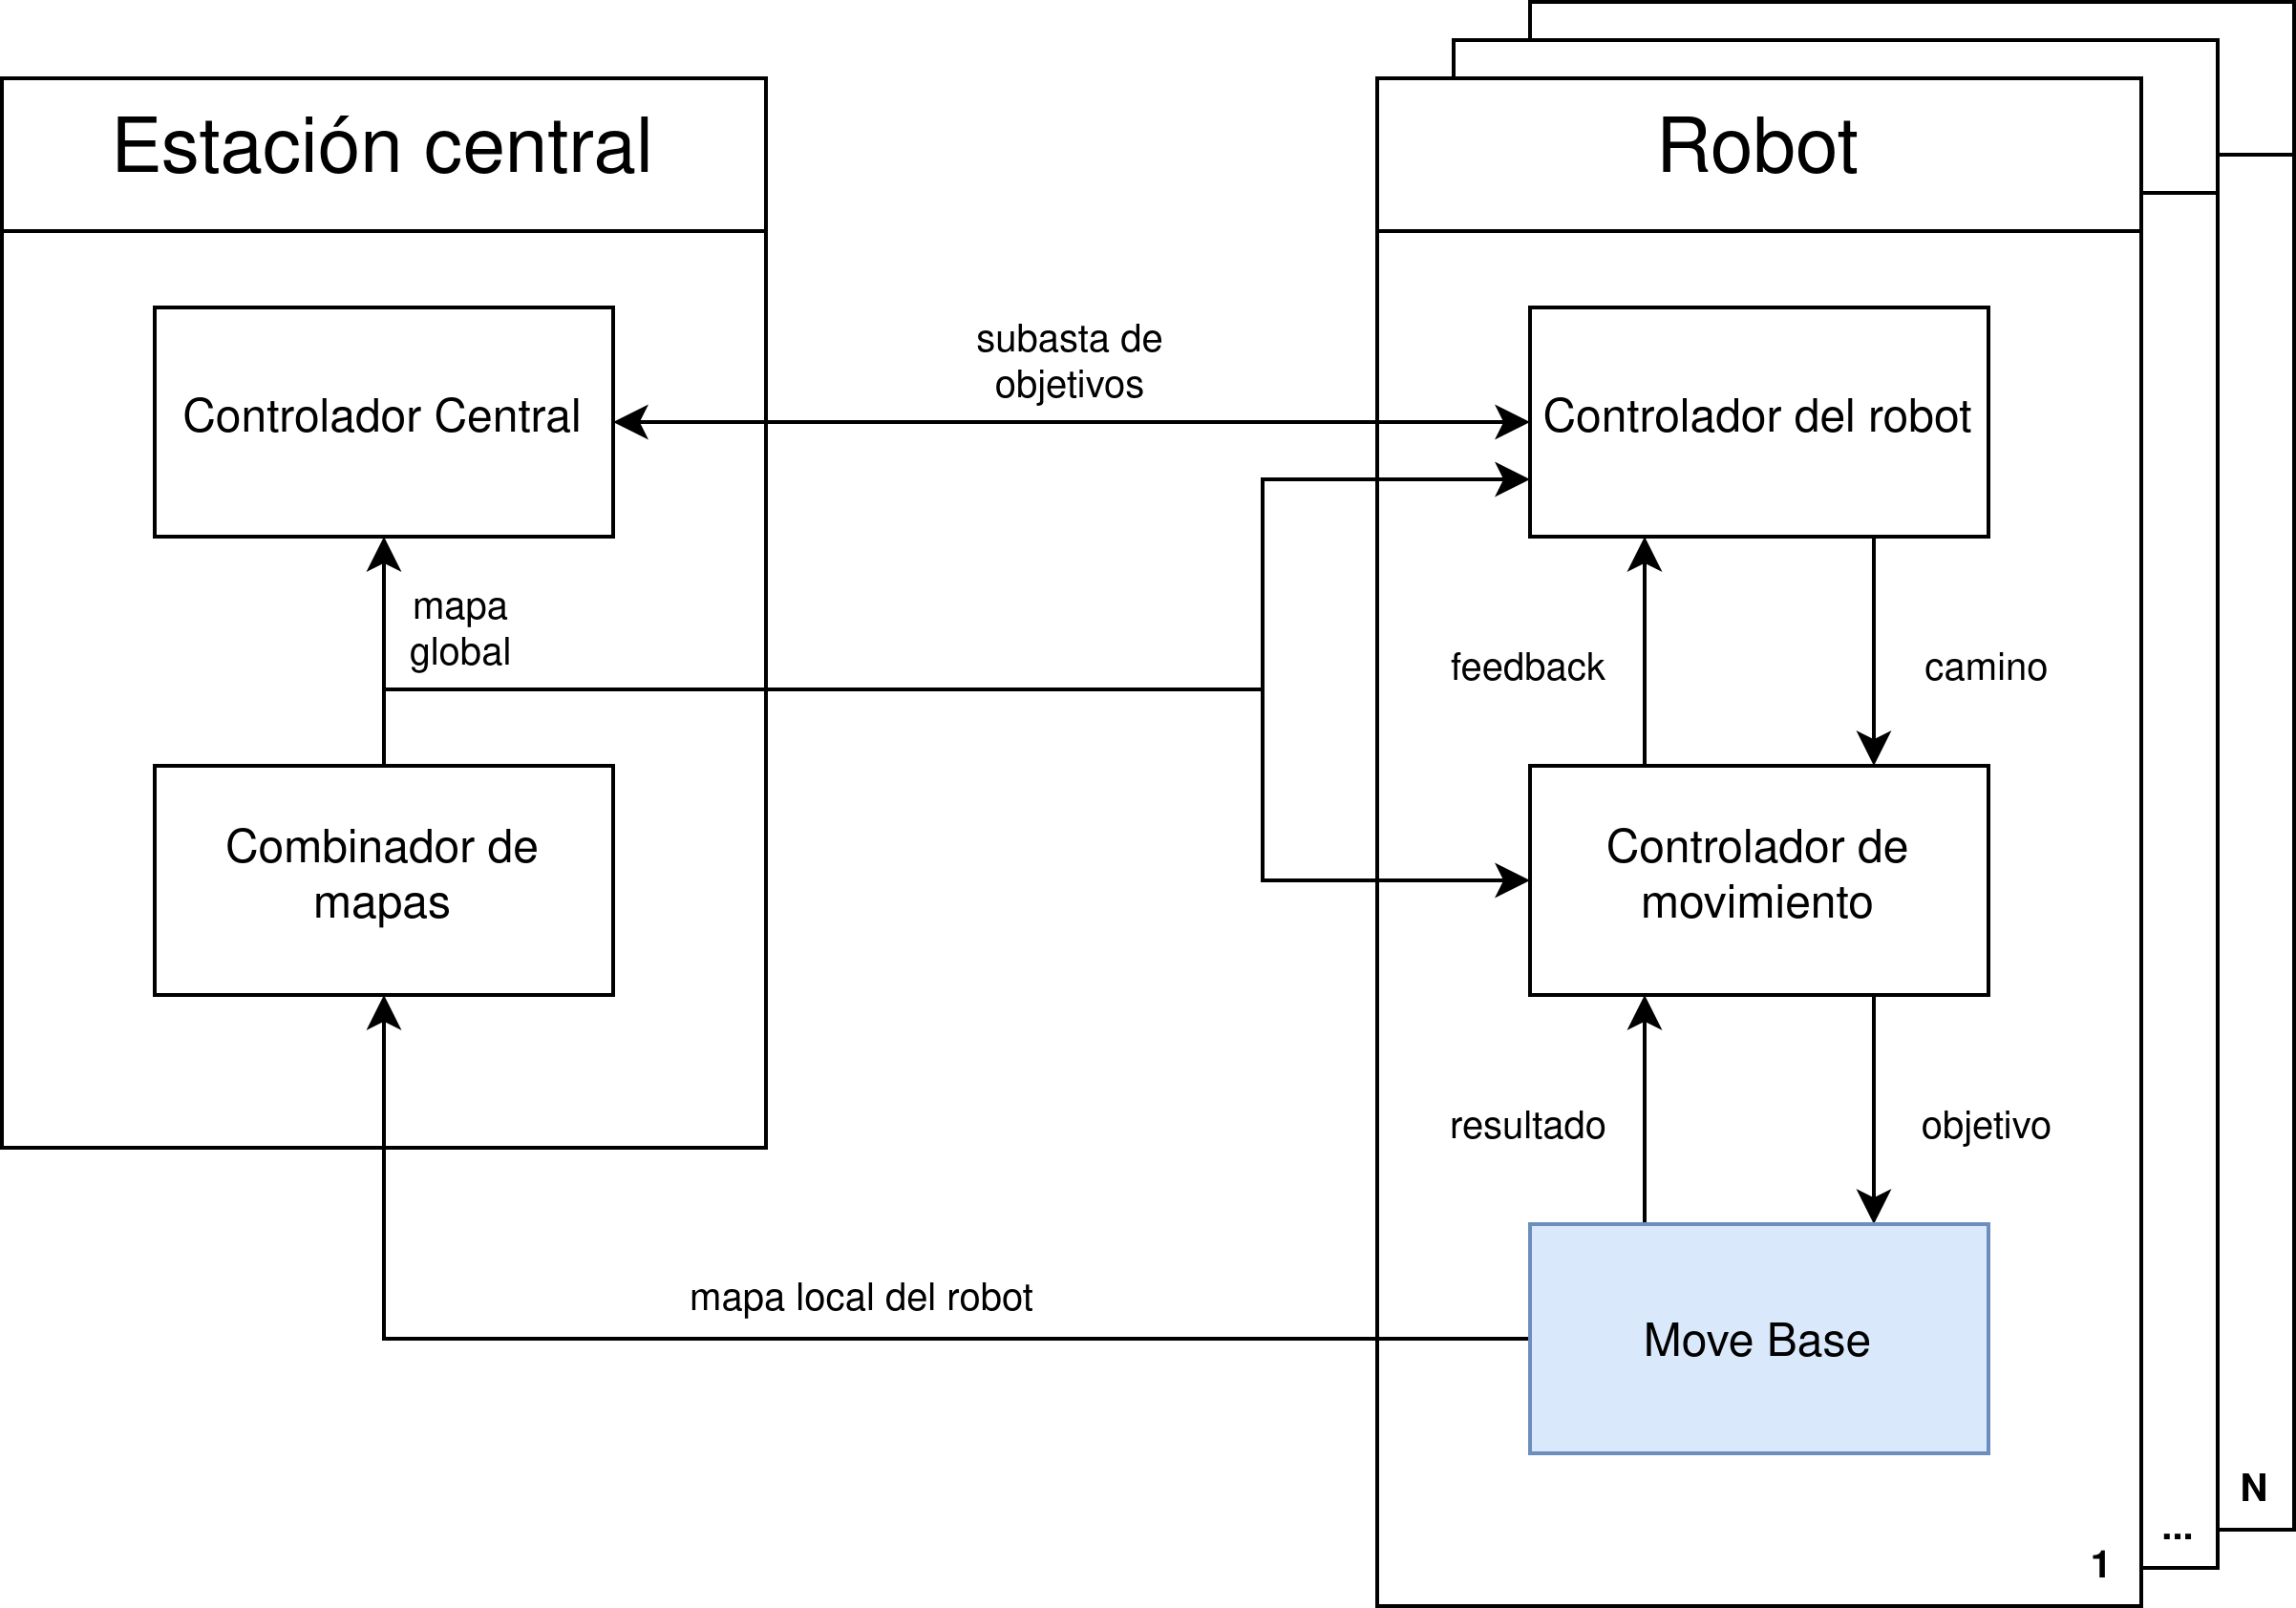
\includegraphics[width=1\linewidth]{imagenes/arquitectura.png}
  \caption[Arquitectura de la solucion propuesta.]{Arquitectura de la solución propuesta. El modulo coloreado con azul es provisto por ROS. Los módulos no coloreados fueron  implementados en esta propuesta.}
  \label{fig:arquitectura}
\end{figure} 

En lo que resta de esta sección se comentará cada modulo, tanto sus tareas y como sus interacciones con el resto de los módulos.

\subsection{Move Base}
El modulo \emph{Move Base} consiste en una instancia del nodo ROS
\emph{move\_base} \cite{ROS-move_base} que provee una interfaz para configurar,
ejecutar y interactuar con el \emph{stack de navegación} de ROS
\cite{ROS-navigation}. 

El stack de navegación de ROS es un conjunto de nodos que tienen como propósito
que un robot pueda navegar el entorno hacia objetivos dentro del mismo. En la
figura \ref{fig:move_base} se muestra un diagrama que repesenta a los nodos que
componen al stack de navegación de ROS y sus interacciones.

\begin{figure}[H]
  \center
  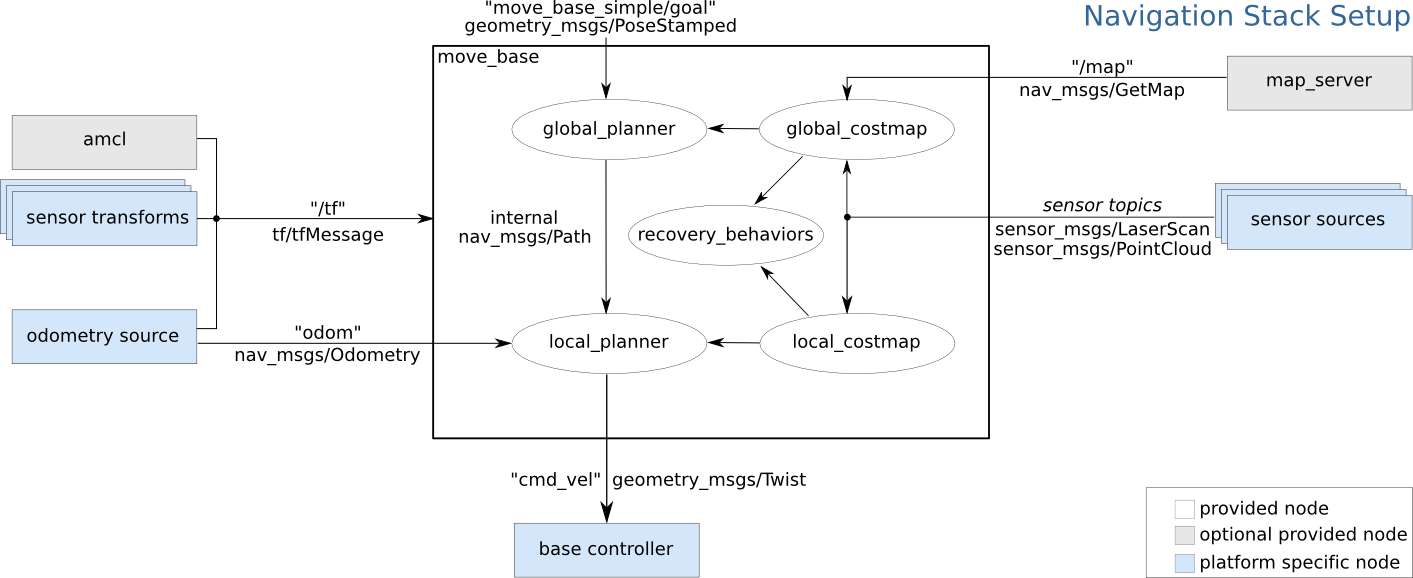
\includegraphics[width=1\linewidth]{imagenes/move_base.png}
  \caption[Arquitectura del stack de navegación de ROS.]{Arquitectura del stack de navegación de ROS. Extraída de \cite{ROS-move_base}.}
  \label{fig:move_base}
\end{figure} 

Cuando se establece un objetivo de navegación este se trasmite al nodo
\emph{global\_planner} este se encarga de generar un plan de alto nivel
consistente de un numero de subobjetivos, que de seguirse en secuencia llevan
al robot al objetivo sin colisiones.

El camino generado por el \emph{global\_planner} es enviado al nodo
\emph{local\_planner} que se encarga de tomar el plan en alto nivel y
traducirlo a la secuencia las velocidades lineales y angulares que un robot
debe tener a lo largo del tiempo para seguir el global. A dicha secuencia de
velocidades se le conoce como plan local.

El stack de navegación permite utilizar distintas implementaciones de
\emph{global\_planner} y \emph{local\_planner}. En el trabajo desarrollado se
hace uso del \emph{global\_planner}\cite{ROS-global_planner} valga la
redundancia llamado \emph{global\_planner} y el \emph{local\_planner} llamado
\emph{teb\_local\_planner}\cite{ROS-teb_local_planner}.

Para generar sus planes tanto \emph{local\_planner} como \emph{global\_planner}
requieren de un mapa, de esto se encargan los nodos \emph{local\_costmap} (mapa
local) y \emph{global\_costmap} (mapa global) respectivamente. Ambos dos son
una instancia de una misma clase de nodo llamada \emph{costmap\_2d}
\cite{ROS-costmap_2d}, que dentro de sus funcionalidades esta la de de
construir una grilla de ocupación a partir de los datos sensoriales provistos
por los robots. Las principales diferencias entre el mapa global y el local son su
tamaño de celda (pequeño en el local y grande en el global), sus dimensiones
del mapa (el mapa global es el mapa completo mientras que el local es solo una
porción) y sus marcos de referencia (el mapa global suele estar fijo, el local se
centra en el robot).

El nodo \emph{recovery\_behaviors} permite ejecutar comportamientos de
recuperación de detectarse que el robot no esta avanzando de forma correcta al
objetivo. Para la solucion desarrollada solo se hace uso del comportamientos de
recuperación que consite en que el robot rote en el lugar.
%en el lugar y forzar que recalculen porciones del mapa.

% El \emph{global\_planner} hace uso de un mapa global, este mapa es provisto por 


% lograr esto cuando se establece un objetivo de navegación,


% de permitir que un robot pueda mover que a partir de información sobre la ubicación, sensores del robot, v 


\subsection{Combinador de mapas}
El modulo \emph{Combinador de mapas} es el encargado de mantener el mapa del entorno
explorado. Este recibe las actualizaciónes de los mapas globales que son
generados por el nodo \emph{global\_costmap} del stack de navegacion de cada
robot y las combina en un unico mapa que contenga toda la información
recopilada del entorno. Cuando el mapa combinado global se actualiza este
retrasmite lo actualizado a diversos componentes del sistema (ver figura
\ref{fig:arquitectura}) que utlizan el mapa del entorno explorado para llevar a
cabo alguna de sus tareas. 

\subsection{Controlador central}

El modulo \emph{Controlador central} lleva a cabo la identificacion de objetivos, es decir detectar en
el mapa actual los potenciales objetivos de exploracion. 

A su vez es el principal responsable de realizar la asignacion de objetivos.
Específicamente la asignacion de objetivos consiste en una subasta en la cual
este modulo actua como subastador. La subasta se puede resumir de la siguiente
manera, los objetivos de exploracion identificados son transmitidos desde el
\emph{controlador central} a los robots los cuales valuan a dichos objetivos segun que
tan conveniente les es llegar a ellos. Los robots envian sus valuaciones a la
central la cual aplica una algorimo para determinar que objetivo le corresponde
a cada robot y posteriormente le informa a cada robot que objetivo le
corresponde.

% tiene el
% siguiente funciona en la cual  de objetivos consite en tomar los objetivos
% identificados y coordinar

% La prinicpal es la de llevar a cabo la identificación de tareas y ser el 

% e encarga de coordinar las subastas de segmentos, es decir, genera la
% información necesaria para esta, decide cuando comienza la subasta y cuando
% termina el plazo para ofertar, computa los resultados y se encarga de las
% comunicaciones necesarias para llevarla a cabo.

\subsection{Controlador de movimiento}
El modulo \emph{Contrador de movimiento} es como su nombre lo indica el modulo
que se encarga de controlar el movimiento del robot. Específicamente recibe
caminos compuesto por celdas de la grilla de ocupacion que en secuencia llevan
a un objetivo de exploracion, y se encarga de ir enviando objetivos de
navegacion al modulo \emph{Move Base} para que el camino sea ejecutado de forma
rapida evitando maniobras innecesarias.

Tambien lleva a cabo una capa superior de comportamientos de recuperacion
extendiendo los provistos por el modulo \emph{Move Base}.

Indica al \emph{Controlador del robot} si se completo el camino con exito, o
existe algun problema.

\subsection{Controlador del robot}
El \emph{Controlador del robot} es el modulo que se encarga de valuar los
objetivos cuando ocurre una subasta. A su vez se encarga de procesar las
asignaciones de objetivos determinadno el camino que lleva al objetivo y
enviandolo al modulo \emph{Controlador de movimiento}. 

Tambien es responsable por solicitar el inicio de una subasta al
\emph{Controlado central} cuando el \emph{Controlador de moviemiento} indica el
exito o el fracaso en seguir el camino asignado.

% Tambien pide la subasta.\todo{explicar mejor}

% \section{Ciclo de robot}

% \section{Ciclo de la central}
\section{Definiciones}
\subsection{Grillas de ocupacion}
En el contexto de este trabajo se utlizara las siguientes definiciones referentes a
grillas de ocupacion, introducidas en la seccion \ref{subsec:mapas}.

El conjunto $C\subseteq R^2$ esta conformado de los centros de cada celda de la
grilla de ocupacion. Las celdas se repreresentan segun sus centros y viceversa
sin ambigüedad, por lo tanto en lo que resta de este informe se usaran ambos
terminos de forma indistinta.

Se dice que cada celda $c\in C$ tiene asociada una probabilidad $P(c|m(1:k))$
de estar ocupada, donde $m(1:k)$ es el conjunto de medidas resultantes de algun
sensor desde el comienzo de la exploarcion.

La funcion $e : C \rightarrow E$ dado un centro de celda, devuelve uno de los
tres estados posibles $E=\{libre, ocupado, desconocido\}$ segun la probabilidad
asociada a $c$. En el contexto de este proyecto la funcion $e$ se define segun
(\ref{eq:estado}).
\begin{equation} 
  e(c)= 
  \left \{ 
    \begin{aligned}
       libre       &\ \ \ \text{ si}& P(c|m(1:k)) < 0.5 \\
       desconocido &\ \ \ \text{ si}& P(c|m(1:k)) = 0.5 \\
       ocupado     &\ \ \ \text{ si}& P(c|m(1:k)) > 0.5
    \end{aligned}
  \right .
  \label{eq:estado}
\end{equation}

La funcion $ady : C \rightarrow P(C)$ dada una celda devuelve el conjunto de
celdas adyacentes a la misma. La definicion de $ady$ utlizada en el contexto de
este proyecto se presenta en (\ref{eq:vecinos}) donde $n_1, n_2, ..., n_8$ se
corresponden a vecinos diagonales y horizontales de $c$ segun se muestran en la
figura \ref{fig:vecinos}.

\begin{equation} 
 ady(c)=\{n_i : 1\leq i \leq 8, n_i \in C\}
 \label{eq:vecinos}
\end{equation} 

\begin{figure}[H]
  \center
  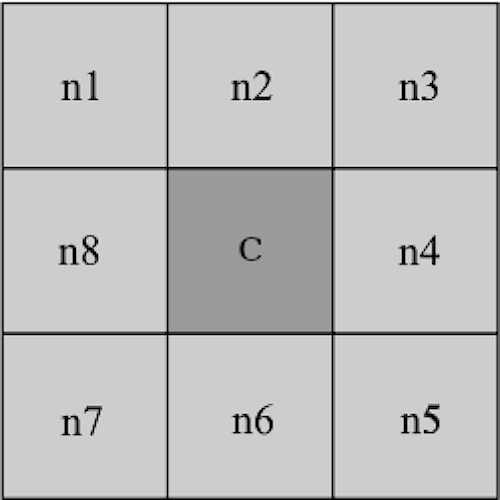
\includegraphics[width=0.3\linewidth]{imagenes/vecinosSharp.png}
  \caption[Vecinos de una celda en una grilla de ocupación.]{Vecinos de una celda en una grilla de ocupación.}
  \label{fig:vecinos}
\end{figure} 

Notar que la relacion de adyacencia es simetrica por lo que $c_1 \in ady(c_2) \Leftrightarrow c_2 \in ady(c_1)$.
% This map is obtained from the occupancy probability grid by a simple clipping operation with a threshold of 0.5. The gray areas of the maximum-likelihood map correspond to cells that have not been sensed by the robot.

\subsection{Componentes conexas} \label{subsec:CompComp}
Una descomposicion en componentes conexas de un conjunto de
celdas $C$ es un conjunto $CC\in P(C)$ compuesto por $N$ conjuntos $C_i$ con
$i\in[1,N]$ tales que:
\begin{itemize}
  \item $\bigcup_{i=1}^{N}C_i = C$ 
  \item Para todo $i,j \in [1,N]$ $C_i\cap C_j = \emptyset$
  \item Para todo $i \in [1,N]$, para todo par $c_1,c_2 \in C_i$ se cumple que $c_1 \in ady(c_2)$.\todo{arrglar, seria hay camnio en $C_i$}
  \item No existen $i,j \in [1,N]$ tales que existan $c_1 \in C_i$ y $c_2 \in C_j$ que cumplan con $c_1 \in ady(c_2)$ 
\end{itemize}

Un ejemplo de una descomposicion en componentes conexas se muestra en la figura \ref{fig:fronterasCompCon}.

\begin{figure}[H]
  \centering
  \subfloat[Las celdas pertenecientes a $C$ se marcan con azul.]{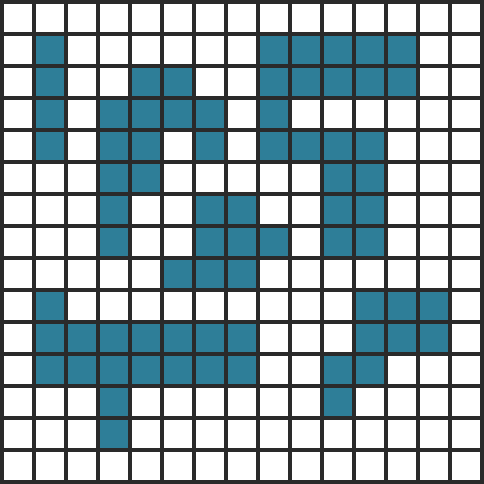
\includegraphics[clip=true, width=0.40\linewidth]{imagenes/compCon/a.png}}
  \qquad
  \subfloat[Cada componente conexa de $C$ se contornea con rojo.]{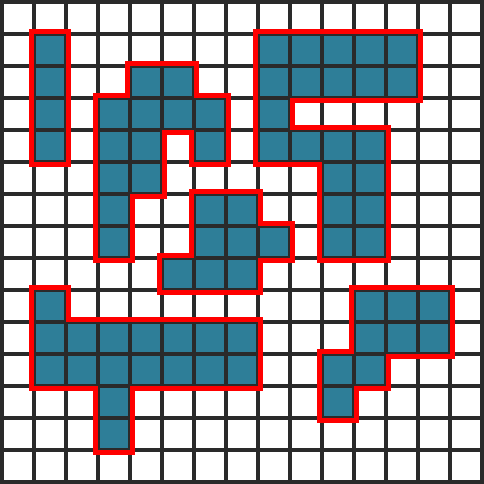
\includegraphics[clip=true, width=0.40\linewidth]{imagenes/compCon/b2.png}}

  \caption{Descompocicion en componentes conexas.}\label{fig:descCompCon}
\end{figure}

Es posible obtener las compnentes conexas de un conjunto cualquiera de
celdas $C$ con el algoritmo \ref{alg:compcon}.

\begin{algorithm}[H]
\SetAlgoLined
  \SetKwInOut{Input}{Entrada}
  \Input{$C$}
  $restantes := C$ \\
  $CC := \emptyset$ \\
  $pila :=$ Pila vacia \\
  $i := 1$ \\
  \While{ $\neg restantes.vacia()$ } {
    $C_i := \emptyset $ \\
    $c :=$ elemento arbitrario de $Restantes$ \\

    % \tcp{DFS desde $c$ agregando las celdas visitadas a la componente conexa $C_i$}

    $C_i :=  C_i \cup \{c\}$ \\
    $restantes := restantes - \{c\}$ \\
    $pila.apilar(c)$ \\
    \While { $\neg pila.vacia()$ } {
      $c := pila.desapilar()$ \\
      \For{ $cA \in ady(c)$ } {
        \If{ $cA \in restantes$ } {
          $C_i :=  C_i \cup \{c\}$ \\
          $restantes := restantes - \{c\}$ \\
          $pila.apilar(c)$ \\
        }
      }
    }
    $CC := CC \cup C_i$ \\
    $i := i + 1$ \\
  }
  \Return $CC$ 

  \caption{Descomposicion en componentes conexas de $C$}
  \label{alg:compcon}
\end{algorithm}

Este algoritmo se resume en elegir una celda $c\in C$ que no este aun en una
componente conexa (linea 6), aplicar un \emph{depth-first search} (DFS)
partiendo $c$ agregado todas las celdas recorridas a una misma componente
conexa (lineas 7-19). Repetir dicho procedimiento hasta que todas las celdas
pertenezcan a alguna componente conexa (linea 4). Este algormitmo es analogo al
que esta presente en \cite{hopcroft1973algorithm}.

\section{Identificación de objetivos}
El problema de identificación de objetivos consiste en determinar los puntos
del espacio a los cuales es conveniente enviar robots para recolectar nueva
informacion sobre el entorno explorado. Estos puntos son los llamdos objetivos
de exploración (seccion \ref{sec:exploracion}). 
% En el contexto del trabajo desarrollado al utlizarse una grilla de ocupacion
% como mapa los 
% se hablara de celdas en lugar de puntos, existiendo una correspondencia entre
% cada celda y un unico punto en el espacio, su centro.

\subsection{Fronteras}
En \cite{yamauchi1998frontier} se propone que los lugares que permiten
recolectar la mayor cantidad de nueva informacion sobre el entorno son las
fronteras entre el espacio conocido y desconocido. Y que por lo tanto dichas
fornteras deben ser los objetivos de exploración.
Al utlizar una grilla de ocupacion como mapa, las fronteras se definen como las
celdas cuyo estado asociado es $libre$ y son adyacentes a una celda cuyo estado
asociado es $desconocido$ (figura \ref{fig:fronteras}).
Por lo tanto segun Yamauchi los objetivos de exploración seran las celdas
fronteras $F$ segun se definen en (\ref{eq:fronteras}).
\begin{equation} 
  F = \{ c \in C : e(c) = libre, \exists n \in ady(c), e(n) = desconocido  \}
  \label{eq:fronteras}
\end{equation}

\subsection{Simplificacion de Fronteras basada en K-Means}
En \cite{amorin2019novel} se argumenta que tratar todas las celdas fronteras
como objetivos de exploración diferentes podría ser computacionalmente
prohibitivo. Por lo tanto, para reducir el costo computacional, se intenta
reducir los objetivos de exploración a las celdas frontera mas representativas,
a las cuales se denominaran como fronteras significativas.

Para determinar las fronteras significativas, primero, las celdas fronteras $F$
se descomponen en sus componentes conexas $\mli{FC}=\{F_1,F_2,...F_N\}$
(seccion \ref{subsec:CompComp}), un ejemplo de este tipo de descomposicion se
puede ver en la figura \ref{fig:fronterasCompCon}.

Luego se determinan las fronteras significativas $\mli{FS}_i$ de cada
componente conexa $F_i\in \mli{FC}$. Esto se hace agrupando las fronteras de
$F_i$ con el algoritmo K-Means \cite{macqueen1967some}, y determinando una
frontera significativa por cada una de las $k$ agrupaciones, la
frontera mas cercana de $F_i$ al centroide de la agrupacion (una arbitraria de
las mas cercanas en el caso de que exista mas de una). Un ejemplo de las
fronteras significativas  $\mli{FS} = \bigcup_{i=1}^N \mli{FS_i}$ obtenidas con
este metodo se muestra en la figura \ref{fig:fronterasSig}.

El $k$ utilizado para ejecutar K-Means es el minimo que logra que para toda
frontera $f\in F_i$ existe $\mli{fs} \in FS_i$ tal que $d_{\mli{fs}}(f) \leq
rango$ siendo $rango$ el alcance de los sensores del robot. Es decir, el
conjunto de fronteras significativas $\mli{FS}_i \subset F_i$ cumple con que
cada frontera esta dentro del rango del sensado de alguna frontera
significativa, cuando esto se cumple se dice que $\mli{FS}_i$ cubre a $F_i$, o
que $FS_i$ logra el cubrimiento. En la figura \ref{fig:fronterasSigCub} se
puede ver como las fronteras significativas obtenidas $FS$ logran el
cubrimiento, ya que todas los centros de las fronteras $F$ estan contenidos en
las circunferencias de radio $rango$ centradas en las fronteras significativas
$FS$.

Para encontrar el minimo $k$ con las que se logra un $\mli{FS}_i$ que cubra a
$F_i$, se parte con $k=1$, si el resultado no logra cubrir incrementa $k$ y se
repite el proceso.


\begin{figure}[H]
  \centering
  \subfloat[Se identifican las frotneras,  marcadas con amarillo.]{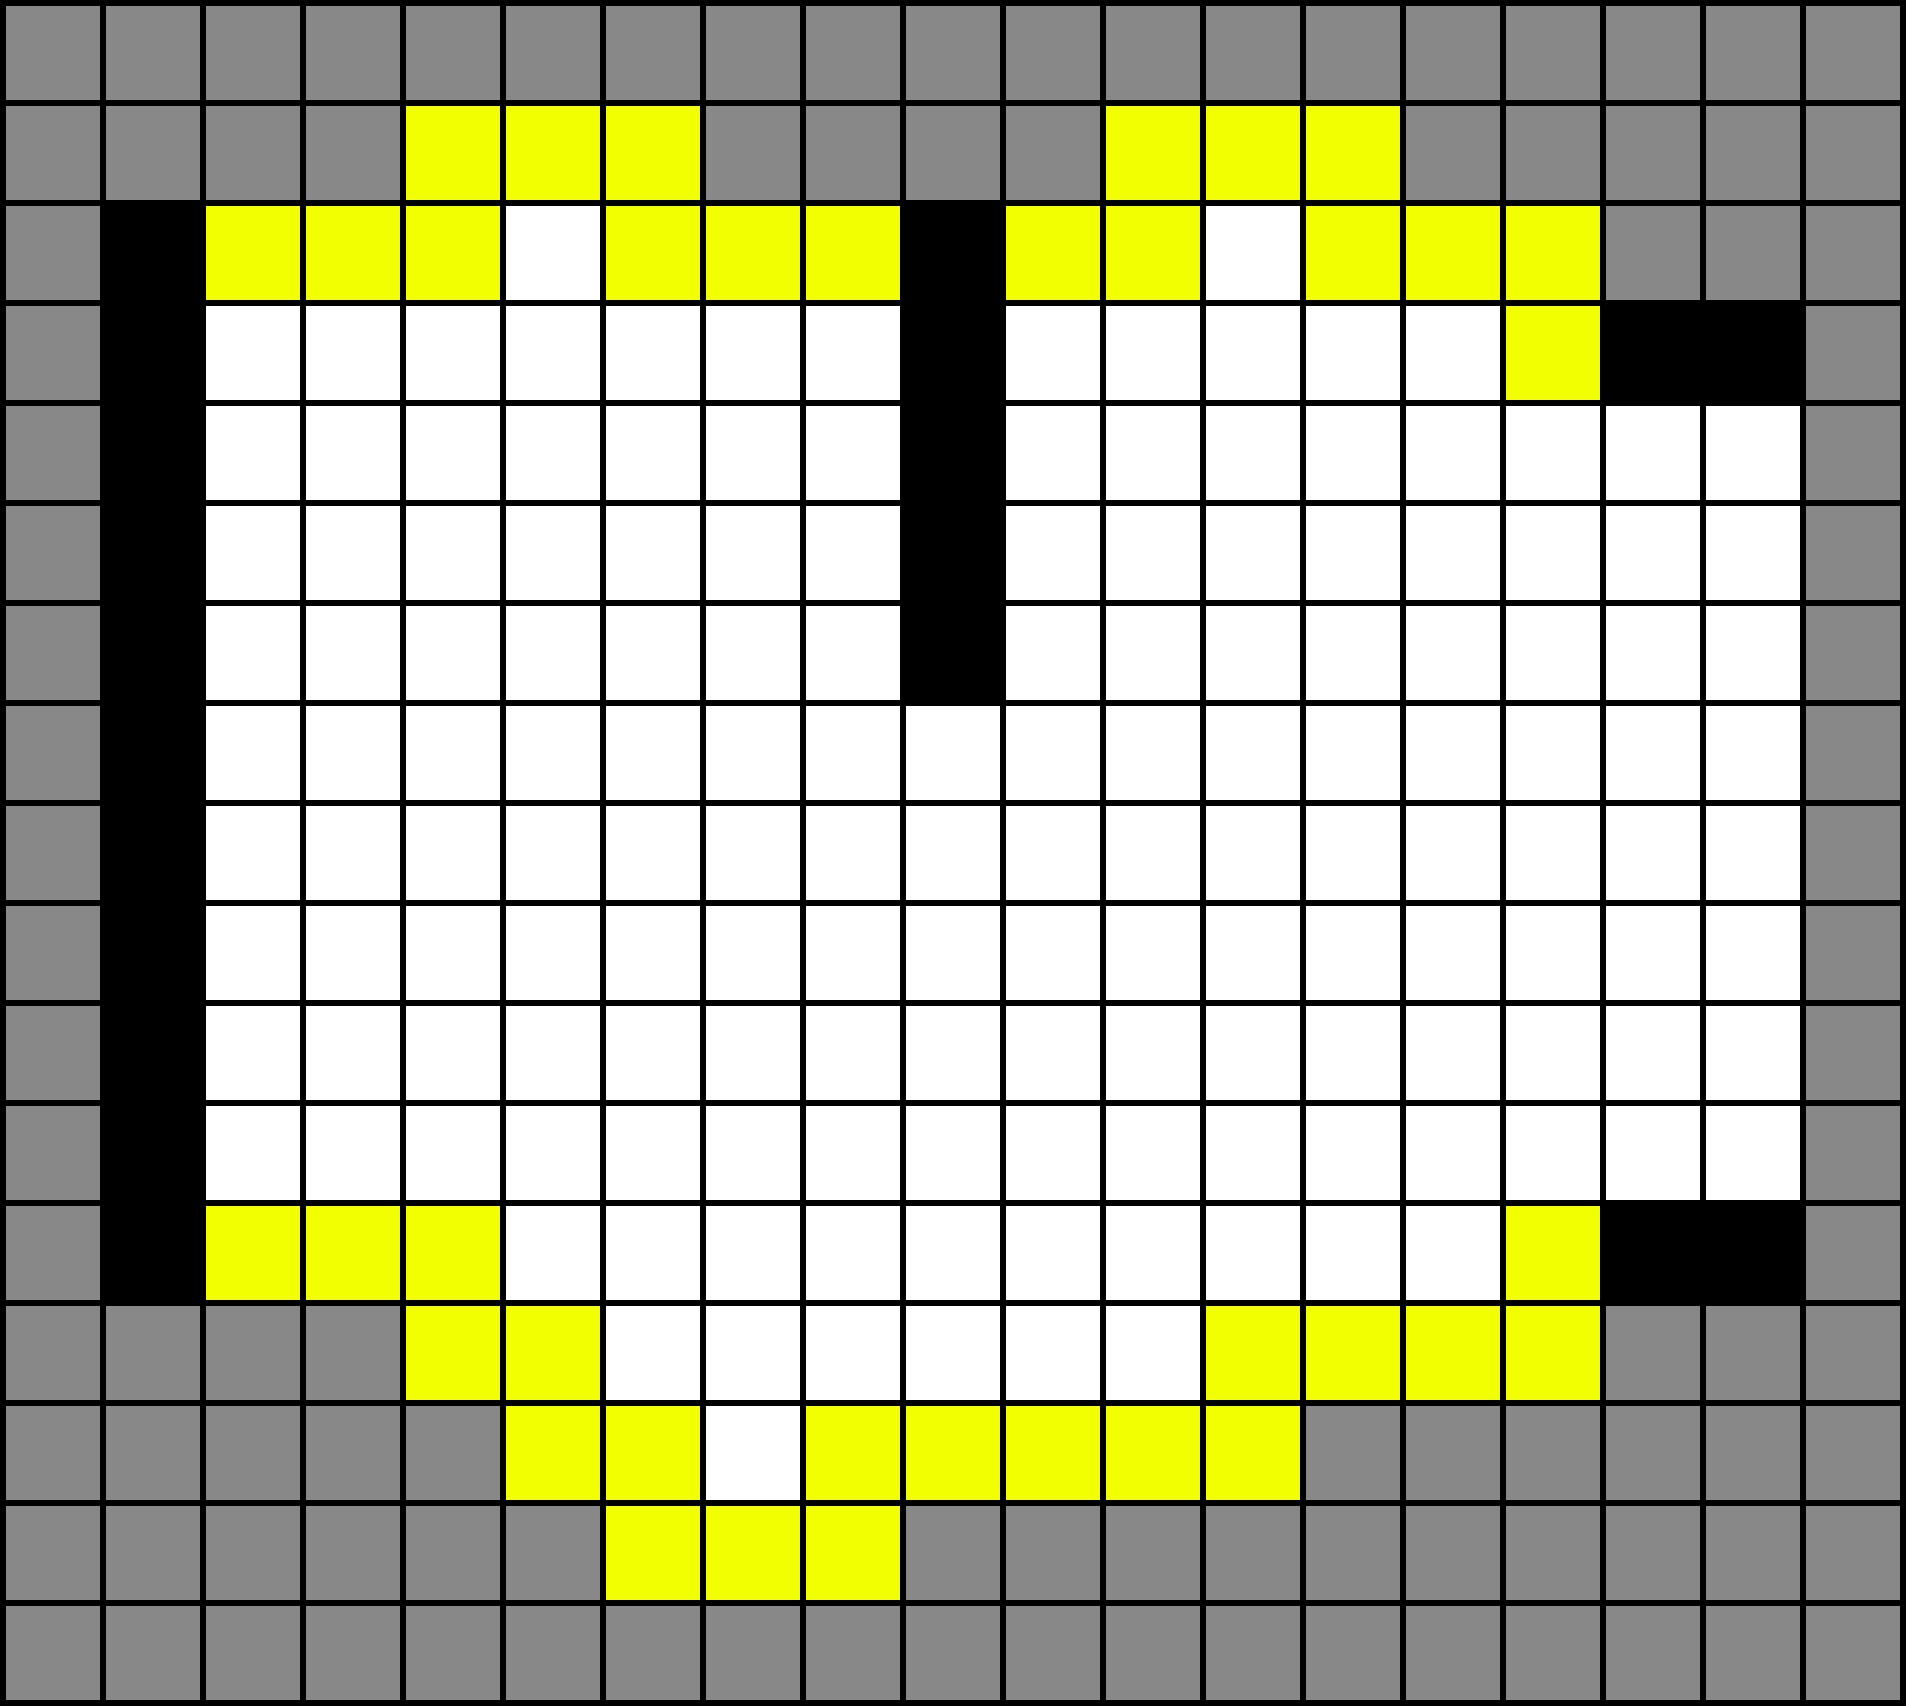
\includegraphics[clip=true, width=0.40\linewidth]{imagenes/fronterasSig/a.png}\label{fig:fronteras}}
  \qquad
  \subfloat[Descompocicion de las fronteras en componentes conexas, cada componente conexa se indica con un color distinto.]{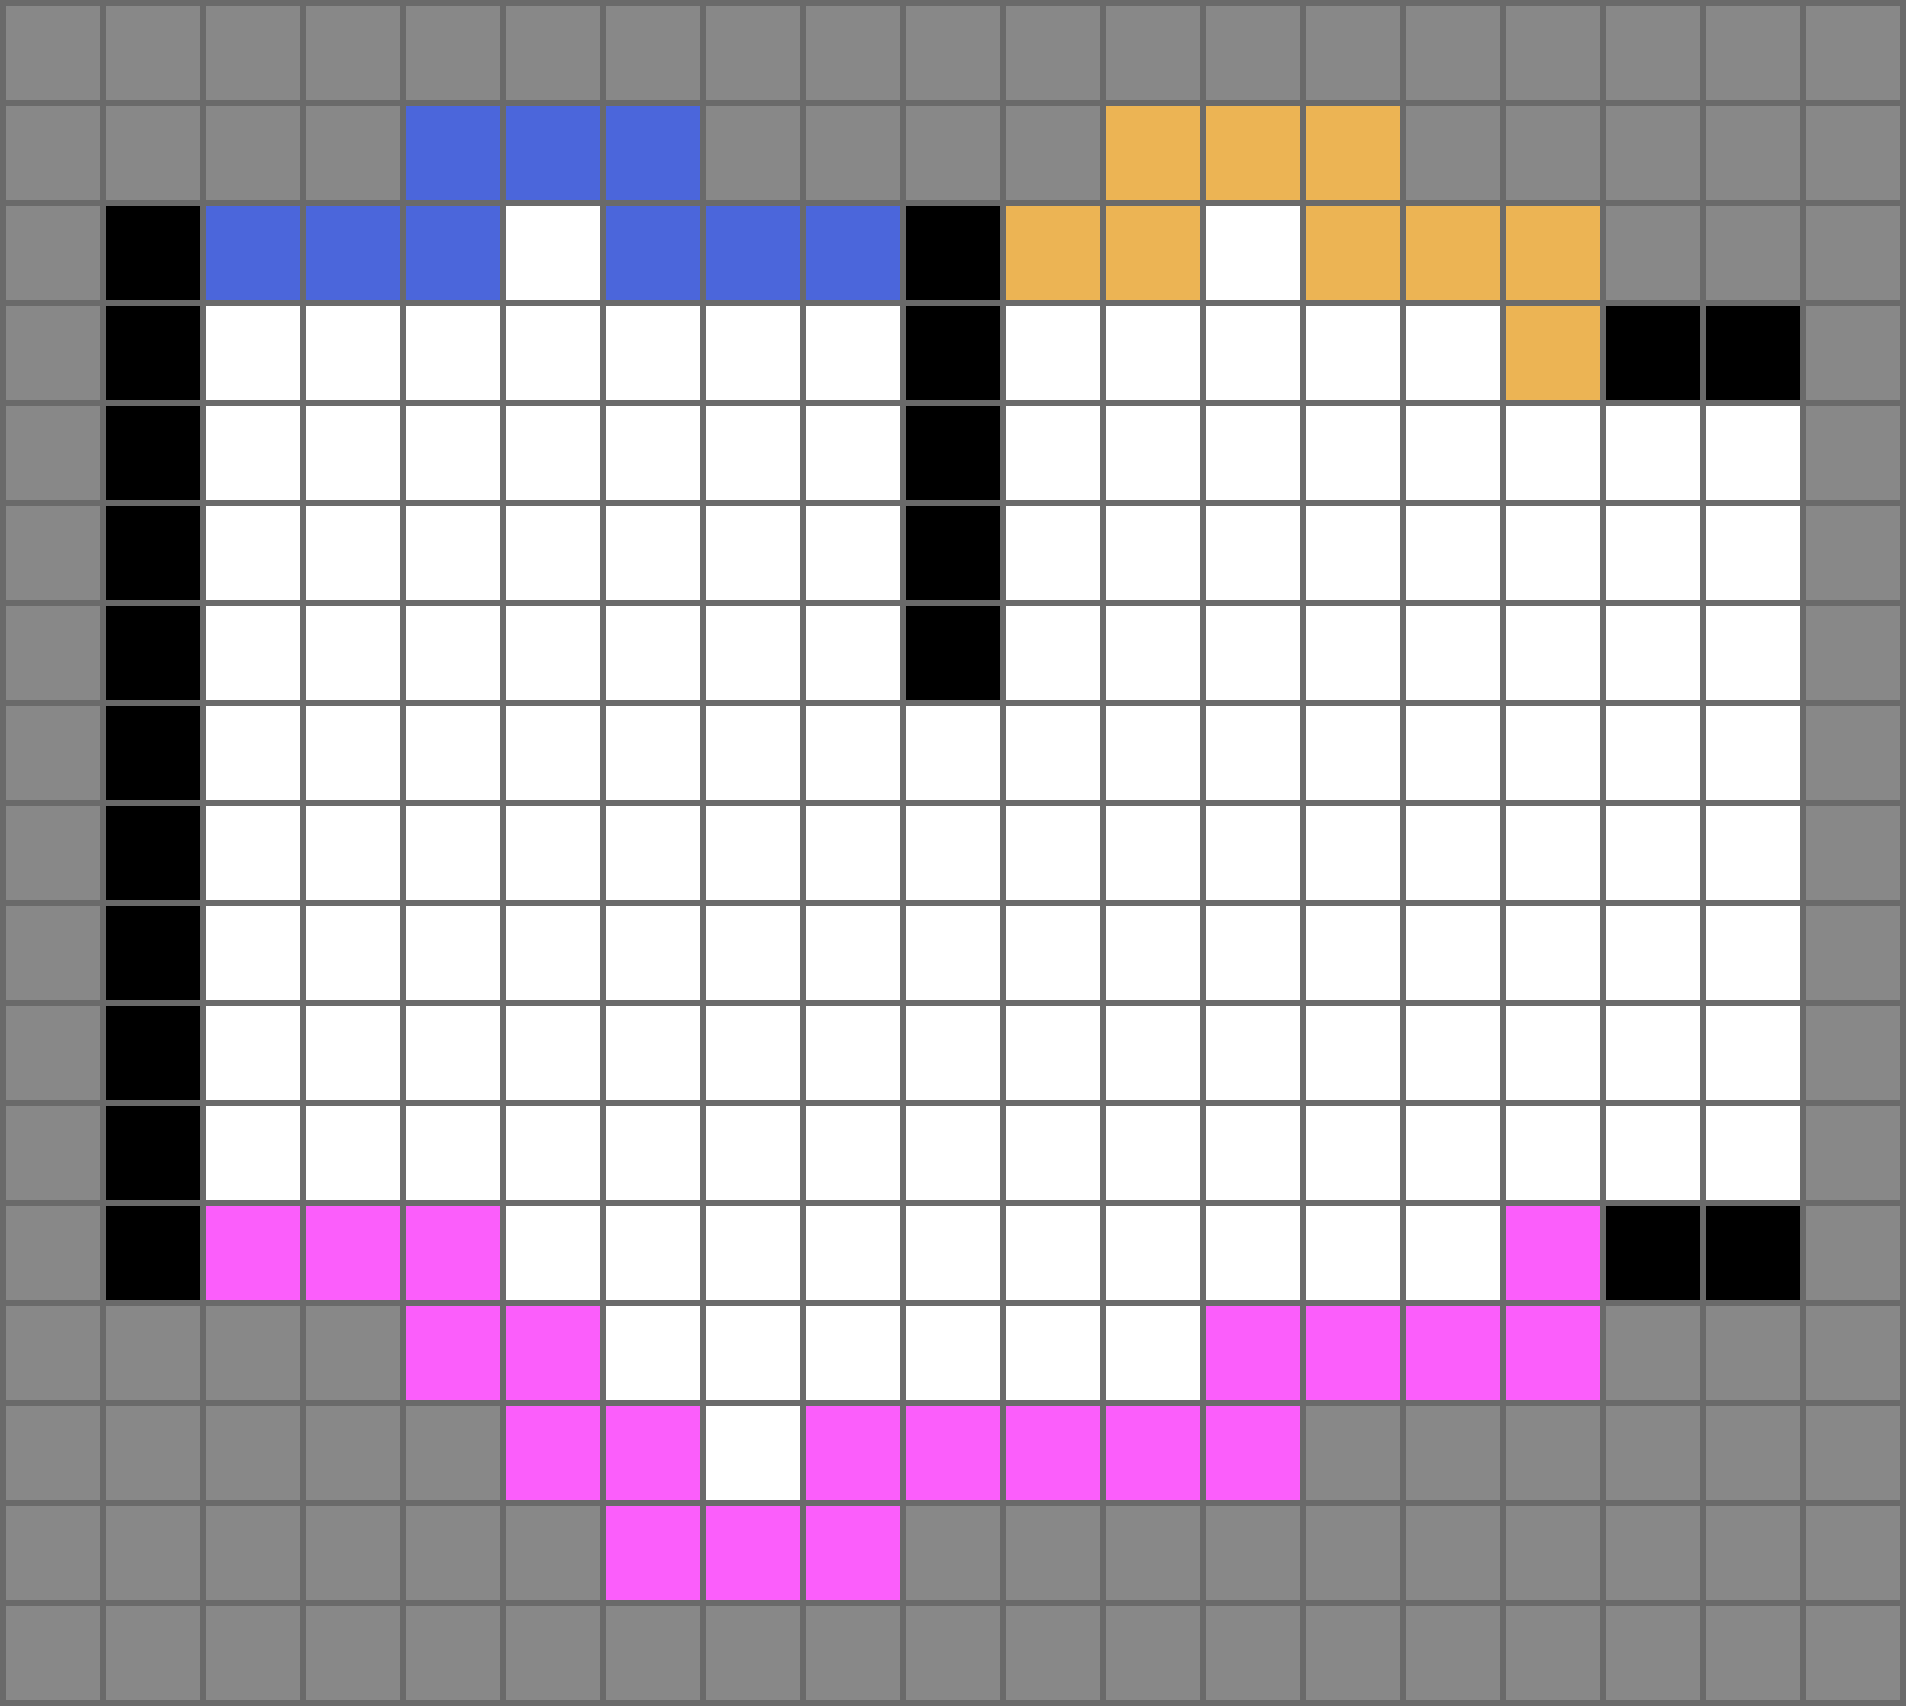
\includegraphics[clip=true, width=0.40\linewidth]{imagenes/fronterasSig/b.png}\label{fig:fronterasCompCon}}
  \qquad
  \subfloat[Fronteras significativas (indicadas con verde) de cada componente conexa.]{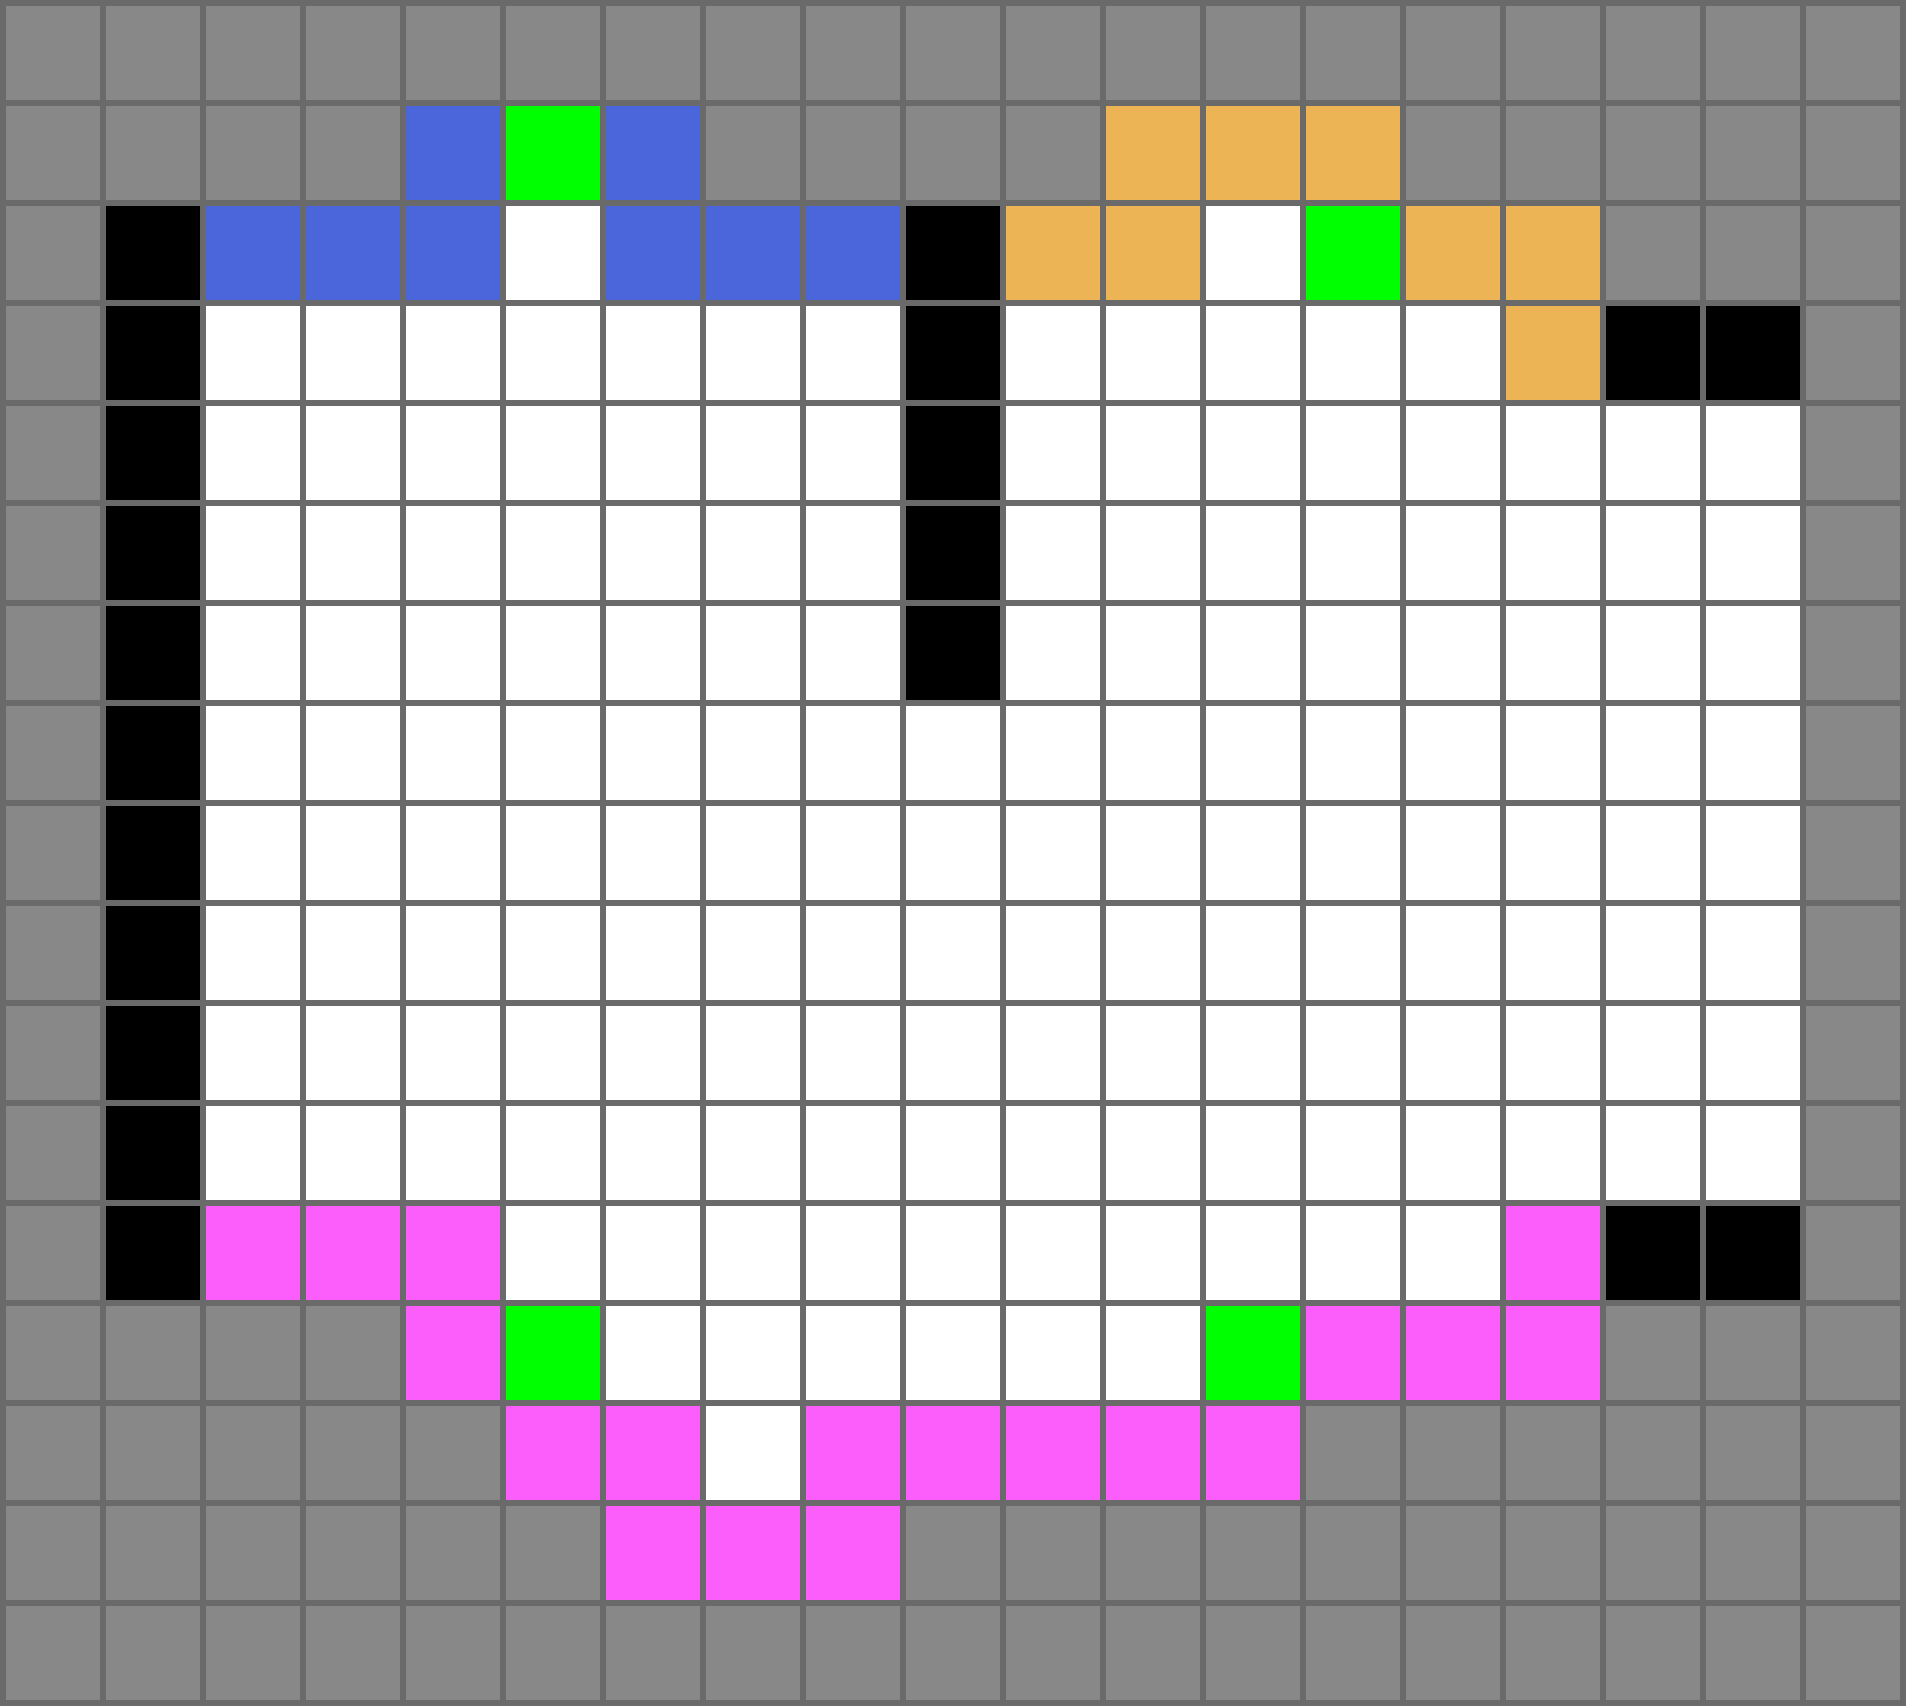
\includegraphics[clip=true, width=0.40\linewidth]{imagenes/fronterasSig/c.png}\label{fig:fronterasSig}}
  \qquad
  \subfloat[Se logra el cubrimiento.]{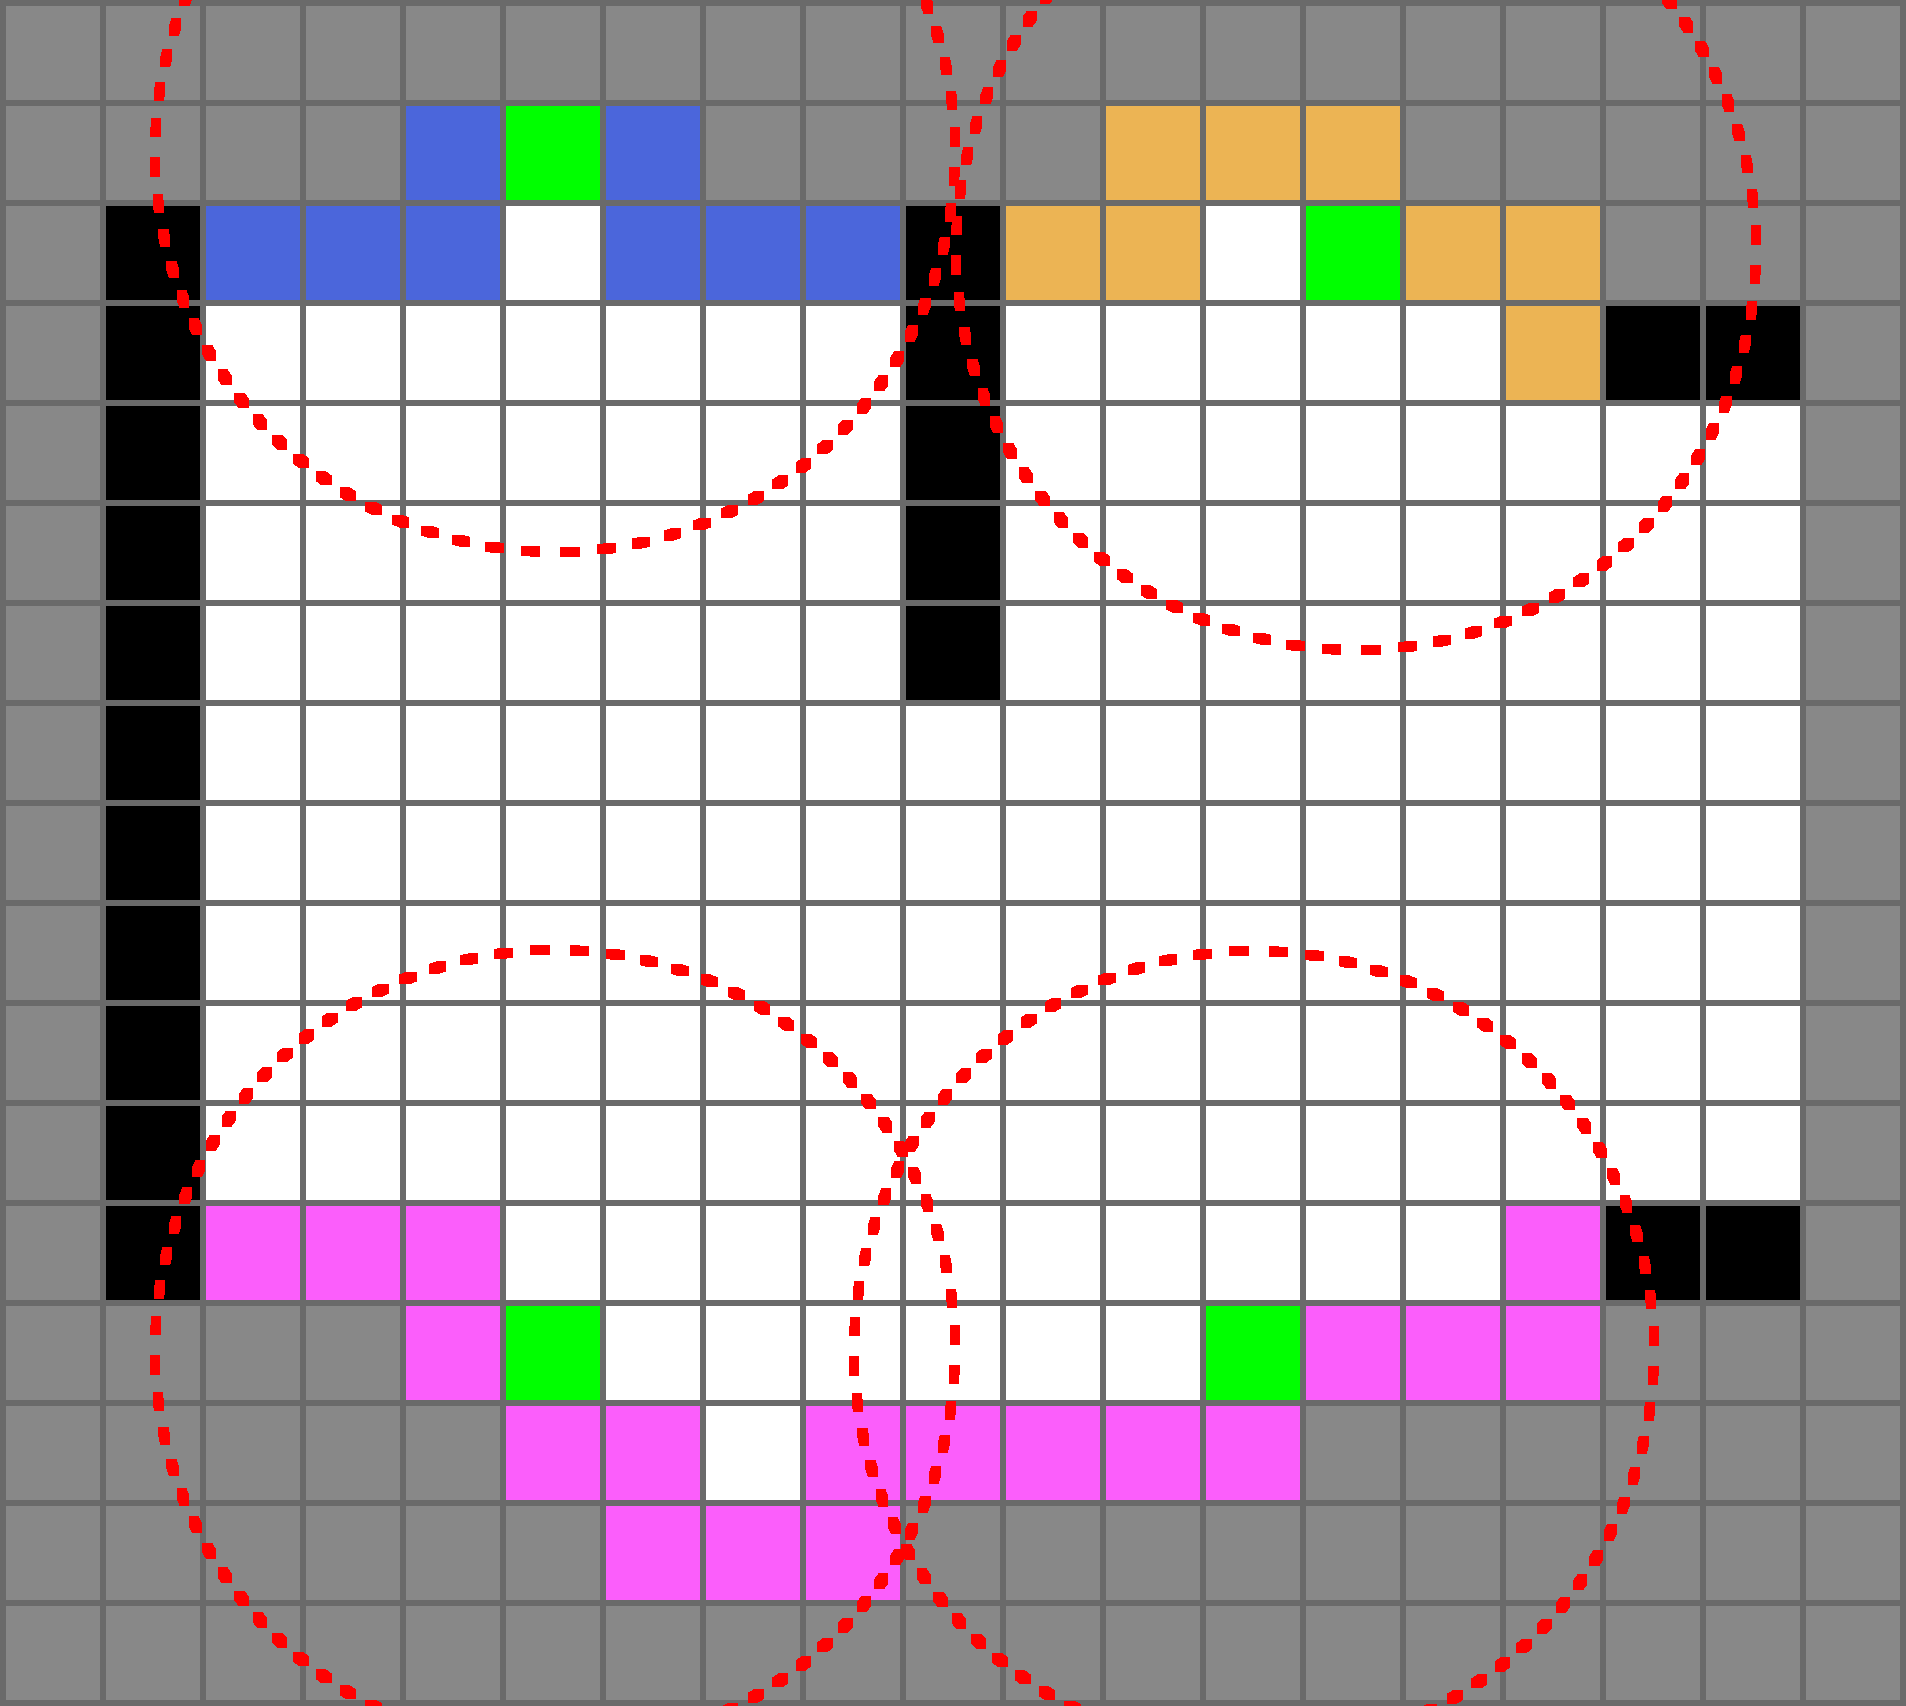
\includegraphics[clip=true, width=0.40\linewidth]{imagenes/fronterasSig/d.png}\label{fig:fronterasSigCub}}

  \caption[Proceso de simplificacion de fronteras según K-Means.]{Proceso de
    simplificacion de fronteras según K-Means. Las circunferencias rojas
    centradas en las fronteas significativas tienen radio $rango=4$ (largos de celda) indicando su
    cubrimiento.
  \cite{Amorin2019}.}\label{fig:ejemploFrontSig}
  % \caption[Proceso de simplificacion de fronteras según K-Means.]{Proceso de simplificacion de fronteras según K-Means. Cada figura corresponde a un mismo entorno parcialmente explorado, representado con una grilla, donde las celdas blancas son libres, las negras ocupadas, y para las grises se desconoce su estado. Basada en figuras de \cite{Amorin2019}.}\label{fig:ejemploFrontSig}
\end{figure}

% En la seccion anterior se presento un metodo que soluciona el siguiente
% problema. Dado un conjunto de  la descomposicion en componentes conexas de
% $F$, $\mli{FC}=\{F_1,F_2,...F_N\}$ se obteniene como salida el conjunto
% $\mli{FS} = \bigcup_{i=1}^N \mli{FS_i}$ que cumple con la restriccion de que
% para todo $i \in [1,N]$ $\mli{FS}_i$ cubre a $F_i$.

El problema descrito hasta el momento se puede resumir en el de  dado un
conjunto de fornteras $F$, obtener un conjunto de fornteras significativas
$\mli{FS}$ que cumplen con la restriccion de que $\mli{FS}$ cubre a $F$.
Recordando que el proposito de usar $\mli{FS}$ como objetivos de exploracion en
lugar de usar $F$ es reducir los objetivos de exploracion entoces es natural
pensar que la soluciones optimas reducen al minimo el $\mli{FS}$ resultante,
mientras mantienen la restriccion de cubrimiento.

% Analizando la restriccion de cubrimiento, se puede ver que un indicador de que
% una solucion es suboptima es que varias celdas $\mli{FS}$ se concentren,
% solapandose las circunferencias de radio $rango$ centradas en ellas. Por
% ejemplo 

Dado esto es posible ver que en el ejemplo presentado en
\ref{fig:ejemploFSKMMal} el resultado obtenido por el metodo presentado en esta
seccion no es optimo ya que existen fronteras significativas innecesarias para
el cubrimiento. 

\begin{figure}[H]
  \centering
  \subfloat[Fronteras significativas obtenidas segun el metodo basado en K-Means.]{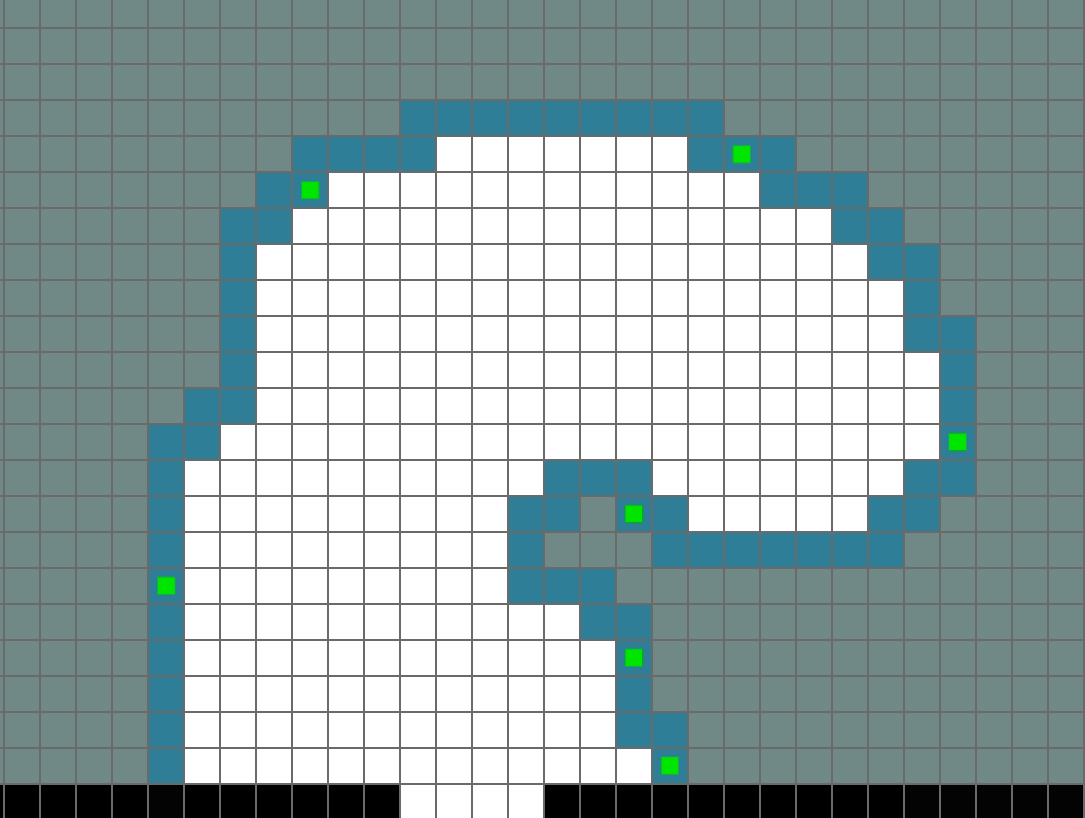
\includegraphics[clip=true, width=0.40\linewidth]{imagenes/fronterasigKMMal/caso1/a_sin_circ.png}}
  \qquad
  \subfloat[Dos de las fronteras significativas de la parte inferior derecha de (a) no son necesarias para lograr el cubrimiento.]{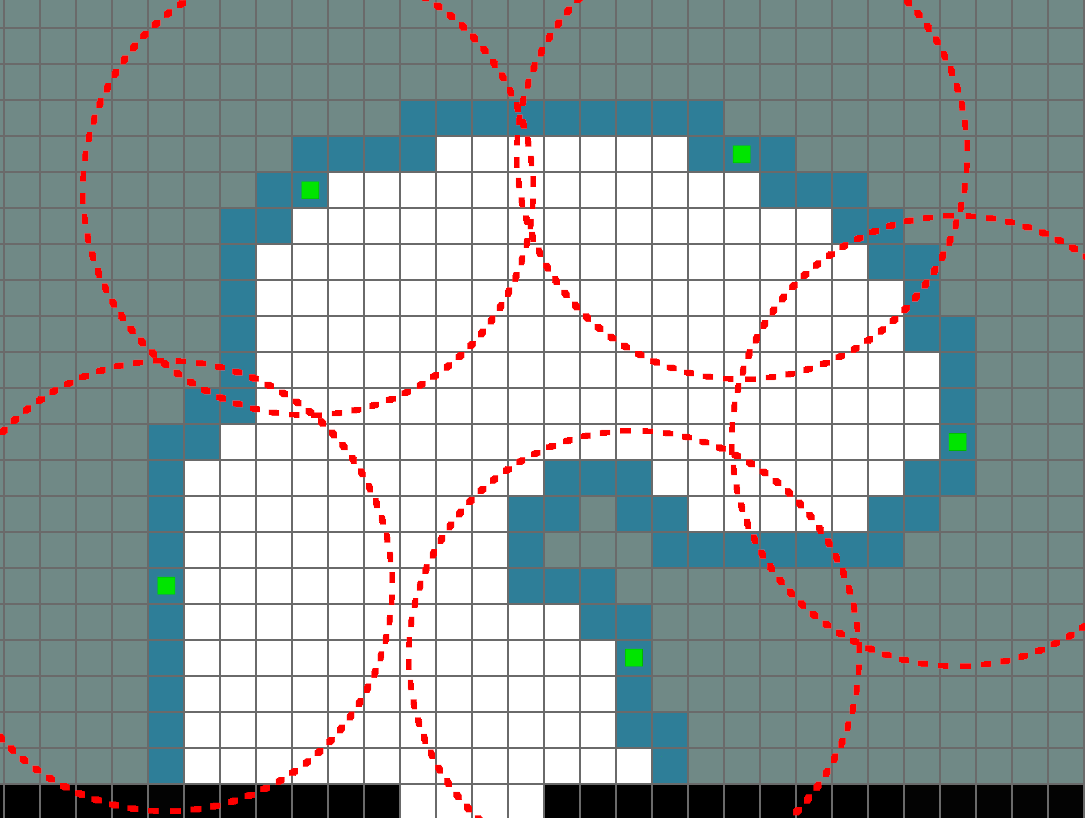
\includegraphics[clip=true, width=0.40\linewidth]{imagenes/fronterasigKMMal/caso1/b.png}}

  \caption[Simplificacion de fronteras suboptima resultante del metodo basado en K-Means.]{Simplificacion de fronteras suboptima resultante del metodo basado en K-Means. Las fronteras de $F_i$ se indican con azul, las fornteras significativas con verde y las
    circunferencias rojas centradas en estas tienen radio $rango=5.6$ (largos de celda) indicando su
    cubrimiento. Extraída de implementacion desarrollada\footnotemark.}\label{fig:ejemploFSKMMal}
\end{figure}
\footnotetext{Podria indicar el bag y el seg}

Resultados suboptimos similares se experimentan de forma consistente %al aplicarse la simplficacion 
sobre componentes conexas con forma serpenteante\todo{no se si este termino se entiende, me es dificil explicarlo bien, con forma de S?},
asimetricas y lo suficientemente extensas como para requerir mas de 4
fornteras significativas para su cubrimiento, 
%con un largo mayor a $rango*8$ 
% \todo[inline]{se entiende la idea del largo aplicada a esto? Creo que puede
% quedar claro mirando la foto pero tengo mis dudas. La idea en realidad seria
% decir que la solucion no es lo suficientemente simple, por ejemplo si con 1
% sola frontera sig ya se cubre todo entonces no va haber problema sin importar
% que tan serpenteante o asimetrica sea. Se me ocurre que puedo tratar la simpleza hablando por el largo puede
% quedar mas claro o mas oscuro, es decir por que 8? fue para poner un valor
% similar al de la foto que necesita 5 fronteras para cubrir }
empeorando (mayor cantidad de fornteras significativas
innecesarias para el cubrimiento) a medida que las componentes conexas de
fronteras son mas extensas y las curvas son mas intrincadas.

% (comentarlos, distribuciones desparejas, acumulacion, no
% equidistantes) 

% Una explicacion posible a este comportamiento es que la distibucion de centroides en K-Means 

% Algo que se repite en estas situaciones es que suele haber zonas, en donde las
% fornteras significativas se acumulan, y zonas en las que estan muy dispersas
% (casi a $rango$ de distancia una de la otra, el maximo). Esto lleva a pensar que K-Means se tiende a ubicar concentrar los centroides en una zona,

Esto se presume que se debe principalmente a dos factores relacionados a
K-Means. (i) K-Means no considera la restriccion de cubrimiento para generar sus
resultados. La restriccion se fuerza ejecutando K-Means con el minimo $k$
(obtenido con prueba y error) segun el cual las fronteras significativas
resultantes logran el cubrimiento. (ii) Los centroides resultantes de K-Means
no son fronteras. Estos se deben traducir a fronteras posteriormente.

% \todo{Hay una arbitrariedad asociada a k-means tambien lo cual puede ser criticado tambien, aunque deberia estudiar mejor el tema, quizas no criticarlo aca pero destacar que el otro metodo es menos opaco en como elige las front sig}
% Esto es la clase de pe la idea de obtener fornteras significativas es reducir el numero
% de objetivos de exploracion,

% El metodo basado en K-Means aunque funciona bien al aplicase en componentes conexas pequeñas, 

% El metodo descrito en la seccion resulta en un conjunto de fronteras
% significativas que cubren a las fronteras, el problema que se detecto
% experimentalmente es que en ciertos casos el resultado  la discribucion de las
% fronteras significativas es mala, se concentran mucho en ciertas porciones y se alejan 

\subsection{Simplificacion de fronteras basada en cubrimiento}\label{subsec:MiSimp}
Con esto en mente se desarrolla un metodo novedoso que considera los dos puntos
destacados anteriormente. (i) Tomando en cuenta el cubrimiento y su
optimizacion como parte fundamental del algorimo. (ii) Dando directamente
fronteras como resultado.

El algorimo al igual que el descrito en la seccion anterior comienza
descomponiendo a las fronteras $F$ en sus componentes conexas
$\mli{FC}=\{F_1,F_2,...F_N\}$ para luego obtener las fronteras significativas
$\mli{FS}_i$ para cada componente $F_i$, siendo el conjunto total de fronteras
significativas $FS = \bigcup^N_{i=0} \mli{FS}_i$

El proceso completo que permite obtener las frontera significativas
$\mli{FS}_i$ para un componente $F_i$ se muestra en el algoritmo
\ref{alg:IdObjGeo}.

\begin{algorithm}[H]
\SetAlgoLined
  \SetKwInOut{Input}{Entrada}
  \Input{$F_i$}

  $\mli{UF} := F_i$ \\
  $\mli{FS}_i := \emptyset$\\

  $\mli{PF} :=$ Cola vacia \\
  \ForEach { $f\in F_i$ } {
    \ForEach{ $\mli{fa} \in ady(f)$ } {
      \If { $e(\mli{fa}) = ocupado$ } {
        $\mli{PF}.encolar(f)$
      }
    }
  }
  \If{$\mli{PF}.vacia()$}{
    $\mli{PF}.encolar($elemento arbitrario de $F_i)$
  }
  \While{$\mli{UF} \neq \emptyset$ } {
    $\mli{pf} := \mli{PF}.desencolar()$\\
    \If{ $\mli{pf} \in \mli{UF}$}{
      $dCen := max \{ d_{\mli{pf}}(\mli{f}) : f\in\mli{UF} \}/2$\\
      $radio := min \{dCentrada, rango\}$\\
      $\mli{FSC} :=\mli{UF} \cap \mathscr{C}(\mli{pf},radio)$\\
      $\mli{fs} := $elemento arbitrario de $\mli{FSC}$\\
      $\mli{FS_i} := \mli{FS_i} \cup \{\mli{fs}\}$\\

      $\mli{RC} := \{ f\in F_i : d_{\mli{fs}}(f) \leq rango\}$\\

      $\mli{UF} := \mli{UF} - \mli{RC}$\\

      \ForEach { $\mli{pf} \in \{ f \in \mli{UF} : \exists c \in \mli{RC}, f \in ady(c)\}$}{
        $\mli{PF}.encolar(\mli{pf})$
      }
    }
  }
  \Return $\mli{FS}_i$ 

  \caption{Simplificacion de fronteras basada en cubrimiento}
  \label{alg:IdObjGeo}
\end{algorithm}

Para obtener las fronteras significativas de $F_i$ el algorimo parte mantiene
las fronteras sigficativas determinadas $\mli{FS}_i$, el conjunto
todas las fronteras que resta cubrir $\mli{UF}$ (siglas del ingles
\emph{uncovered frontiers}), y  una cola FIFO $\mli{PF}$ en donde se almacenan 
los proximas fronteras a cubrir.

$\mli{FS}_i$ se inicializa vacia y $\mli{UF}$ como $F$ (lineas 1 y 2). Por otro
lado $\mli{PF}$ se inicializa encolando en cualquier orden a las celdas
fronteras adyacentes a celdas cuyo estado es ocupado, de no existir ninguna se
encola una unica frontera arbitraria de $F_i$ (lineas 3-13). 

Luego el algormitmo se basa en elegir una frontera de $\mli{UF}$ como frontera
significativa $\mli{fs}$ (lineas 15-20). Posteriomente se actualizan las
estructuras mantenidas en funcion de la nueva $\mli{fs}$ (lineas 21-27), notar
que esto implica reducir el numero de celdas en $\mli{UF}$ ya que como minimo
$\mli{fs}$ se cubre a si misma. Este proceso de eleccion y actualizacion se
repite hasta que $\mli{UF}$ queda vacia (linea 14). Luego de lo cual se
devuevlven las fronteras significativas $\mli{FS_i}$ resultantes (linea 29).
 
Ahora se profundizara sobre los procesos de eleccion (lineas 15-20) y
acutualizacion (lineas 21-27).

El proceso de eleccion de $\mli{fs}$ utlizado tiene como objetivo el asegurar
que se cubra una frontera previamente no cubierta $\mli{pf}$ (obtenida de
desencolar a $\mli{PF}$), esto se traduce en la restriccion
$d_{\mli{pf}}(\mli{fs}) \leq rango$. Adicionalmente se tiene una heuristica que
establece que dado $dCen = max\{ d_{\mli{PF}}(\mli{f}) : f\in\mli{UF} \}/2$ las
fronteras que esten a $min \{dCen, rango\}$ de distancia de $\mli{pf}$ seran las
mejores candidatas a ser fronteras significativas. La heuristica busca elegir a
las fronteras significativas que queden en el centro del conjunto de celdas
nuevas que van a cubrir de $\mli{UF}$. con esto en cuenta se determina un
conjunto de de fronteras significativas candidatas $\mli{FSC}$ como el conjunto
de celdas que pertenecen a $\mli{UF}$ y a la circunferencia discretizada
\todo[inline]{este concepto capaz no queda claro. Es muy especifico y explicarlo me paree que corta un poco la narrativa. Dado el conjunto $Cir=\{f\in F_i : d_{\mli{fp}}(f) \leq radio\}$ son los puntos de $Cir$ que tienen un adyacente fuera de $Cir$ } %\cite{foleyphillips}
de $radio = min \{dCen, rango\}$ centrada en $\mli{PF}$ denotada como
$\mathscr{C}(\mli{pf},rango)$. Finalmente para elegir una nueva frontera
significativa $\mli{fs}$ se debe elegir una frontera de $\mli{FSC}$, en esta
propuesta se hace de forma arbitraria.

El proceso de actualizacion consiste en agreagar $\mli{fs}$ a $\mli{FS}_i$, obtener el
conjunto de fronteras cubiertas por $\mli{fs}$ las que se denominan como
$\mli{RC}$ (siglas de recien cubiertas), las cuales se deben remover de
$\mli{UF}$ y se utlizan para determinar que celdas encolar a $\mli{PF}$.
El encolar nuevas fronteras en $\mli{PF}$ es necesario para que el criterio de
eleccion propuesto funcione de forma correcta, siendo las fronteras agregadas
para ser cubiertas en proximas iteraciones las fronteras en $\mli{UF}$ que son
adyacentes a las foronteras recien cubiertas.

Un ejemplo de ejecucion para el caso presentado en la figura
\ref{fig:ejemploFSKMMal} se muestra en la figura \ref{fig:ejemploFSCub}. En el
apendice \ref{EXE:sfbc} se muestra la misma ejecucion con un mayor nivel de
detalle.

\begin{figure}[H]
  \centerfloat
  \subfloat[Incializacion de $\mli{FP}$, $\mli{UF}$ y $\mli{FS_i}$.]{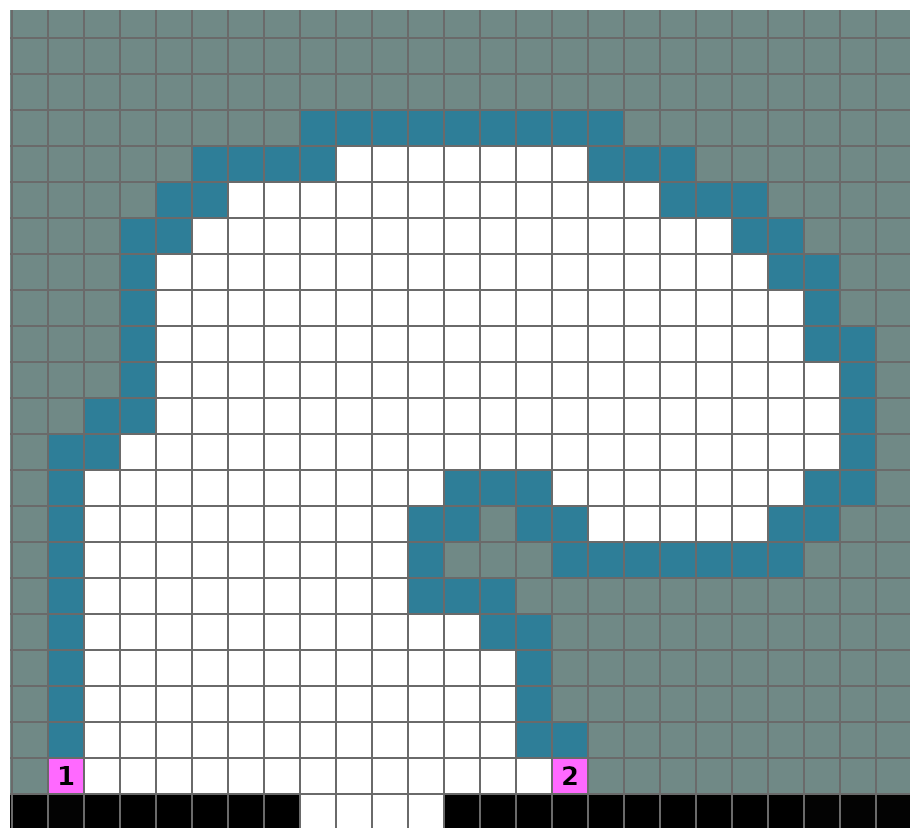
\includegraphics[clip=true, width=0.40\textwidth]{imagenes/ejemploSimpCub/a2.png}}
  \subfloat[Se elige un nuevo $\mli{fs}$ y se actualizan $\mli{UF}$, $\mli{FS_i}$ y $\mli{FP}$.]{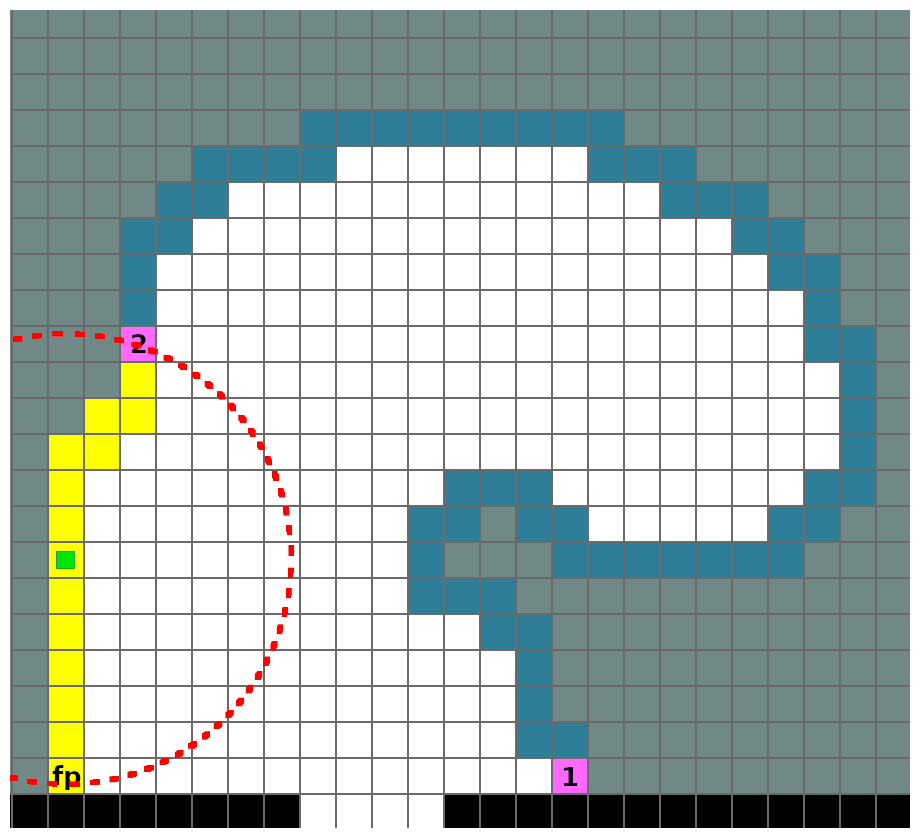
\includegraphics[clip=true, width=0.40\textwidth]{imagenes/ejemploSimpCub/b5.png}}
  \subfloat[Se elige un nuevo $\mli{fs}$ y se actualizan $\mli{UF}$, $\mli{FS_i}$ y $\mli{FP}$.]{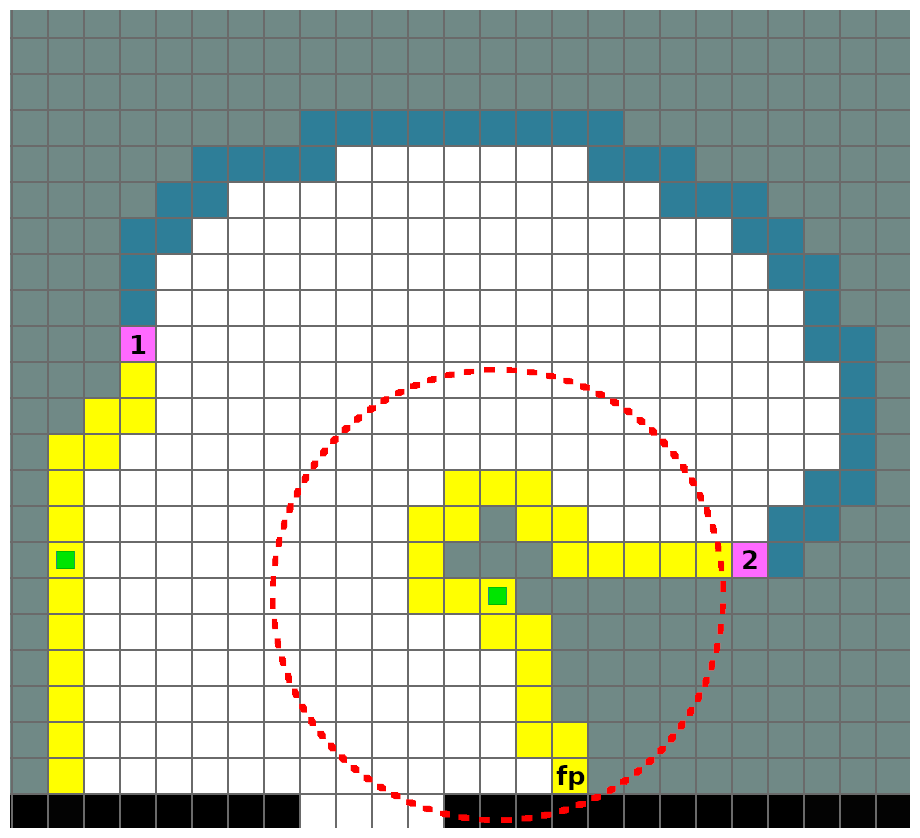
\includegraphics[clip=true, width=0.40\textwidth]{imagenes/ejemploSimpCub/c5.png}}

  \subfloat[Se elige un nuevo $\mli{fs}$ y se actualizan $\mli{UF}$, $\mli{FS_i}$ y $\mli{FP}$.]{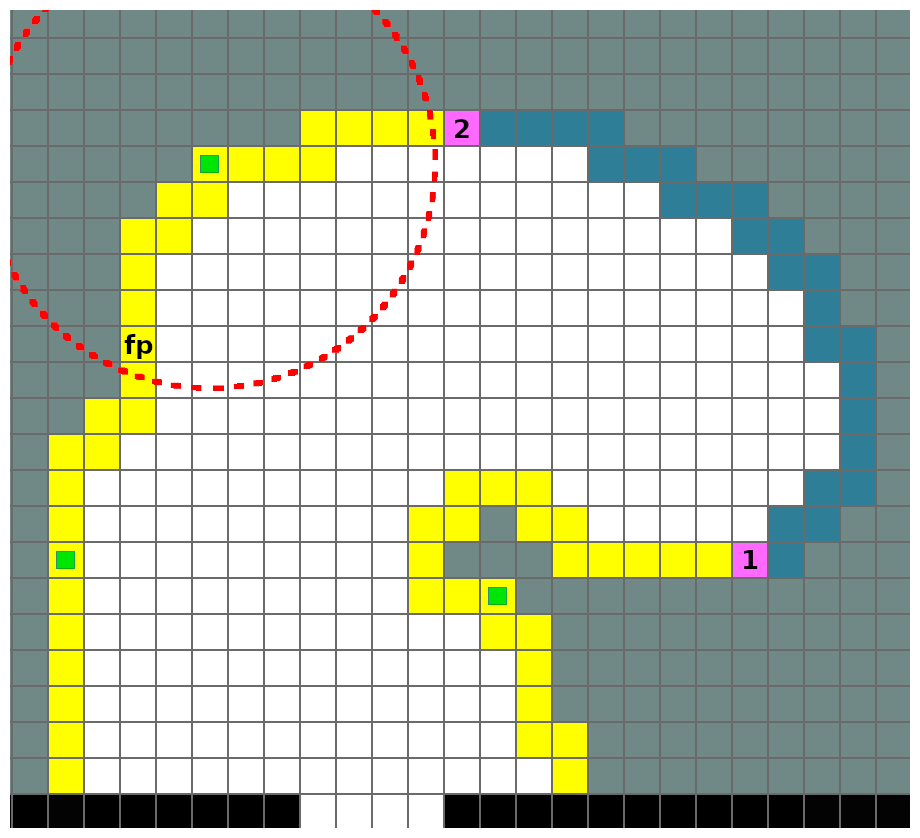
\includegraphics[clip=true, width=0.40\textwidth]{imagenes/ejemploSimpCub/d5.png}}
  \subfloat[Se elige un nuevo $\mli{fs}$ y se actualizan $\mli{UF}$, $\mli{FS_i}$ y $\mli{FP}$.]{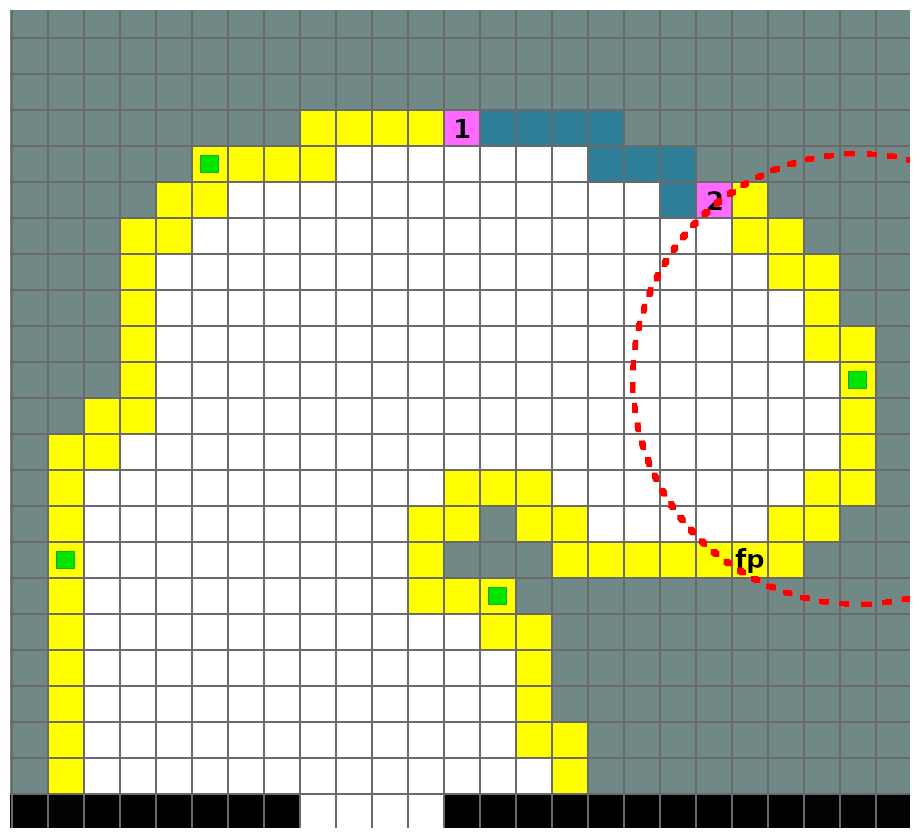
\includegraphics[clip=true, width=0.40\textwidth]{imagenes/ejemploSimpCub/e5.png}}
  \subfloat[Se elige un nuevo $\mli{fs}$ y se actualizan $\mli{UF}$, $\mli{FS_i}$ y $\mli{FP}$.]{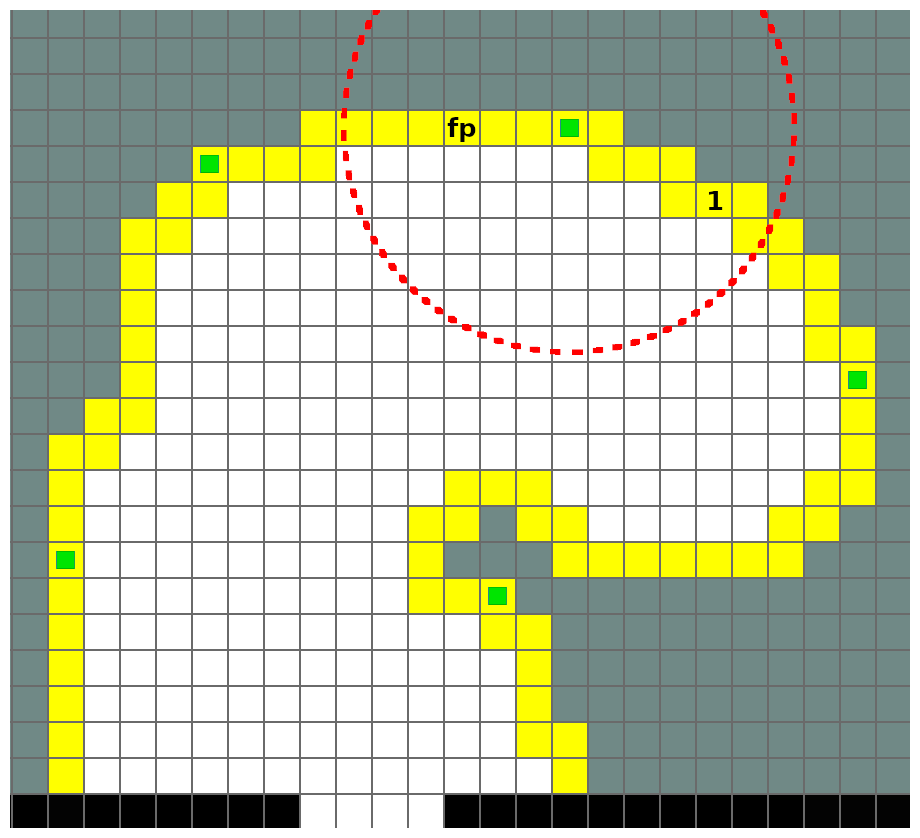
\includegraphics[clip=true, width=0.40\textwidth]{imagenes/ejemploSimpCub/f4.png}}

  \subfloat[$\mli{UF}=\emptyset$ por lo que el algorimo finaliza.]{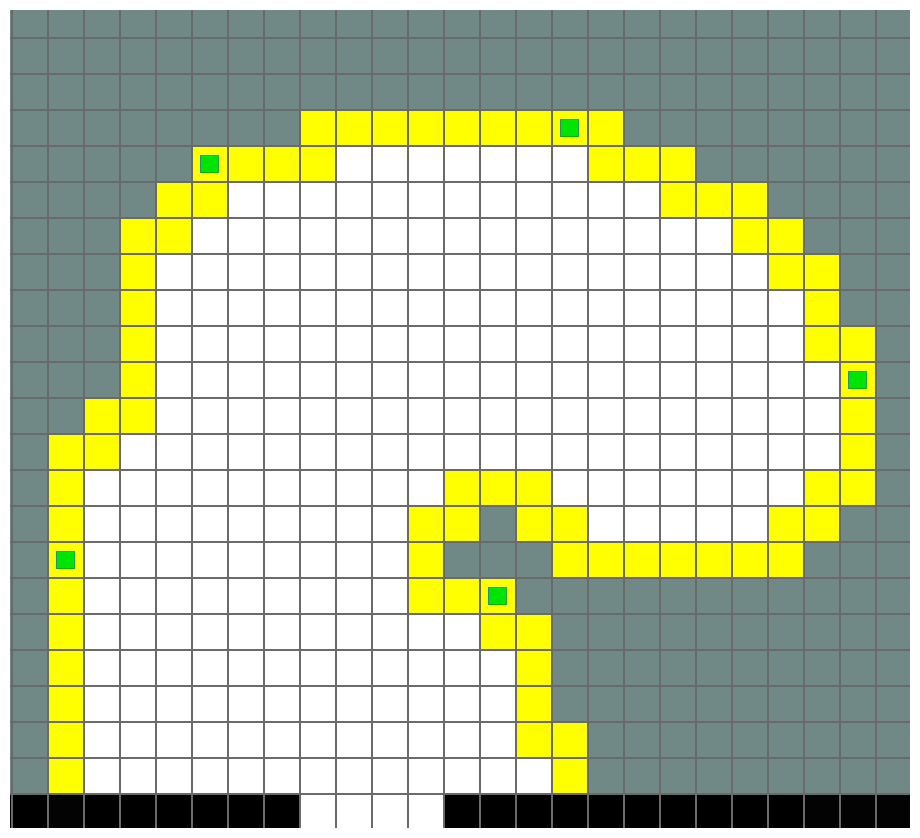
\includegraphics[clip=true, width=0.40\textwidth]{imagenes/ejemploSimpCub/zfinal1.png}}
  \subfloat[Resultado final.]{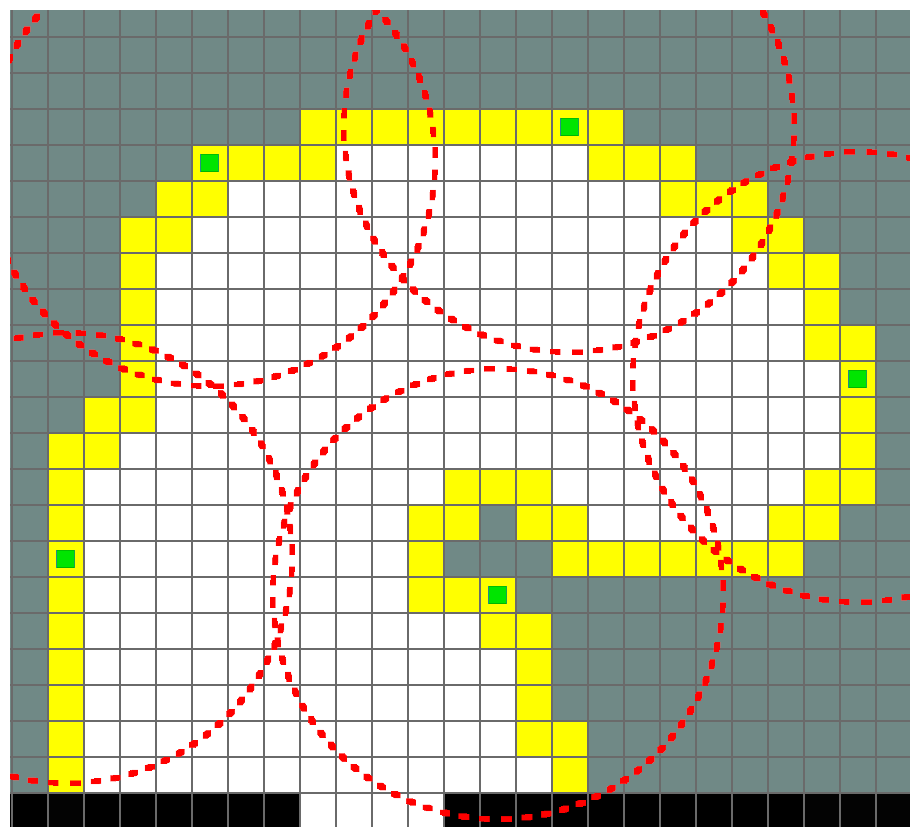
\includegraphics[clip=true, width=0.40\textwidth]{imagenes/ejemploSimpCub/zfinal2.png}}
  % \subfloat[$\mli{UF}=\emptyset$ por lo que el algorimo finaliza.]{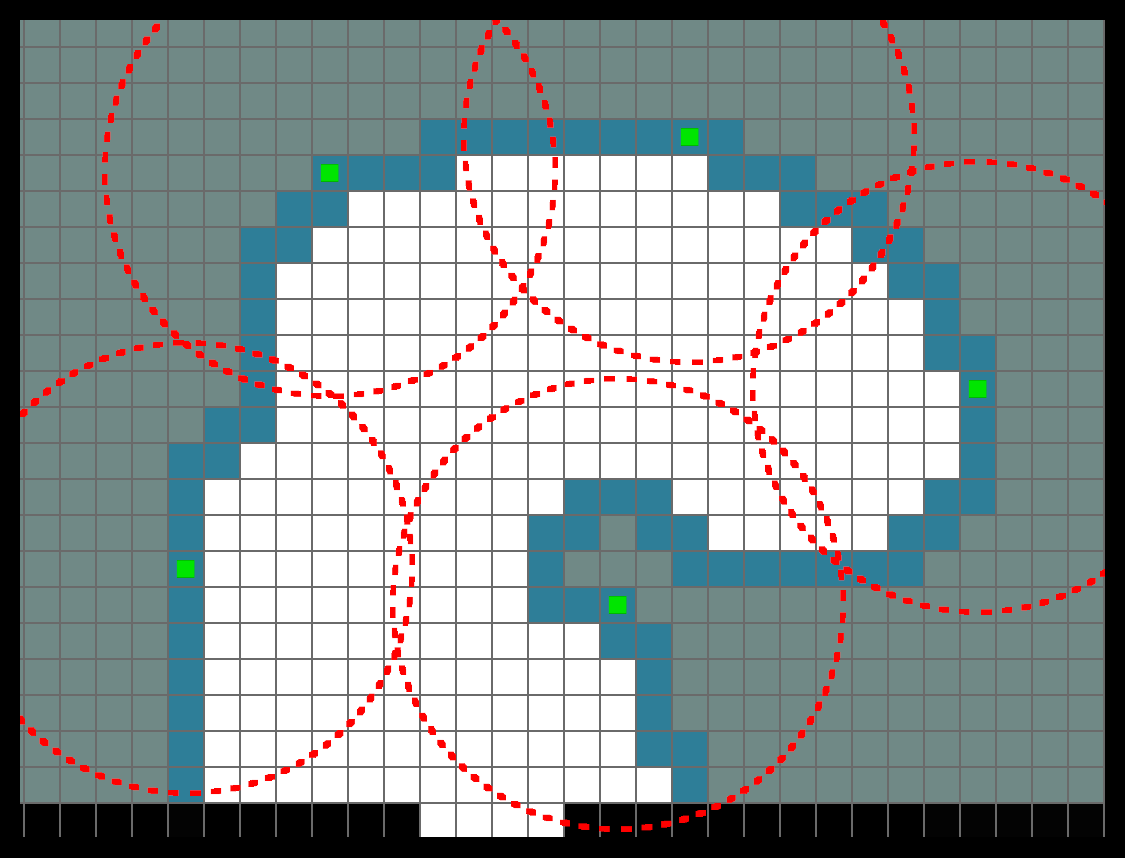
\includegraphics[clip=true, width=0.40\textwidth]{imagenes/ejemploSimpCub/zfinal3.png}}

  \caption[Proceso de simplificacion de fronteras según cubrimiento.]{Proceso
    de simplificacion de fronteras según cubrimiento.  Las fronteras de
    $F_i$ se indican con azul si pertenecen a $\mli{UF}$ y con amarillo de lo
    contrario. Con magenta se indican las celdas en $\mli{FP}$ siendo la
  numeracion su orden en la cola y $\mli{fp}$ la ultima desencolada. Las fronteras significativas se indican con
verde, siendo las circunferencias rojas de radio $rango=5.6$ (largos de celda) centradas en estas indicadores de su cubrimiento.}\label{fig:ejemploFSCub}

\end{figure}


\section{Asignación de tareas}
% Comentar el tema de que uso wurm, que cambio como obtengo el gvd haciendo uso de una variante del metodo inc presentado en Lau que tenia esas mejoras que se mencionaron en \ref{subsec:constGVDInc}. Decir que se va a comentar a detalle las variaciones desarrolladas la seccion \ref{sec:MiConstGVD}. 

Cuando un robot se encuentra ocioso este le solicita a la central que le asigne
una nueva tarea, esto desencadena un proceso de asignacion de
tareas que se describe a lo largo de esta seccion.

La asignación de objetivos se basa en la idea presentada en
\ref{subsec:wurmCoord}, que sostiene que es conveniente que los robots se
asignen a los objetivos de forma que estos se distribuyan uniformemente sobre
las habitaciones y corredores de un entorno estructurado, que se corresponden
las regiones (tambien llamados segmentos) de un mapa topológico (seccion
\ref{subsec:mapas}).

La asignación de objetivos consiste una subasta donde los objetivos de
exploracion son subastados entre los robots. La subasta se puede separar en
tres partes, \emph{obtencion de informacion}, \emph{valuacion} y
\emph{resolucion}. La \emph{obtencion de informacion}, es la etapa en la cual
todos los datos necesarios para llevar adelante la subasta (los objetivos de
exploracion) son determinados. La \emph{valuacion} abarca la distribuicion de
la informacion obtenida desde la central hacia los robots, el juicio de valor
de cada robot a cada objetivo recibido y el posterior envio de estas
valoraciones desde los robots hacia la central. La \emph{resolucion} contempla
la recepcion de las valoraciones por la central, un postprocesamiento sobre
estos, la asignacion de objetivos a robots segun la valoraciones y los
segmentos a los cuales pertenece cada objetivo, finalizando con la notificacion
del objetivo que le fue asignado a cada robot.

Con respecto a la separacion del problema de asignación de tareas mencionada en
la seccion \ref{sec:exploracion}, que establece dos partes, la identificacion
de objetivos y la asignación de objetivos; la primera forma parte de la
\emph{obtencion de informacion}, y la segunda se corresponde con el el resto de
lo que se describe en esta seccion.

% Para que la subasta sea llevada a cabo se deben distribuir los objetivos de
% exploracion entre los robots para que estos asignen valores a cada uno segun
% que tan conveniente les es llegar a ellos. Posteriormente los robots deben
% enviar las valuaciones realizadas a la central,

% la cual debera resolver que
% objetivo le corresponde a que robot segun las valuaciones recibidas y los
% segmentos en dode se ubican los objetivos, procurando distribuir lo mas posible
% a los robots sobre los segmentos. %, el metodo utlizado para lograr este se
% describe en \ref{subsec:MiResSub}. Finalmente la central notifica a cada robot
% su objetivo asignado.

% En resumen la subasta consiste en valuacion y resolucion. 
% valuacion: mandar los objetivos y esperar por sus valuiaciones.
% resolucion: resolucion y informar a laos robots

% asignación de objetivos se puede resumir en:
% \begin{enumerate}
%   \item Identificación de objtivos
% \end{enumerate}

% Para esto, una vez identificados los objetivos segun lo que se presenta en la
% sección \ref{subsec:MiSimp}, cada objetivo se le asigna la region que le
% corresponde en el mapa topológico contruido (seccion \ref{subsec:MiMapTOp}(

% \subsection{Mapa topológico}\label{subsec:MiMapTOp}


% \subsection{Protocolo de susbasta}\label{subsec:MiProtSub}
% Como se comentó anteriormente, la estación central es la encargada de la subasta de segmentos. Los robots son quienes recopilan la información, arman su mapa local y lo envían a la central, que por medio del modulo combinador de mapas, crea un mapa global. Este mapa global es convertido en una grilla de ocupación y segmentado a partr de un GVD. 
% Adicionalmente, fue reutilizada la implementación del algoritmo K-means para obtener las fronteras más significativas según el radio del robot, como fue explicado en al sección 2.1.

% Comentar proceso, enfasis en como es que funciona el flujo: pedido de los robots, identificacion, robots a valuar, recibir valuaciones, asignar y mandar asigaciones a los robots.

% Deternerse en cada parte explicando detalles.

% El pedido no es muy complejo.

% ID ya se explico.

% Envio es directo, la valuacion tiene algunos detalles.

% \subsubsection{Recepcion de valuaciones}
% Recepcion, aca esta el protocolo de recepcion, quizas es pertinente comentarlo por lo menos por arriba.
% \subsubsection{Envio de asignaciones}
% Mandar asignaciones es casi que trivial

\subsection{Obtencion de informacion}
Como se menciono todo comienza cuando un robot ocioso solicita un tarea a la
central, esto desencadana una nueva subasta de no encontrarse una en curso. Si
existe una en curso el robot recibira una tarea cuando esta termine, no es
necesario iniciar otra.

La etapa de \emph{obtencion informacion} es la primera etapa en llevase a cabo
al iniciarse la subasta. La informacion que se obtiene en esta son los
objetivos de exploracion, un GVD y las regiones del mapa mapa topológico del
entorno explorado que con el motivo de identificar en que segmento se encuentra
cada objetivo de exploracion, para porsteriomente poder asignar distribuyendo a
los robots sobre estos. 

La identificacion de objetivos se lleva a cabo con el metodo descrito en la
sección \ref{subsec:MiSimp}.

El mapa topológico se construye con la tecnica descrita en la seccion
\ref{subsec:mapaTopGVD} que se basa en el uso de un GVD. Uno de los cambios
principales con respecto al trabajo original de \cite{wurm2008coordinated} es
la forma en la cual se contruye el GVD. En el trabajo original se hace uso de
un metodo de construccion no incremental, en este proyecto con el motivo de
alcanzar una implementación que logre funcionar en tiempo real (seccion
\ref{subsec:constGVDInc}) se reemplaza por una variante del algoritmo
incremental \emph{brushfire dinamico} que se presentará en la seccion
\ref{sec:MiConstGVD}.


\subsection{Valuacion} \label{subsec:MiValSub}

Luego de obtenida la informacion se da comienzo a la estapa de \emph{valuacion}
distribuyendo dicha informacion desde la central hacia los robots. Cuando un
robot recibe la informacion este asigna dos valores a cada objetivo, el largo
del camino hacia a el y un costo asociado a la complejidad del camino.

Calcular el largo de un camino implica determnar el camino en sí. El camino se
calcula de forma distinta dependiendo de la clase de objetivo, existen dos,
triviales y no triviales.

Los objetivos triviales se definen como los objetivos para los cuales el
segmento de recta que existe entre el robot y el objetivo no contiene
obstaculos, de lo contrario el objetivo es no trivial. Para determniar esto, se
discretiza el segmento de recta en celdas \cite{foleyphillips} y se comprueba
en el mapa global (grilla de ocupacion) almacenado en el robot, alguna de las
celdas tiene un estado ocupado.

El camino en objetivos triviales se determina como dicho segmento de recta que
existe entre el robot y el objetivo, que se encuentra libre de obstaculos. 

En el caso de los objetivos no triviales se hace uso del GVD recibido como
parte de la informacion de la subasta, aprovechando que este constituye un
\emph{roadmap} (seccion \ref{subsec:mapacarr}). El GVD viene representado
como el conjunto de celdas que abarca, el proceso para construir el camino puede dividir 
en tres partes cada una asociada a una de las propiedades que caracterizan a un
\emph{roadmap}: accesibilidad, conectividad y capacidad de salida. La parte asociada
accesibilidad consiste en encontrar un camino desde el robot al GVD, lo cual se
hace a traves de un \emph{breadth-first search} (BFS), se comienza en la celda
asociada a la posicion del robot y se detiene apenas se visita una celda $c_1$
perteneciente al GVD. La que se relaciona con la capacidad de salida es analoga a la
accesibilidad pero el camino va desde el objetivo a alguna celda $c_2$ del GVD.
Por ultimo la parte vinculada con la conectividad se basa en establecer un
camino sobre las celdas del GVD desde $c_1$ a $c_2$, lo cual se hace aplicando
algoritmo $A^*$. Conectando esos tres caminos se obtiene el camnino completo.

El costo asociado a la complejidad en el caso de objetivos triviales se
determina como el tiempo estimado que demora el robot en rotar de forma que su
parte delantera apunte hacia el objetivo. Y en el caso de objetivos no
triviales se utiliza la maxima penalizacion usada para objetivos no triviales.
El proposito de esto es diferenciar los objetivos triviales sin beneficiar a
los objetivos no triviales. Este costo se aplica para incentivar a que el robot
ontinue siendo asignado a los objetivos triviales que tiene por adelante al
explorar.

Obtenidos ambos valores para cada objetivo estos se envian hacia la central
junto a la ubicacion actual del robot, siendo toda esta informacion en su
conjnto considerada una valuacion. \todo{o mensaje de valuacion, como quede mejor}

% De esta
% forma los objetivos triviales se valuan distinto segun que tanto tiene que
% rotar el robot para llegar a ellos y los objetivos no triviales tendran un
% costo no mayor al del peor objetivo no trivial.

% como el conjunto de celdas que abarca, el proceso para construir el camino es
% se puede dividir en encontrar tres subcaminos cada uno relacionado a una de las
% tres propiedades de un roadmap: accesibilidad, conectividad y capacidad de
% salida. La accesibilidad consiste en encontrar un camino desde el robot al GVD,

% La valuacion abarca la distribuicion de los objetivos de exploracion desde la
% central hacia los robots, la asignación de valores que cada robot debe hacer a
% cada objetivo y el posterior envio de estas valoraciones desde los robots hacia
% la central. 

\subsection{Resolución} \label{subsec:MiResSub}
% La resolucion es el proceso de asignar los objetivos La resolucion contempla
% la recepcion de las valoraciones por la central, la asignacion de objetivos a

% robots segun y la notificacion del objtivo asignado a los robots. 
% de exploracion a los
% robots. 
\subsubsection{Recepcion de valuaciones}
La resolucion comienza con la recepcion de las valuaciones realizadas por
los robots. Al recibirse la primera valuacion existe una ventana de tiempo en
la que la central continuara recibiendo nuevas valuaciones. Terminada esta
ventana se ejecuta un algormitmo que resulta en la asignacion de objetivos a
los robots.

El proposito de la ventana es que en escenarios reales los robots pueden dejar
de comunicarse por alguna razón (desconexiones de red, accidentes que dejen a
los robots sin funcionar, entre otros), por lo tanto esperar por las
valuaciones de todos los robots puede ser una espera infinita.

Dado que el problema que los robots deben resolver para generar las valoraciones es
similar, se asume que el tiempo se demora en generar las valoraciones tambien
es similar, adicionalemtente dicho tiempo es proporcional al area del
mapa que se encuentra explorada, por lo tanto se opto por utilizar una ventana
dinámica de un tamaño que, considerando lo que demoraron las valoraciones de
los robots en la subasta anterior, sea lo suficientemente grande como para que
todos los robots que esten en condiciones de responder con sus valoraciones
tengan el tiempo necesario para hacerlo.

Notar que una vez que se reciben las valoraciones de todos los robots
funcionales es innecesario continuar esperando, por lo tanto de recibirse
dichas valoraciones la ventana de resolución es terminada prematuramente
evitando esperas innecesarias.

Siendo $tr_i$ el tiempo que paso desde la recepcion de la primera valuacion
hasta el comienzo de la ejecucion del algormitmo de asignacion y $vr_i$ la
duracion de la ventana $i$ definida en \ref{eq:ventanaVals}.

\begin{equation} 
  vr_i = 
  \left \{ 
    \begin{aligned}
      0.5s                            \ \ \ \ \ \ \ \ & si\ i = 0\\ 
      max(0.5s + 2tr_{i-1}, vr_{i-1}) \ \ \ \ \ \ \ \ & si\ i > 0
    \end{aligned}
  \right .
  \label{eq:ventanaVals}
\end{equation}

El valor de la duracion $v_i$ resulta de asumir que de una subasta a la
siguiente no se demorara más del doble del tiempo en obtener las valuaciones de
todos los robots, dando un margen de error de 0.5 segundos, especialmente útil
cuando $rt_i$ es muy pequeño. Lo asumido se corresponde con lo ocurre en las
pruebas realizadas.

% por lo que sería contraproducente no esperar por la valoración de
% algún robot ya que dicha espera es mínima en comparación con lo que un robot
% debe esperar en caso de no ser considerado para la resolución.

% Para cumplir con el propósito propuesto se podría decir que la ventana sea de
% un tamaño muy grande o infinita, lo cual en un entorno simulado como el que se
% basa este trabajo no generaría problemas ya que los robots siempre pueden


% y como estas se guardan al recibirse
\subsubsection{Algoritmo de asignacion de objetivos}
% Segun lo explicado en la seccion anterior
Cuando la central recibe una valuacion de un robot $r_i$, esta se encarga de
procesar la informacion contenida en la valuacion de forma de obtener un unico
costo $c_{i,j}$ del robot $r_i$ a cada objetivo $o_j$. Para un objetivo en
$o_j$ la valuacion del robot $r_i$ contiene el costo $\mli{cca}_{i,j}$ del camino de
$r_i$ a $o_j$ y el costo $\mli{cco}_{i,j}$ asociado a la complejidad de dicho camino.
Adicionalmente a traves de la posicion recibida de $r_i$ se determina un descuento 
$\mli{dse}_{i,j}$ que toma un valor constante menor a cero ($-10$ en al
implemetnacion) si el robot $r_i$ pertence al mismo segmento que el objetivo
$o_j$ y cero de lo contrario. Finalmente el costo $c_{i,j}$ se calcula segun la
ecuacion \ref{eq:costoTot}.

\begin{equation} 
  c_{i,j} = \mli{cca}_{i,j} + \mli{cco}_{i,j} + \mli{dse}_{i,j}
  \label{eq:costoTot}
\end{equation}

Los costos $\mli{cca}_{i,j}$ y $\mli{cco}_{i,j}$ tienen como proposito
penalizar en la asignacion a los objetivos segun la dificicultad asociada a los
caminos que llevan a esto. Por otro lado el descuento $\mli{dse}_{i,j}$
incentiva que los robots se mantengan explorando un mismo segmento, lo cual
desencadena comportamientos deseables como el de que un robot continue
explorando un mismo corredor, revelando rapidamente la estructura de un entorno
estrucutrado.

% Los robots envian a la central dos valores junto a su posicion, cuando la central lo recibe estos se 

% esto, la posicion de dicho robot y
% dos valores, al recibirse la valuacion en la central dichos valores son
% procesados de forma

% La version original de \cite{wurm2008coordinated} lleva a cabo la asignacion
% utilizando el metodo hungaro. Este  
% de forma optima en $O(n^3)$ siendo $n$ el numero de tareas.

Con estos costos costos como insumos se ejecuta un algorimo de asignacion de
objetivos a robots, este tiene como proposito asignar objetivos a los robots de
que estos se distribuyan sobre los segmentos (seccion \ref{subsec:wurmCoord}).
\todo[inline]{El metodo hungaro capaz no considera que el numero de robots
  asigandos a un segmento debe ser menor que el numero de fronteras que tiene
  ya que no tiene sentido asignar a un robot a un segmento si este no tiene
  objetivos disponibles. Habria que ver bien como funciona el metodo hungaro,
  pero creo que es una asignacion robot-segmento que no considera otra cosa que
  el costo, num robots y num segmentos, por lo tanto el num de fronteras de un
  segmento no se estaria considerando.}

% El algorimo \ref{alg:resolucionsubastasegmentos} presenta un pseudocodigo del
% algormitmo de asigacion donde $R$ el conjunto de los identificadores de los
% robots, $O$ el conjnto de los identificadores de los objetivos y $Costos$ el
% conjunto los $c_{i,j}$ computados a partir de las valuaciones recibidas
El algorimo de asigacion, se corresponde al algorimo
\ref{alg:resolucionsubastasegmentos}, donde $R$ es el conjunto de los
identificadores de los robots de los cuales se recibieron valuaciones, $O$ el
conjnto de los identificadores de los objetivos valuados, $Costos$ un conjunto
de tuplas $(c_{i,j},r_i,o_j)$ los $c_{i,j}$ computados a partir de las
valuacion recibida de $r_i$ para $o_j$ y $S$ el conjunto de
segmentos. La funcion $segmento : O \rightarrow S$ dado un objetivo devulve el
segmento al que pertence y la funcion $\#objetivos : S \rightarrow N$ devuelve
el numero de objetivos en un segmento.
% Los conjuntos $O_1$,$O_2$,...,$O_k$,...,$O_{|S|}$ contienen los
% objetivos que estan dentro de un segmento $s_k\in S$.

\vspace{1cm}
  
\begin{algorithm}[H]
\SetAlgoLined
  \SetKwInOut{Input}{Entrada}
  \Input{$R, O, S, Costos$} % O_1, O_2,...,O_{|S|}$}
%   // PARTE 1
    $segObjs :=$ Multiconjunto vacio 

  
%   /// recorrida de todos los elementos del diccionario, con el propósito de construir segFrontColaPrio
    \ForEach{$s_k \in S $}{ 
     %ALT1 segObjs.encolar($|O_k|$)\\
     %ALT2 $segObj = segObj \cup \{|O_k|\}$\\
     $segObj = segObj \cup \{\#objetivos(s_k)\}$\\
    }
    
    $numSegs := |S|$\\
    $numRobs := |R|$\\
    $converge := false$\\

    \While{$\lnot (segObjs = \emptyset \lor converge$)}{
      $cocienteDist := numRobs\ \ div\ \ numSegs$\\
      $restoDist    := numRobs\ \ mod\ \ numSegs$\\
    
      $segObj := min\ segObjs$\\
      $segObjs := segObjs - segObj$\\
    
      $converge := (segObj > cocienteDist) \lor (restoDist = 0 \land segObj = cocienteDist)$\\
      \If{$\lnot converge$}{
        $numRobots := numRobots - segObj$\\
        $numSeg := numSeg - 1$\\
      }
    }
%   // PARTE 2
    $asignaciones := \emptyset$\\

    $segRobNums :=$ diccionario de $S$ a enteros, siendo 0 el entero asignado por defecto\\   

    \While{$R \neq \emptyset \land O \neq \emptyset$}{
      $(c_{i,j}, r_i, o_j) := min\ Costos$ \tcp{Tupla de $Costos$ con minimo $c_{i,j}$}
      $Costos := Costos - (c_{i,j}, r_i, o_j)$\\
      $s_k := segmento(o_j)$\\
      $distribuido := segRobNums[s_k] < cocienteDist \lor (restoDist > 0 \land segRobNums[s_k] < cocienteDist + 1)$\\
      \If{ $r_i \in R \land o_j \in O \land distribuido$ }{
        $asignaciones := asignaciones \cup (r_i,o_j)$\\
        $segRobNums[s_k] := segRobNums[s_k] + 1$\\
        $R := R - r_i$\\
        $O := O - o_j$\\
        \If{$segRobNums = cocienteDist + 1$}{
           $restoDist := restoDist - 1$\\
        }
      }
    }
  \Return asgnaciones 
    
 \caption{Asigacion de robots a objetivos}
 \label{alg:resolucionsubastasegmentos}
\end{algorithm}

El algorimo se puede dividir en dos partes, el \emph{calculo de valores}
$cocienteDist$, $restoDist$ (lineas 1-18) y la \emph{asignacion distribuida} (lineas
19-36). 

Los valores $cocienteDist$ y $restoDist$ se utlizan para lograr una asignacion
distribuida sobre los segmentos conisderando los objetivos contenidos en cada
uno. La distribucion deseada se corresponde con la distribucion que se logra al
hacer $N$ rondas en las que se asigna un solo robot por segmento con tenga
objetivos sin asignar. La ronda $N$ termina cuando no quedan robots o objetivos
por asignar. Si existen menos objetivos que robots se tiene que la ronda $N$
culmina con todos los objetivos asignados y algunos robots ociosos. De existir
mas objetivos que robots luego de la ronda $N$ se pueden tener segmentos cuyos
objetivos estan todos asignados y se tienen segmentos dentro de los que 
existen objetivos sin asignar, la distribucion sera unfirme sobre estos ultimos
segmentos. Es decir los $K$ segmentos que tienen objetivos sin asignar
cumpliran con (\ref{ec:uniform}), existiendo $restoDist$ segmentos con
$N=cocienteDist+1$ robots asignados y $K-restoDist$ segmentos con
$cocienteDist$ robots asignados. El \emph{calculo de valores} se lleva a cabo
inicializando $cocienteDist$ y $restoDist$ asumiendo una distribucion
completamente uniforme (lineas 5-6 y 9-10 primera iteracion), sin considerar si
es posible dado el numero de objetivos en cada segmento. Luego de forma
iterativa, segmento a segmento y comenzando por los que tienen menos objetivos
(lineas 11-12), comprobar si son de los segmentos cuyos objetivos seran todos
asignados (linea 13) y de serlo ajustar los valores para que la distribucion
sea uniforme en el resto de conjuntos (lineas 14-17 y 9-10). Las iteraciones
continuan hasta que solo quedan los segmentos en los que quedaran objetivos sin
asignar (linea 8), cuando esto sucede se dice que $cocienteDist$ y $restoDist$
convergen.
% a los valores consistentes con la distribucion deseada.

Con los valores $cocienteDist$ y $restoDist$ calculados la \emph{asignacion
distribuida} consiste en retirar las tuplas $(c_{i,j},r_i,o_j)$ de $Costos$
comenzando por las de menor costo $c_{i,j}$ (lineas 22-23) y para cada una de
estas asignar $r_i$ a $o_j$ (lineas 27-33), si $r_i$ y $o_j$ no forman parte de
ninguna de las asiganciones realizadas hasta el momento, y si la asignacion
mantiene la distribuicion deseada (lineas 25-26). Esto se repite hasta que
todos los robots estan asignados o que no quedan mas objetivos por asignar
(linea 21).

% , estos se calculan de forma que todos los segmentos tengan todos sus objetivos asignados a robots, un numero de robots asignadosk

En resumen, la central asigna a los robots a objetivos considerando los costos
de forma voraz y con la restriccion de distribuir los robots sobre los
segmentos considerando la cantidad de objetivos que contienen. Luego de
ejecutar el algorimo de asigacion la central informa a cada robot el objetivo
que le fue asignado, quedando a la espera de nuevos pedidos por parte de los
robots para comenzar una nueva subasta. 


\section{Grafo generalizado de Voronoi}\label{sec:MiConstGVD}

Considerando los problemas de eficiencia del algorimo \emph{brushfire} (seccion
\ref{subsec:constGVD}) y los problemas de su version incremental
\emph{brushfire dinamico} (seccion \ref{subsec:constGVDInc}) como fue propuesta
originalmente en \cite{kalra2009incremental}, se decidio basar la construccion
del GVD en la version de \emph{brushfire dinamico} propuesta en \cite{Lau2013},
a la que se estara haciendo refencia cuando se mencione \say{\emph{brushfire dinamico}
original} desde este punto.

A lo largo de esta seccion se explicaran las conicidencia y cambios entre
\emph{brushfire dinamico} y la variante de este implementada en este proyecto.

\subsection{Pertenecia}
La implemetacion realizada en proyecto mantiene las olas conistentes e
inconsistentes para el calulo incremental de mapas de distancia. Tambien
mantiene la idea que las olas inconsistentes remueven las celdas que atraviesan
del GVD y la idea de que las celdas en las cuales las ondas consistentes se
detienen son las celdas cuya pertenencia al GVD se comprueba.

\todo{seguir desde aca}
El cambio que se hace es en el criterio con el cual se comprueba la pertenencia
de una celda. En el \emph{brushfire dinamico} original se hace EXPLICAR
CON LO DE MAS ABAJO. En esta implementacion cambia, al existir un choque de
olas primero se establecen los pseudosources y luego de existir dos
pseudosources no adjacentes entre si la celda pertenece.

Explicar definicion de un pseudosource, y porque esto termina siendo distinto
que lo que se plantea en el \emph{brushfire dinamico} original.

Oportunidad de comentar que mejora sobre lau porque perminte generar gvd en
lugares a dist 1 de los obstaculos, cosa que lau no permite ni explica porque.

Explicar que quizas se relacione al tema corredor de largo 2 que se va a explicar en \ref{subsec:filt}.

\subsection{Filtrado}\label{subsec:filt}
Los vetices que en una iteracion se determina que deben pertenecer al GVD segun
el criterio de pertenecia aplicado en las celdas en las cuales se detiene una
ola consistente, pasan por un filtrado extra. Este filtrado busca evitar lineas
discretizadas de dos celdas de grosor que violan la propiedad \say{sparceness}
GVD.

As discussed before, different paths on the Voronoi graph correspond to
topologically different routes in the environment (sparceness property). To preserve this property
for GVDs on grid maps, thin Voronoi lines, i.e., being one pixel wide, are
desired.

% Spacrceness:Their application as roadmaps is an appealing technique for path
% planning, since they are “sparse” in the sense that different paths on the
% graph correspond to topologically different routes with respect to obstacles.
% This

En el \emph{brushfire dinamico} original el filtrado se lleva a cabo haciendo
uso de patrones con los cuales se comprueba si el GVD queda o no disconexo

Our optional pruning step erodes 2-pixel-wide Voronoi lines. Therefore, all
new Voronoi cells are inserted into a priority queue and processed by the
pruning stage. The image operator patterns shown in Fig. 6 (solo poner
8-connected) match whenever the center cell s provides connectivity for one or
more of its adjacent cells. In any pattern, a $1$ matches voro(s) = true, while
$0$ stands for voro(s) = false, and empty fields are ignored. Where indicated
by arrows, the same pattern is applied in all unique 90 degree rotations

The second phase implements the actual pruning step. In increasing order of
distance, the enqueued cells are iteratively popped from the priority queue. If
such a cell has more than one neighbor on the GVD and is not required to keep
the GVD connected, it can be removed from the GVD without affecting its
topology. Again, this is tested using the image operator patterns: if none of
the connectivity patterns match at the cell location, the cell is not required
in the GVD.

Enfasis en $P^8_1$ que indica que las celdas con un solo vecino deben pertenecer al GVD.

En el caso de la implementacion del proyecto se comprueba si el GVD queda
disconexo aplicando la tecnica presente en \cite{zhang1984fast},
adicionalemtente evitando filtrar celdas con una sola celda adyacente en el GVD
y con 2 celdas ayacentes en el GVD si estas se detectan en un corredor.

Explicar caso corredor. comentar que no se considera en lau, quizas se arregla no permitiendo dist = 1

% \subsection{Limpieza de aristas}
% La limpieza de aristas es una tecnica aplicada solo en la implementación del
% proyecto esta permite generar GVD mas limpios. 

\subsection{Consideraciones de segmentacion}

% segun si las celdas ocupadas mas cercanas $oc_1$ y $oc_2$ de

Dado que se segmenta el entorno segun el metodo que se comenta en la seccion
\ref{subsec:mapaTopGVD}, es necesario encontrar los puntos criticos y lineas
criticas asociadas al GVD construido segun las cuales se dividen los segmentos.
Recordando que el GVD contruido esta discretizado en celdas y que los conceptos
de puntos y lineas criticas se definen en espacios continuos es necesario
adaptarlos. 

En el caso de los puntos criticos, dadas celdas $\mli{GVDD}$ que conforman al
$GVD$ discretizado y considerando el mapa de distancia subproducto de
\emph{brushfire dinamico} como la funcion de despeje discretizada $DD : C
\rightarrow R$, se puede definir el conjunto de las celdas criticas (puntos
criticos discretizados) $\mli{CrD}$ segun (\ref{eq:critDisc}). 

\begin{equation}
  % p\ \in C \iff p \in \mli{GVD}\ \land \ D(p) < D(p')\ \forall p' \in Ady(p) 
  \mli{CrD} = \{c\ \in C_{\mli{GVD}} : \exists c_g \in ady(c), D(c_g) > D(c), \forall c_l \in ady(c), D(c) \leq D(c_l) \} \label{eq:critDisc}
\end{equation}

Explicar que esto no es exactamente un minimo local, si no que extienede la
nocion a casos como los de las figuras que saque, en donde de ser solo minimo
local no hay criticos pero al decir que no hay menors y hay al menos uno mayor
si, cosa que es deseable dado que efectivamente los ejemplos mostrados son
puertas y este tipo de situacion es usual en puertas sobre las esqunas de las
habitaciones.

Explicar (implica redefinir $\mli{CrD}$ , creo que lo mejor es plantear
condiciones a cumplir siendo la de \ref{eq:critDisc} una) los criterios filtros
utilizados para los puntos criticos.

Para adaptar el concepto de las lineas criticas es necesario adaptar primero el
concepto de puntos base de un punto en el GVD, que son los puntos mas cercanos
de los generadores que generan su pertenencia al GVD. En \emph{brushfire
dinamico} no se manejan los generadores base de forma directa, la pertenencia de
una celda al GVD se determina en cada choque de celdas. Dado un choque de
celdas que involucra a las celdas $c_1$ y $c_2$, sean $oc_1$ y $oc_2$
respectivamente sus celdas ocupadas más cercanas se considera que si $oc_1$ y $oc_2$
son adyacentes entonces pertenecen al mismo generador generalizado y de lo
contrario que pertenecen a distintos generadores generalizados. De esto se
deriva que si $oc_1$ y $oc_2$ no son adyacentes entoces $c_1$ y $c_2$ deben
pertenecer al GVD. De esta forma se logra aproximar el GVD resultante de
considerar generadores conexos y convexos \ref{subsec:GVD}. Dado esto se
definen los puntos que base discretizados $\mli{BPD}_c$ como las celdas
obstaculizadas no adyacentes que generan la pertenecia de una celda $c$ al GVD.
Las lineas criticas discretizadas se definen como las lineas discretizadas
\cite{foleyphillips} definidas entre los centros de las celdas criticas y cada
uno de sus puntos base discritizados.

Establecido esto, es pertinente notar que la implementacion de \emph{brushfire
dinamico} hecha en este proyecto difiere en la original en que esta almacena
las celdas ocupadas que generan la pertenecia de un punto al GVD para ser
utlizados posteriormente como puntos base.

% Tambien se filtran las lineas criticas, como las ideas es que estas se ubiquen en umbrales 

% Desribir problemas de desconexion presentados en las diversas implementaciones? 
% \begin{itemize}
%   \item mencionar los de kalra?
%   \item los generados por considerar dist 1 en lau?
%   \item y mostrar que liu ming aunque no explique que hace bien tambien los tiene?
% \end{itemize}

% Aunque existe una etapa de erosion posterior como en Lau para asegurar la
% sparceness. Comentar que se basa en el A de zhang, que en principio es mas
% eficiente que chequear patrones

% Se mantienen todos los obts a minima distancia, y los que \say{casi} estan a
% minima distancia, siendo estos los puntos bases (puntos mas cercanos a
% generadosres base) tomados en cuenta, segun estos se define si un punto pertenece o no al GVD.

\subsection{Consideraciones sobre el espacio desconocido}
% , la alternativa de que los bordes no sean
% Obstaculos (como esta no aplica a entornos abiertos y genera mas costos) y
Explicar el problema de considerar lo desconocido, como no hacerlo lleva a GVD
disconexos, explicar lo que se encuentra en el estado del arte (explicar como
esta aplica para entornos abiertos) y la alternativa de que las fronteras
(invertidas) sean emisoras de ondas consistentes e inconsistentes y lo
desconocido no sea atravezable por las ondas y porque esto implica mucho menos
costos para mapas cuando estos se comienzan a explorar y se componen de muchas
celdas desconocidas.

Comentar que las celdas con lo desconocido como punto base no genera lineas ni
puntos criticos.

\todo{FEDE: Kalra se ve que el mapa para entorno abierto es consistente con esta tecnica, en el codigo de lau tambien. Pero no se hace referancia a esto}

% \subsection{Segmentacion}
% yo diria de 

% Creo que aca en realidad no habria que comentar mucho si es que hay que comentar, son las mismasideas que las comentadas en \ref{subsec:mapaTopGVD}.

% Quizas mencionar que se usa la descomposicion en componentes conexas y como. 

% Mencionar el uso de sources y pseudosources para hacer lineas criticas. Discretizacion de lineas?

% Algunos resultados?

\section{Planificación}
Describier el proceso a detalle desde que llega un camino, y como este se va
completando poco a poco hasta llegar al objetivo de exploracion al final del
camino.

Tocar por arriba los mecanismos de recuperacion si queda facil.

\subsection{Subobjetivo}
Es un punto intermedio de un camino que lleva a un objetivo, el cual debe ser percibido por los sensores del robot

Un subobjetivo se considera completo si:
\begin{itemize}
  \item Existe una linea recta de grosor minDesiredDistance que lo conectan con
    el robot sin solaparse con ningun obstaculo y tampoco tienen obtaculos a
    minDesiredDistance. 
  \item Esta a meno de una distancia Y (Y puede estar entre
    forcedCompletionTolerance y $\infty$)
\end{itemize}
O si:
\begin{itemize}
  \item Esta a menos de una diatancia forcedCompletionTolerance (mencionada en otra seccion, se puede ver de reorganizar luego)
\end{itemize}

\subsection{Objetivo}
Es el punto final de un camino, debe ser percibidopor los sensores del robot

Un objetivo se considera completo si:
\begin{itemize}
  \item Existe una linea recta de grosor minDesiredDistance que lo conectan con el
    robot sin solaparse con ningun obstaculo y tampoco tienen obtaculos a minDesiredDistance. 
  \item Esta a meno de una distancia Z (Z puede estar entre forcedCompletionTolerance y alcance de sensado)
\end{itemize}

O si:
\begin{itemize}
  \item Esta a menos de una diatancia forcedCompletionTolerance (mencionada en otra seccion, se puede ver de reorganizar luego)
\end{itemize}

\subsection{Objetivos triviales}
Estos objetivos son los que tienen una linea recta de grosor X que lo conectan
con el robot sin solaparse con ningun obstaculo y tampoco tienen obtaculos a
X. X puede ser el maximo tamaño de una puerta o la minDesiredDistance.
\begin{itemize}
  \item Yo use un estimado del max tamaño de la puerta para evitar objetivos
    triviales  que esten en un segmento distinto del que esta el robot
\end{itemize}

Estos objetivos tienen el trato especial de que los camninos planificados a
estos no son sobre el GVD si no que consiten solo en el objetivo trivial.

Esto facilita la navegacion cuando el camino al objetivo es muy facil, es decir es trivial.

\subsection{Objetivos no triviales}

Cuando el objetivo no es trivial lo que se hace es obtener un camnino utilizando el
gvd como roadmap.

Cada punto de este camnio es un subobjetivo menos el ultimo que es el objetivo
en si. El robot siempre se dirige al ultimo subobjetivo/objetivo no competado.

De esta forma notando las condiciones de complecion si Y es grande se tiene 
navegacion libre (delegada a move base, el nivel bajo de la jerarquia) sobre
zonas para las cuales no existen obtaculos mientras que se navega siguientdo el
camnino seguro (provisto por el gvd, nivel alto de la jerarquia) cuando los
objetivos son \say{no deseables} o \say{no seguros}.

Lo que se suele obtener en entornos estructurados es que los robots se mueven
libremente en el interior los segmentos, mientras que para pasar de segmento a
segmento utiliza el gvd para pasar por los pasajes estrechos que consituyen las
puertas.

En el caso de un Y pequeño se tiene una navegacion que sigue de forma mas estricta al GVD.

% Entiendo que Y grande es mejor:
%   `Una prueba para validar esto seria probar: Y en [50,10,5 2.5]`

\subsection{Recupaeracion}

\begin{itemize}
\item Primero: "si tengo un objetivo activo y no estoy avanzando a el entoces intento recuperarme"
  \begin{itemize}
  \item Para saber el objetivo actual interceptar el next.
   
  \item Si el objetivo cambia                           $=>$ reiniciar tiempo y distancia del ultimo avance.

  \item Si la distancia es menor a la del ultimo avance $=>$ actualizar tiempo y distancia del ultimo avance

  \item Si pasan X segundo desde el ultimo avance y el camino no esta completo =>
    \begin{itemize}
    \item Hacer recovery
    \item reiniciar el timepo desde el ultimo avance (dejar un rato antes del proximo recovery)
    \end{itemize}
  \end{itemize}

\item Segundo: "Si segun yo lo complete pero la central me dice que no esta completado seguramente no lo estoy viendo correctamente, intento recuperarme"
  \begin{itemize}
  \item Si se reasigna al objetivo => Hacer recovery
  \end{itemize}
\end{itemize}

La recuperacion cosiste de:
\begin{itemize}
  \item  ir un poco para atras (en direccion opuesta al objetivo)
  \item  esperar un tiempo estimando la llegada a la posicion a la que se fue en el punto anterior
  \item  notificar a la central de la recuperacion para reasisgnar objetivos:
  \begin{itemize}
    \item Util por cambiar la pos del robot tanto en Primero como en Segundo
    \item Util en segundo porque capaz ahora si se completo el objetivo
  \end{itemize}
  \item  Mientras la central no atienda al pedido volver al objetivo y eventualmente seguir con el camino
\end{itemize}


\section{Construcción cooperativa del mapa}
Comentar como funcina el map merger:

las actualizaciones, que las da el stack de navegacion, lo que esto implica
(los datos de los sensores se procesan en celdas), que son incrementales (solo
porcion del mapa) tanto la entradas como las salidas

Y por otro lado como estas actualizaciones se integra (el metodo que se describe en \cite{stachniss2009robotic}).






















% basura de: \subsection{Simplificacion de fronteras basada en cubrimiento}

 %  \item Actualizar $\mli{FS_i}$ agregando $\mli{fs}$:

 %    $\mli{FS_i} := \mli{FS_i} \cup \{\mli{fs}\}$

 %  \item Actualizar $\mli{UF}$ removiendo todas las fronteras cubiertas por $\mli{fs}$:

 %    $\mli{UF} := \mli{UF} - \mli{RC}$

 %    Con $\mli{RC}=\{ f\in F_i : d_{\mli{fs}}(f) \leq rango\}$ las celdas recien
 %    cubiertas.

 %  \item Si $\mli{UF} \neq \emptyset$ volver a 1. de lo contrario devolver $FS_i$.
% \end{enumerate}



% Adicionalmente, se simepre que sea menor a $rango$ se usara la heuristica de 



% eleccion de
% $\mli{fs}$ debe considerar el resto de fronteras por cubrir y su cercania a los
% obtaculos, por ejemplo si $\mli{UF}$ es tan pequeño como para que se cubra
% completamente con una unica frontera significativa $\mli{fs}$ esta se deberia
% elegir para que este centrada en $\mli{UF}$.
%%acatoy
% Se asume que las fornteras mas centradas se encuentran a una
% distancia $dCen = max\{ d_{\mli{PF}}(\mli{f}) : f\in\mli{UF} \}/2$ de
% $\mli{fp}$. 

% Combiando ambos factores se determina que el conjunto de fronteras
% significativas candidatas 

 % puede resumir como elegir una frontera $\mli{fs}$ que
% cubra 

% comienza desencolando una frontera $\mli{fp}$ de $\mli{FP}$
% que debe no estar cubierta todavia, por lo cual de estar cubierta se descarta y
% se vuelve a desencolar. 


% , si dicha forntera ya esta cubierta la eleccion se cancela 
% \begin{enumerate}
 %  \item 
 %  \item Actualizar $\mli{FS_i}$ agregando $\mli{fs}$:

 %    $\mli{FS_i} := \mli{FS_i} \cup \{\mli{fs}\}$

 %  \item Actualizar $\mli{UF}$ removiendo todas las fronteras cubiertas por $\mli{fs}$:

 %    $\mli{UF} := \mli{UF} - \mli{RC}$

 %    Con $\mli{RC}=\{ f\in F_i : d_{\mli{fs}}(f) \leq rango\}$ las celdas recien
 %    cubiertas.

 %  \item Si $\mli{UF} \neq \emptyset$ volver a 1. de lo contrario devolver $FS_i$.
% \end{enumerate}

%%%%%%%%%%%%%%%%%%%%%%%%%%%%%%%%%%%%%%%%%%%%%%%%%%%%%%%%%%%%%%%%%%%%%%%%%%%%%%%%%%%%%

% De los pasos presentados el primero es el principal y tambien el mas complejo
% del algorimo.

% Los pasos del 2 al 4 no presentan ambigüedad, siendo el paso 1 en el que resta
% aclarar, especificamente lo que resta aclarar es el criterio con el que se
% elige la frontera significativa. La eleccion en un principio podria ser
% aleatoria y el algormitmo daria resultados validos, pero esto dejaria a la
% suerte la calidad de la solucion. La idea seria elegir de forma determinista a
% una frontera significativa buscando que cubra la mayor cantidad de frotneras
% mientras se evita cubrir nuevamente fronteras que ya sean cubiertas por otra
% frotntera significativa. 

% La tecnica desarrollada se basa en mantener una cola FIFO en donde se guardaran
% los proximas fronteras a cubrir $\mli{PF}$, 
% El proceso para elegir una nueva forntera significativa $\mli{fs}$ consiste en
% desencolar una frontera $\mli{PF}$ de $\mli{PF}$ para posteriomente determinar
% el conjunto de fronteras significativas candidatas $\mli{FSC}$ como las
% fronteras sin cubrir desde las cuales se cubre a $\mli{PF}$ estando lo mas
% alejadas posible de esta, es decir, que $\mli{FSC}$ %$= \{f\in \mli{UF} : d_{\mli{fs}}(\mli{PF})= rango$\}
% sera el conjunto de celdas en $\mli{UF}$ que solapen con la circunferencia del
% circulo de radio $rango$ centrada en $\mli{PF}$ denotada como $\mathscr{C}(\mli{PF},rango)$.
% Para elegir una nueva frontera significativa $\mli{fs}$ se debe elegir una
% frontera de $\mli{FSC}$, que en esta propuesta se hace de forma arbitraria.


% Ahora resta tratar dos casos bordes, el primero es la inicializacion de
% $\mli{PF}$ cuando no existen fronteras adyacentes a obstaculos, cuando esto
% sucede para inciar el algorimo basta con agregar una unica frontera arbitraria
% de $F_i$ a $\mli{PF}$. El otro caso es el que se presenta si $\mli{FSC} = \emptyset$
% \todo{esto esta mal, en realidad esta mal desde antes cuando se presenta FSC, FSC busca que las candidatas queden centradas. Por lo que el radio puede ser menor al rango aunque haya una (o mas) celda solapada conla circunferencia de radio rango}
% , es
% decir la circunferencia del circulo de radio $rango$ centrada en $\mli{PF}$ no
% se solapa con ninguna celdas en $\mli{UF}$. Cuando esto sucede lo que se hace
% es reducir el radio del circulo a $\frac{max\{ d_{\mli{PF}}(\mli{f}) :
% f\in\mli{UF} \}}{2}$ la divicion entre dos busca que la circunferencia se
% solape sobre el punto medio entre $\mli{PF}$  y la celda de $\mli{UF}$ mas
% alejada de $\mli{PF}$, quedando la nueva frontera significativa centrada
% (figura ejemplo de esto).

% Para que el criterio de eleccion propuesto funcione de forma correcta es
% necesario agregar al paso 2 que  se deben encolar a $\mli{PF}$ todas las
% fronteras del siguiente conjunto $\{ f \in \mli{UF} : \exists c \in \mli{FS_i}
% - \mli{UF}, f \in ady(c)\}$ que no esten ya encoladas.

% $\mil{CF}$ de las fronteras
% cubiertas pos la nueva $\mli{fs}$, encolan a $\mil{PF}$ a las celdas de $


% elegir
% $\mli{fs}$ como uno de las 

% La condicion de distancia busca maximizar la
% cantidad de fronteras que cubre la nueva frontera significativa.

% EL algorimo se basa en la idea de que una buena distribucion de fronteras
% significativas deberia mantener en su mayor parte una distancia de $rango*2$
% entre cada frontera significativa, ya que esta es la distancia maxima que se
% puede tener para asegurar qu se cumpla el cubrimiento. 


\chapter{Experimentación}\label{cha:exp}
\hfuzz=10pt 
\minitoc
\hfuzz=0pt 

% En este capitulo se presentan y analizan los resultados experimentales de la
% solucion para el problema de al exploración multi-robot coordinada que fue
% desarrollada en este proyecto.

% Las pruebas realizadas se separan en tres secciones según su proposito. La
% primera estudia el impacto de construir el GVD de forma incremental. La
% segunda compara las diversas tecnicas de identificación de objetivos. Y la
% tercera analiza la influencia de las diversas formas de considerar el espacio
% desconocido. 


% Las pruebas realizadas tienen  propositos,  para estudiar el impacto de
% construir el GVD de forma incremental. Para comparar las diversas tecnicas de
% identificación de objetivos. Y finalmente para analizar la influencia de las
% diversas formas de considerar el espacio desconocido. 

% , se presentan los resultados obtenidos y analizan
%  los resultados los cuales son analizados.

% Comentar que estos son cosas generales a todas las pruebas, que en cada una de
% las siguientes secciones se cambian paramtros aislados con el proposito de
% comparar su impacto. (ver capaz que crierios se van a comparar en cada una)

% generales de las pruebas realizadas. Estas 

Este capitulo esta dedicado a describir las pruebas realizadas y analizar los
resultados obtenidos. Las pruebas se ejecutaron de forma simuladas y consisten
en resolver una instancia del problema de la exploración multi-robot coordinada
con distintas soluciones.
Los resultados de las pruebas separan en cuatro secciones según su propósito.
En la sección \ref{sec:exp:cubcal} se evalúan los mapas construidos en las
pruebas. En la sección \ref{sec:exp:inc} se estudia el impacto de construir el
GVD de forma incremental. En la sección \ref{sec:exp:idobj} se compara las
diversas técnicas de identificación de objetivos. Y finalmente, en la sección
\ref{sec:exp:desco} se analiza la influencia de las formas de considerar el
espacio desconocido. 

\section{Especificación de las pruebas}

En esta se sección se especifican las pruebas realizadas en este
proyecto y presentadas a lo largo de este capitulo.

% * Pruebas realizadas, cosas generales:
%   * simulador
%   * hardware (de mi pc)
%   * Los robots utilizados
%     * sensor 
%     * robot en si
%   * El entorno de pruebas
%   * Criterios utilizados para analizar los resultados: 
%     * Referencias
%     * Explicar cuales son
%   * Cantidad de pruebas, promedio y varianza

% cuyos resultados se
% presentan a lo largo del capitulo.

% En esta seccion se plantean las caracteristicas generales que comparten todas
% las pruebas que se presentan a lo largo del capitulo.

% En lo que resta de esta seccion se especifican las caracteristicas de las
% pruebas llavadas a cabo. 

% A lo largo del capitulo se presentan diversas pruebas que buscan comparar ciertos
% aspectos de la solucion desarrollada en este proyecto. En esta seccion se
% especifican las caracteristicas generales que comparten todas las pruebas
% realizadas.

% En esta sección se establecen als car


% \subsection{Tipos de prueba}
% El proposito de las pruebas presentadas es evaluar el desempeño de diversos aspectos de una
% solucion al problema de la exploción multi-robot. 
% Los tipos de prueba quedan definidos 

% Las pruebas tienen como proposito validar las variantes presentadas para la
% solucion de diviersos aspectos de la del problema de exploración multi-robot.
 
% Para lograr esto se definen pruebas consisten en reslover una instancia de
% dicho problema, cambiando la forma de resolver cada aspecto a validar.

% La instancia del problema de exploración a resolver es el de explorar un
% entorno cerrado con una flota de robots, hasta que no exista espacio sin
% explorar.

% Debido a esto
% las pruebas se dividen en tres secciones, dependiendo del aspecto que se busca comparar.
% Dado esto las pruebas

% En la seccion \ref{sec:exp:inc} se compara la construccion incremental del GVD contra
% la no incremental, en la seccion \ref{sec:exp:idobj} se
% comparan los metodos de identificación de objetivos que se describen en la seccion
% \ref{sec:pc:idobj}, finalmente en la seccion 
%  la seccion \ref{sec:exp:desco} analiza la
% influencia de las diversas formas de considerar el espacio desconocido. 

% de objetivos que
% utiliza directamente las fronteras como objetivos, con las que se basan en
% simplicar dichas fronteras, tanto la simplificación basada en K-Means, como la
% basada en cubrimiento. 

% Dado que se quiere comparar la utilidad entre las variantes para ciertas partes de
% la solución, se definen tipos de prueba según las variantes utilizadas. 
% En esta sección se describe el tipo de prueba que se denominara como $base$. Este consiste
% en una solucion del problema de exploración multi-robot que 
 % La solución base consiste en resolver la
% asignación de tareas basada en cubrimiento (seccion \ref{subsec:MiSimp}). La as La construccion de GVD
% incremental como es comentada en \ref{sec:MiConstGVD} con

\subsection{Simulador}
Las pruebas fueron simuladas con Gazebo \cite{gazebo}, el cual fue elegido a
partir del análisis comparativo entre varios simuladores candidatos realizado
en la sección \ref{sec:sim}). 

\subsection{Tipos de pruebas}
Las pruebas tienen como propósito validar ciertos aspectos de la
solución al problema de exploración multi-robot propuesta en este proyecto.
 
Para lograr esto se define caso de prueba que permite evaluar el desempeño de
una solución que resuelve dicho problema. El caso de pruebas definido consiste
en resolver una instancia de dicho problema, específicamente en explorar un
entorno cerrado con una flota de robots, hasta que no exista espacio sin
explorar. El tipo de mapa generado en la exploración es una grilla de ocupación
de un tamaño fijo suficiente para representar el entorno explorado.

Para poder validar los aspectos, se prueba la solución propuesta cambiando
únicamente el aspecto a validar. Los aspectos a validar son: la construcción
incremental del GVD (sección \ref{sec:MiConstGVD}). La identificación de
objetivos que simplifica las fronteras basándose en el cubrimiento (sección
\ref{subsec:MiSimp}). Y la consideración del espacio desconocido al construir
el GVD presentada en la sección \ref{subsec:espDesc}, donde las celdas
desconocidas no propagan olas y el conjunto $\mli{UF}$ de celdas desconocidas
que son adyacentes a celdas conocidas pertenecen a generadores ($\mli{UF}
\subseteq \mli{CGen}$).

% Para validar la construccion incremental del GVD esta se compara contra la
% construccion no incremental. En el caso de la identificación de objetivos se
% comparan las tres estrategias propuestas en la seccion \ref{sec:pc:idobj}: el
% identificar las fronteras como objetivos, simplicar dichas fronteras a partir
% K-Means, y simplificarlas basandose en el cubrimiento. Por último, la
% consideracion del espacio desconocido en la contruiccion del GVD se valida
% comparandola contra considerar que el espacio desconocido es libre. 
Para validar la construcción incremental del GVD esta se compara contra la
construcción no incremental. En el caso de la identificación de objetivos esta se
comparan contra identificar todas las fronteras como objetivos, y la técnica
que obtiene los objetivos simplificando dichas fronteras a partir K-Means. Por
último, la consideración del espacio desconocido en la construcción del GVD se
valida comparándola contra considerar que el espacio desconocido es libre. 

Se evalúan entonces cinco soluciones, la que utiliza todos los aspectos a
validar a la vez, y cada una de las que cambian uno de dichos aspectos.

Con el motivo de probar distintas cargas computacionales, cada prueba se repite
cambiando la granularidad de la grilla de ocupación utilizada para representar
el entorno explorado. La granularidad se indica a través de las celdas de una
grilla que se corresponden con un metro cuadrado de la realidad. Los valores de
granularidad utilizados para las pruebas son $1,4,9$ y $16$ celdas
por metro cuadrado ($\frac{celdas}{m^2}$). 

Adicionalmente debido a que es posible que ejecuciones de un misma simulación
lleven a distintos resultados, con el fin de obtener resultados
estadísticamente significativos cada prueba fue ejecutada 20 veces. Siendo 
$5*4*20=400$ el total de pruebas ejecutadas.
% las tres tecnicas, identfica todas las fornteras como objetivos, 

% Debido a esto
% las pruebas se dividen en tres secciones, dependiendo del aspecto que se busca comparar.
% Dado esto las pruebas

% Para cumplir con la hipotesis (IV) planteada en \ref{sec:hip}
\subsection{Entorno}
Las pruebas se realizan en un entorno cerrado que tiene un area explorable de
aproximadamente $10000m^2$. El entorno esta estructurado en habitaciones,
puertas y corredores de varios tamaños. Los únicos obstáculos presentes en él
son paredes y los mismos robots que pueden obstaculizarse entre
sí. Un mapa de este entorno se muestra en la figura
\ref{fig:willow}.

\begin{figure}[H]
  \center
  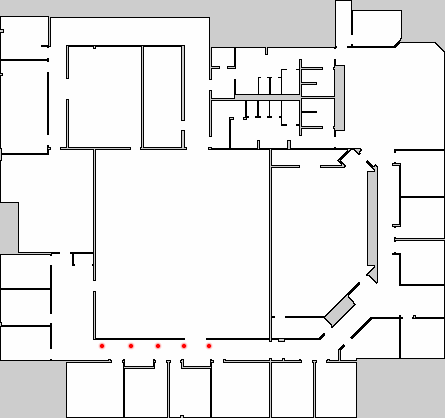
\includegraphics[width=0.5\linewidth]{imagenes/willow/0_250000mRobots2.png}
  \caption[Mapa del entorno utilizado en las pruebas.]{Mapa del entorno utilizado en las pruebas. En negro se indican las paredes, en blanco el espacio libre y en gris el espacio inaccesible. Las posiciones iniciales de los robots se indican en rojo.}
  \label{fig:willow}
\end{figure} 

El entorno fue construido a partir de un modelo que se encuentra disponible por
defecto en Gazebo, llamado \say{Willow Garage}, el cual se modifico para
reducir el area a explorar y que sea cerrado (sin salidas al exterior).

\subsection{Robots}
Los robots simulados\footnote{Especificación disponible en línea:\\
\url{https://gitlab.fing.edu.uy/federico.ciuffardi/pioneer_p3dx_model}} en las
pruebas modelan al robot diferencial Pioneer 3-DX \cite{p3dx} (figura
\ref{fig:p3dx}). Cada robot esta equipado con un sensor \gls{LiDAR} basado en el
modelo URG-04LX-UG01 \cite{hokuyo}, que permite tomar medidas de distancia de
hasta $5.6m$, utilizando una frecuencia de $10hz$ de un máximo de $36hz$.
Adicionalmente el sensor fue alterado para tomar medidas en los $360$\textdegree
al rededor del robot y para proporcionar medidas perfectas (sin ruido).

\begin{figure}[H]
  \centerfloat

  \subfloat[Real.]{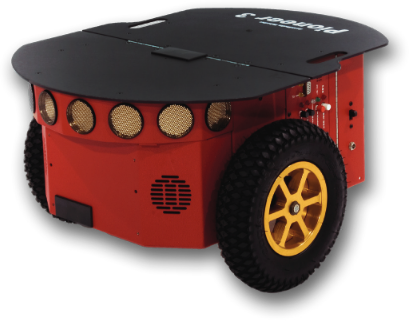
\includegraphics[clip=true, width=0.33\textwidth]{imagenes/pion/real.png}}
  \qquad
  \subfloat[Simulado.]{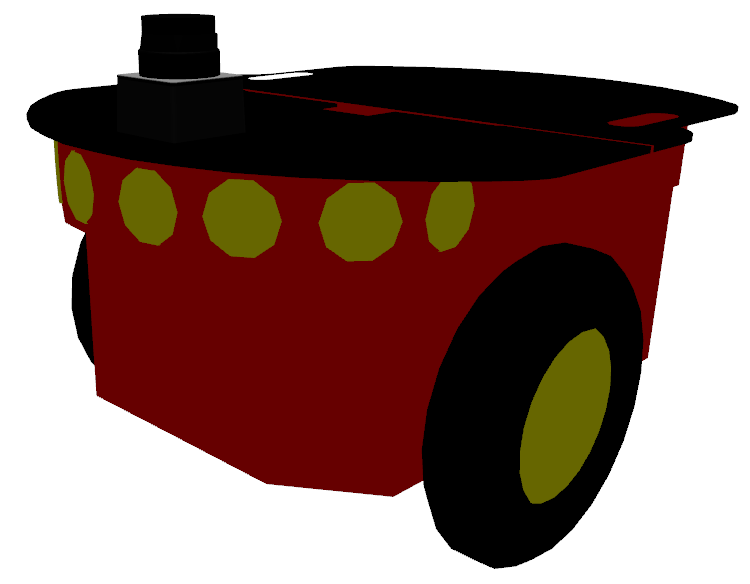
\includegraphics[clip=true, width=0.33\textwidth]{imagenes/pion/sim.png}}

  \caption[Robot diferencial Pioneer 3-DX.]{Robot diferencial Pioneer 3-DX.}\label{fig:p3dx}
   % A la izquierda se muestra el robot real, y a la derecha su version simulada.

\end{figure}

La flota de exploración se compone de cinco robots, ubicados en las posiciones
indicadas en la figura \ref{fig:willow}. Las comunicaciones entre los robots de
la flota son sin perdida y de rango infinito.

\subsection{Software}
El software utilizado en las pruebas fue Ubuntu \emph{20.04}, \gls{ROS} \emph{Noetic} y Gazebo
\emph{11.5.1}. 

\subsection{Hardware}
El simulador junto al resto de procesos necesarios para llevar a cabo una
prueba fueron ejecutados en una computadora personal equipada con un procesador
Intel Core i3-9100F, un procesador gráfico GeForce GTX 660 y 16GB de memoria
RAM.

\section{Métricas}
Con el propósito comparar cuantitativamente los resultados de las pruebas se
establece un conjunto de métricas. 

Una parte de las métricas utilizadas se proponen en \cite{yan2015metrics} y
evalúan el problema de exploración en general, estas son: \emph{tiempo de
exploración}, \emph{distancia total recorrida por la flota}, \emph{completitud
del mapa} y \emph{calidad del mapa}. 

El \emph{tiempo de exploración} refiere al tiempo desde que los robots
comienzan con la primera asignación de tareas (sección \ref{sec:asigTar}) hasta
que no se detecta más espacio desconocido por explorar y se da por terminada la exploración.

La \emph{distancia total recorrida por la flota} es la suma las distancias
recorridas por cada robot de la flota a lo largo de la exploración. En
\cite{yan2015metrics} esta métrica se presenta como \emph{costo de
exploración}, ya que los autores la consideran como una buena aproximación del
costo energético del robot. 

 % mapas de referencia para evaluar los mapas resultantes de las pruebas,

Para calcular las métricas de \emph{completitud} y \emph{calidad} de los mapas
es necesario contar con mapas de referencia considerados como correctos. En
este proyecto estos se representan a través de grillas de ocupación al igual
que los generados en la exploración. Se definen cuatro mapas de
referencia, uno por cada nivel de granularidad utilizado en las pruebas, con el
propósito de poder comparar cualquiera de los mapas obtenidos en pruebas con
un mapa de referencia de igual granularidad. Los mapas de referencia se pueden
apreciar en la figura \ref{fig:mref}. 

\begin{figure}[H]
  \centerfloat

  \subfloat[$1  \frac{celda}{m^2}$]{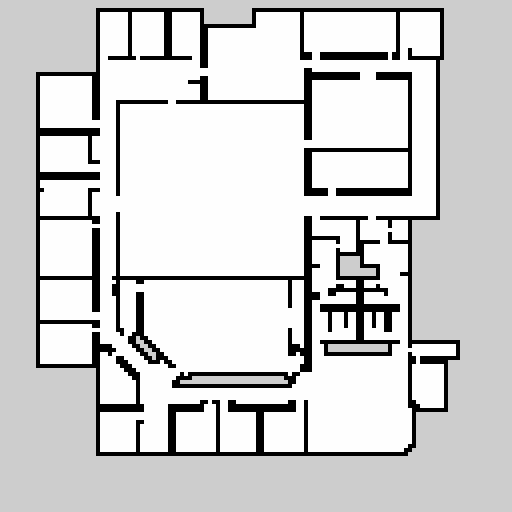
\includegraphics[clip=true, width=0.22\textwidth]{imagenes/willow_ref/1_000000m.png}}
  \qquad
  \subfloat[$4  \frac{celda}{m^2}$]{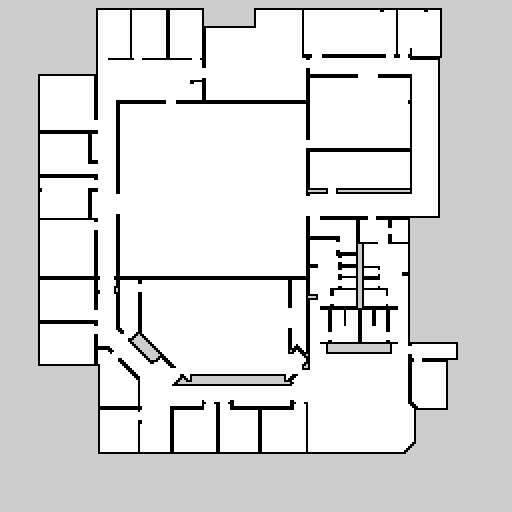
\includegraphics[clip=true, width=0.22\textwidth]{imagenes/willow_ref/0_500000m.png}}
  \qquad
  \subfloat[$9\frac{celda}{m^2}$]{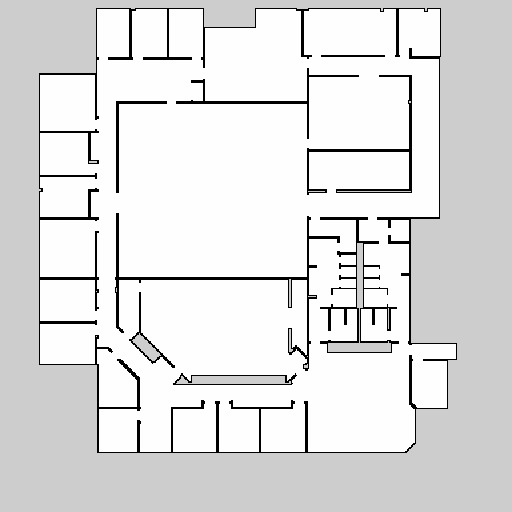
\includegraphics[clip=true, width=0.22\textwidth]{imagenes/willow_ref/0_333333m.png}}
  \qquad
  \subfloat[$16 \frac{celda}{m^2}$]{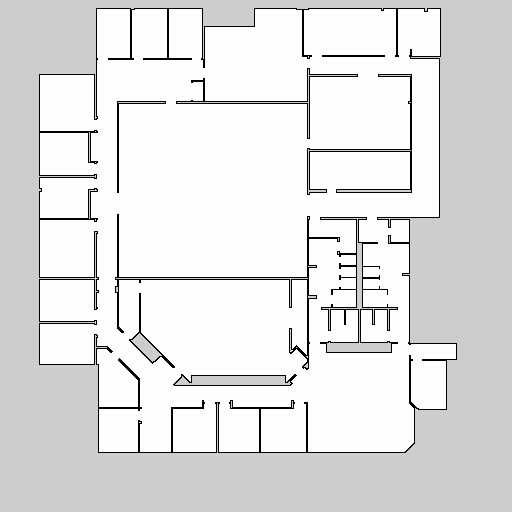
\includegraphics[clip=true, width=0.22\textwidth]{imagenes/willow_ref/0_250000m.png}}

  \caption[Mapas de referencia utilizados.]{Mapas de referencia utilizados. En negro se indican las paredes, en blanco el espacio libre y en gris el espacio desconocido por ser inaccesible.}\label{fig:mref}
   % A la izquierda se muestra el robot real, y a la derecha su version simulada.

\end{figure}

Notar que existe espacio desconocido en los mapas de referencia, esto se debe a
que la grilla de ocupación no se ajusta al espacio explorable. En términos de
las métricas calculadas, el espacio desconocido en los mapas de referencia no es
considerado como parte de los mapas, tanto en los mapas de referencia como en
los obtenidos en las pruebas.

% Es decir las unicas celdas que se consideran como
% parte de los mapas al calcular las metricas son las que tienen un estado
% distinto a desconocido en los mapas de referencia.
% De
% esta forma los mapas de referencia no contienen celdas desconocidas, a
% diferencia de los mapas resultantes de las pruebas los cuales si pueden.

La \emph{completitud del mapa} se define según (\ref{eq:metComp}) donde
$M_{exp}$ es el area conocida del mapa obtenido en la exploración y $M_{ref}$
es el area del mapa de referencia.

\begin{equation} \label{eq:metComp}
completitud\ del\ mapa = \frac{M_{exp}}{M_{ref}}
\end{equation}

La \emph{calidad del mapa} se establece en (\ref{eq:metCal}) donde se introduce
$E_{exp}$ equivalente al área ocupada por las celdas del mapa obtenido en
la exploración cuyo estado difiere del estado de su celda correspondiente en el
mapa de referencia.

\begin{equation} \label{eq:metCal}
calidad\ del\ mapa = \frac{M_{exp}-E_{exp}}{M_{ref}}
\end{equation}

El resto de las métricas fueron diseñadas específicamente para este proyecto,
estas son: \emph{tiempo promedio en construcción de GVD} y \emph{tiempo
promedio en simplificación de fronteras}.

El \emph{tiempo promedio en construcción de GVD} es el promedio del tiempo que
toma construir el GVD en las etapas de obtención de información en cada
asignación de tareas (sección \ref{sec:asigTar}).

El \emph{tiempo promedio en simplificación de fronteras} es el tiempo promedio
que se demora en simplificar las fronteras para identificar los objetivos en
cada asignación de tareas.

\section{Resultados}
\newlength{\graphlen}
\setlength{\graphlen}{0.75\textwidth}


Los resultados experimentales obtenidos son presentados y analizados en esta
sección. Las tablas que se presentan a lo largo de la sección indican para cada
prueba los promedios y desviaciones estándar de las métricas en las 20
repeticiones que se hacen debido al no determinismo del simulador.

\subsection{Cubrimiento y calidad de los mapas} \label{sec:exp:cubcal}
% Capaz aca puedo mencionar lo que pasa con los errores

% el cubrimiento y la completitud: completitud mayor a 0.999 para todas combinaciones de granularidades y soluciones probadas

% el error y la calidad:

En la tabla \ref{tab:todo3} se muestra la completitud y calidad de los mapas
obtenidos en todas las pruebas realizadas. 

Con respecto a la completitud es posible apreciar que no existen diferencias
mayores entre las variantes de la implementación, teniendo todos los mapas
generados una completitud alta. Dado que el criterio de parada es que no se
detecte más espacio por explorar, estos valores hablan principalmente de la
capacidad de detectar el espacio desconocido explorable que tienen las
soluciones. Todas las soluciones detectan espacio desconocido explorable
mientras exista una un celda $c_1$ libre y otra $c_2$ desconocida tal que $c_1
\in ady_4(c_2)$ (sección \ref{subsec:Grilla}), principalmente porque en estas
condiciones se asume que los robots no pueden atravesar de $c_1$ a $c_2$. Dicho
esto se presume que la completitud de los mapas no es perfecta debido a la
presencia de celdas ubicadas en esquinas de paredes que que a pesar de no
cumplir con las condiciones de ser detectadas como explorables, lo son. Un
ejemplo de este tipo de celda se muestra en la figura \ref{fig:faltaCub}. Sin
embargo los valores de completitud obtenidos indican que este tipo de
situaciones son despreciables.

\begin{figure}[H]
  \centerfloat

  \subfloat[Mapa de referencia.]{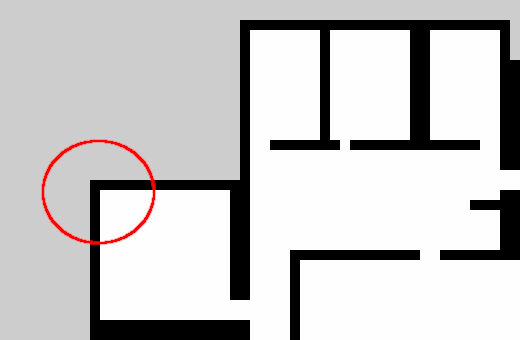
\includegraphics[clip=true, width=0.33\textwidth]{imagenes/faltaDeCub/ogred.png}}
  \qquad
  \subfloat[Mapa generado.]{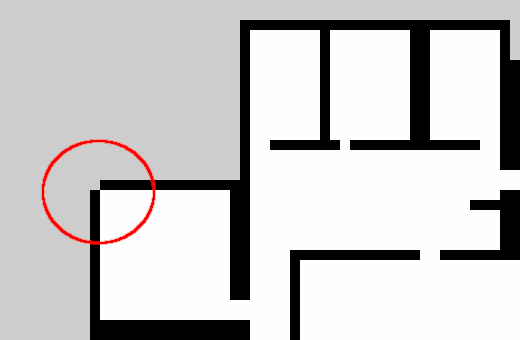
\includegraphics[clip=true, width=0.33\textwidth]{imagenes/faltaDeCub/faltaCubRed}}

  \caption{Esquina superior izquierda del mapa referencia y de uno de los mapas
  obtenidos en las pruebas que presenta una celda explorable que no se reconoce
como tal. Ambos mapas corresponden a una granularidad de una celda por metro cuadrado.}\label{fig:faltaCub}
   % A la izquierda se muestra el robot real, y a la derecha su version simulada.

\end{figure}

Los resultados de calidad de los mapas obtenidos son similares a los de
completitud, los mapas construidos tienen una calidad alta, sin existir
diferencias significativas entre las variantes. Esto es esperable ya que
los sensores simulados fueron configurados para proporcionar medidas perfectas.
Aunque a pesar de esto la calidad no perfecta, esto puede se explica en primer
lugar por el impacto de la completitud del mapa en su calidad. En segundo lugar
por la existencia de varios robots que pueden detectase como obstáculos entre
sí, generado celdas obstaculizadas que no se encuentran en el mapa de
referencia. Y en tercer lugar porque a pesar de las configuración de los
sensores, sus medidas tienen un ruido pequeño.

Estos resultados de completitud y calidad del mapa permiten concluir que todas
las variantes logran resolver de manera satisfactoria el problema de la
exploración multi-robot, en términos de los mapas construidos. Las
siguientes secciones se dedican a discutir los impactos que las diferentes
variantes en términos de tiempo y costo de exploración.


\begin{table}[H]
%29/12/2021 18:15:43
\hbadness = 10000
\tolerance=9999
\emergencystretch=10pt
\hyphenpenalty=10000
\exhyphenpenalty=100
\begin{center}

% \begin{adjustbox}{minipage=0.75\paperwidth, center}
\begin{adjustbox}{width=1\textwidth}
\small

\begin{tabularx}{\textwidth}{|X|C{0.80cm}|X|X|}

\hline
Variante & $\frac{celdas}{m^2}$ & Completitud del mapa & Calidad del mapa \\ \hline\hline
\multirow{4}{\linewidth}{\centering Propuesta sin cambios}
& 1 & 0.999725±1.5e-04 & 0.999039±3.1e-04\\ \cline{2-4}
& 4 & 0.999925±6.5e-05 & 0.999703±1.7e-04\\ \cline{2-4}
& 9 & 0.999983±1.2e-05 & 0.999858±5.7e-05\\ \cline{2-4}
& 16 & 0.999998±3.6e-06 & 0.999929±3.4e-05\\ \hline\hline
\multirow{4}{\linewidth}{\centering No incremental}
& 1 & 0.999763±8.9e-05 & 0.999208±2.2e-04\\ \cline{2-4}
& 4 & 0.999957±4.2e-05 & 0.999805±1.3e-04\\ \cline{2-4}
& 9 & 0.999984±1.6e-05 & 0.999864±4.7e-05\\ \cline{2-4}
& 16 & 0.999999±1.9e-06 & 0.999941±3.3e-05\\ \hline\hline
\multirow{4}{\linewidth}{\centering Simplificación de fronteras basada en K-Means}
& 1 & 0.999802±1.3e-04 & 0.999179±2.8e-04\\ \cline{2-4}
& 4 & 0.999977±2.7e-05 & 0.999767±8.0e-05\\ \cline{2-4}
& 9 & 0.999976±2.3e-05 & 0.999831±7.4e-05\\ \cline{2-4}
& 16 & 0.999999±2.5e-06 & 0.999930±1.8e-05\\ \hline\hline
\multirow{4}{\linewidth}{\centering Fronteras sin simplificar}
& 1 & 0.999937±7.6e-05 & 0.999493±2.0e-04\\ \cline{2-4}
& 4 & 0.999995±9.8e-06 & 0.999837±4.8e-05\\ \cline{2-4}
& 9 & 0.999983±4.0e-05 & 0.999729±7.6e-05\\ \cline{2-4}
& 16 & 0.999998±4.1e-06 & 0.999921±2.2e-05\\ \hline\hline
\multirow{4}{\linewidth}{\centering Desconocidas se consideran libres}
& 1 & 0.999812±1.1e-04 & 0.999256±3.2e-04\\ \cline{2-4}
& 4 & 0.999972±1.9e-05 & 0.999786±9.7e-05\\ \cline{2-4}
& 9 & 0.999987±1.2e-05 & 0.999840±6.9e-05\\ \cline{2-4}
& 16 & 0.999998±3.5e-06 & 0.999940±2.8e-05\\ \hline
\end{tabularx}
\end{adjustbox}

\caption{Completitud y calidad de los mapas obtenidos en todas las pruebas realizadas.}
\label{tab:todo3}
\end{center}

\end{table}


\subsection{Incrementalidad}\label{sec:exp:inc}
En esta sección se comparan los resultados de las pruebas realizadas con
solución propuesta que construye el GVD de forma incremental contra los de una
variante que solo difiere en que la construcción del GVD es no incremental. Las
métricas a analizar para estas pruebas se encuentran en la tabla \ref{tab:inc1}
y graficadas en las figuras \ref{fig:gra:inc:et}, \ref{fig:gra:inc:ec} y
\ref{fig:gra:inc:gvdt}.

En cada nivel de granularidad la variante incremental reduce un
${\smallsim}94\%$ el tiempo promedio construcción del GVD con respecto a la
variante no incremental. Esto valida la idea de que la construcción incremental
del GVD es más eficiente que su contraparte no incremental.

% El tiempo de construcción de GVD impacta directamente al tiempo que ocurre
% desde que un robot pide un tarea y una le es asignada, ya que es una parte
% necesaria y no paralelizada de la etapa de obtención de información (sección
% \ref{subsec:obtInfo}) de cada asignación de tareas (sección \ref{sec:asigTar}).
% A pesar de esto el impacto sobre los tiempos de exploración no es directo. Esto
% se debe al hecho de que una asignación de tareas este en curso solo asegura que un único
% robot estara osicoso, ya que mientras que un robot pide una tarea y la obitene
% el resto puede estar completando tareas asignadas previamente. Cuanto más corta 
% es la demora en la asignación de tareas más probable es que un único robot quede
% osicoso, mientras que si dicha demora aumenta, también lo hace la probabilidad
% que en el transcurso de la asignacion más robots completen sus tareas y
% requieran tareas, quedando ociosos. Esto logra explicar que en todos los
% niveles de granularidad la reduccion del tiempo promedio logrado por la
% variante incremental frente a la no incremental sea de un ${\smallsim}94\%$
% constante mientras que la reduccion del tiempo de exploración comienza siendo
% de un ${\smallsim}8\%$ en el nivel de granularidad más bajo (tiempos de
% construcción de GVD más altos), creciendo mediante se aumenta el nivel de
% granularidad llegando a una reduccion de un ${\smallsim}63\%$ en la
% granularidad más alta (tiempos de construcción de
% GVD más altos).

Con respecto a los tiempos de exploración, estos también son reducidos al
construir el GVD de forma incremental. La reducción comienza siendo de un
${\smallsim}8\%$ en el nivel de granularidad más bajo, y mediante se aumenta el
nivel de granularidad las reducciones también aumentan hasta llegar a una
reducción de ${\smallsim}63\%$ en el nivel más alto. Esto se explica porque el
tiempo de construcción de GVD impacta directamente al tiempo que ocurre desde
que un robot pide un tarea y una le es asignada, por ser una parte necesaria y
no paralelizada de la etapa de obtención de información (sección
\ref{subsec:obtInfo}) de cada asignación de tareas (sección \ref{sec:asigTar}).
Y los tiempos de asignación de tareas impactan a los tiempos de exploración,
pero en este caso el impacto no es directo. Esto se debe a que una asignación
de tareas en curso solo asegura que un único robot esta ocioso, porque
mientras que un robot pide una tarea y una le es asignada el resto puede estar
completando tareas asignadas previamente. Cuanto más corta es la demora en la
asignación de tareas más probable es que un único robot quede ocioso, mientras
que si dicha demora aumenta, también lo hace la probabilidad que en el
transcurso de la asignación más robots completen sus tareas y requieran tareas,
quedando ociosos. 
% no son
% monótonamente crecientes ni decrecientes respecto a la granularidad

% las reducciones no son significativas. Especificamente, 
% y adicionalmente las diferencias entre los promedios de
% esta metrica son similares a sus desviaciones estándar

Construir el GVD de forma incremental también parece reducir las distancias
totales recorridas por la flota en todas las granularidades, aunque en este
caso las reducciones están comprendidas entre $2\%$ y $7\%$, fluctuando al
aumentar los niveles de granularidad. Esto puede deberse a que tiempos más
rápidos de asignación de objetivos hacen más probable que los robots cambien su
trayectoria a un nuevo objetivo antes de llegar a la ubicación exacta del
objetivo previamente completado. Esto puede reducir la distancia recorrida por
el robot si los caminos hacia el objetivo anterior y el actual no se solapan.

% En cada nivel de granularidad el tiempo promedio en construcción del GVD de
% variante incremental siempre es menor que el de la variante no incremental,
% aumentando la diferencia a medida que aumentan las celdas por metro cuadrado.
% La reducción del tiempo tiempo de construcción del GVD que se logra al

% construirlo de forma incremental implica una reducción del $55\%$ en el
% porcentaje de tiempo de la obtención de información en la que se construye el
% GVD aproximadamente que se repite en todos los niveles de granularidad.

% Como los tiempos de construcción promedio del GVD son menores
% en las pruebas realizadas con las construcción incremental del GVD,

% al aumentar las celdas por metro cuadrado, el tiempo
% promedio en construcción del GVD, en el caso de la construcción incremental crece de a 

\begin{table}[H]
%29/12/2021 18:15:42
\hbadness = 10000
\tolerance=9999
\emergencystretch=10pt
\hyphenpenalty=10000
\exhyphenpenalty=100
\begin{center}

% \begin{adjustbox}{minipage=0.75\paperwidth, center}
\begin{adjustbox}{width=1\textwidth}
\small

\begin{tabularx}{\textwidth}{|X|C{0.80cm}|X|X|X|}

\hline
Construcción del GVD & $\frac{celdas}{m^2}$ & Tiempo de exploración $(s)$ & Distancia total recorrida por la flota $(m)$ & Tiempo promedio en construcción de GVD $(s)$ \\ \hline\hline
\multirow{4}{\linewidth}{\centering Incremental}
& 1 & 463.0±22.6 & 2480.5±109.7 & 0.0442±0.0017\\ \cline{2-5}
& 4 & 496.4±19.0 & 2745.2±107.3 & 0.1762±0.0057\\ \cline{2-5}
& 9 & 549.2±18.4 & 2849.3±95.2 & 0.4204±0.0174\\ \cline{2-5}
& 16 & 678.4±24.8 & 3050.3±105.2 & 0.7641±0.0334\\ \hline\hline
\multirow{4}{\linewidth}{\centering No incremental}
& 1 & 501.9±22.4 & 2653.4±96.5 & 0.7199±0.0122\\ \cline{2-5}
& 4 & 745.7±23.1 & 2851.1±144.0 & 2.8603±0.0484\\ \cline{2-5}
& 9 & 1198.7±35.8 & 3038.1±159.2 & 6.8253±0.1713\\ \cline{2-5}
& 16 & 1856.7±56.2 & 3117.0±170.3 & 12.9256±0.3056\\ \hline
\end{tabularx}
\end{adjustbox}

\caption{Resultados obtenidos en las pruebas realizadas con la construcción incremental y no incremental del GVD.}
\label{tab:inc1}
\end{center}

\end{table}
\todo[inline]{cuadro 4.2: qué tal, Construcción del GVD: incremental vs no incremental}



\begin{figure}[H]
  \centerfloat

  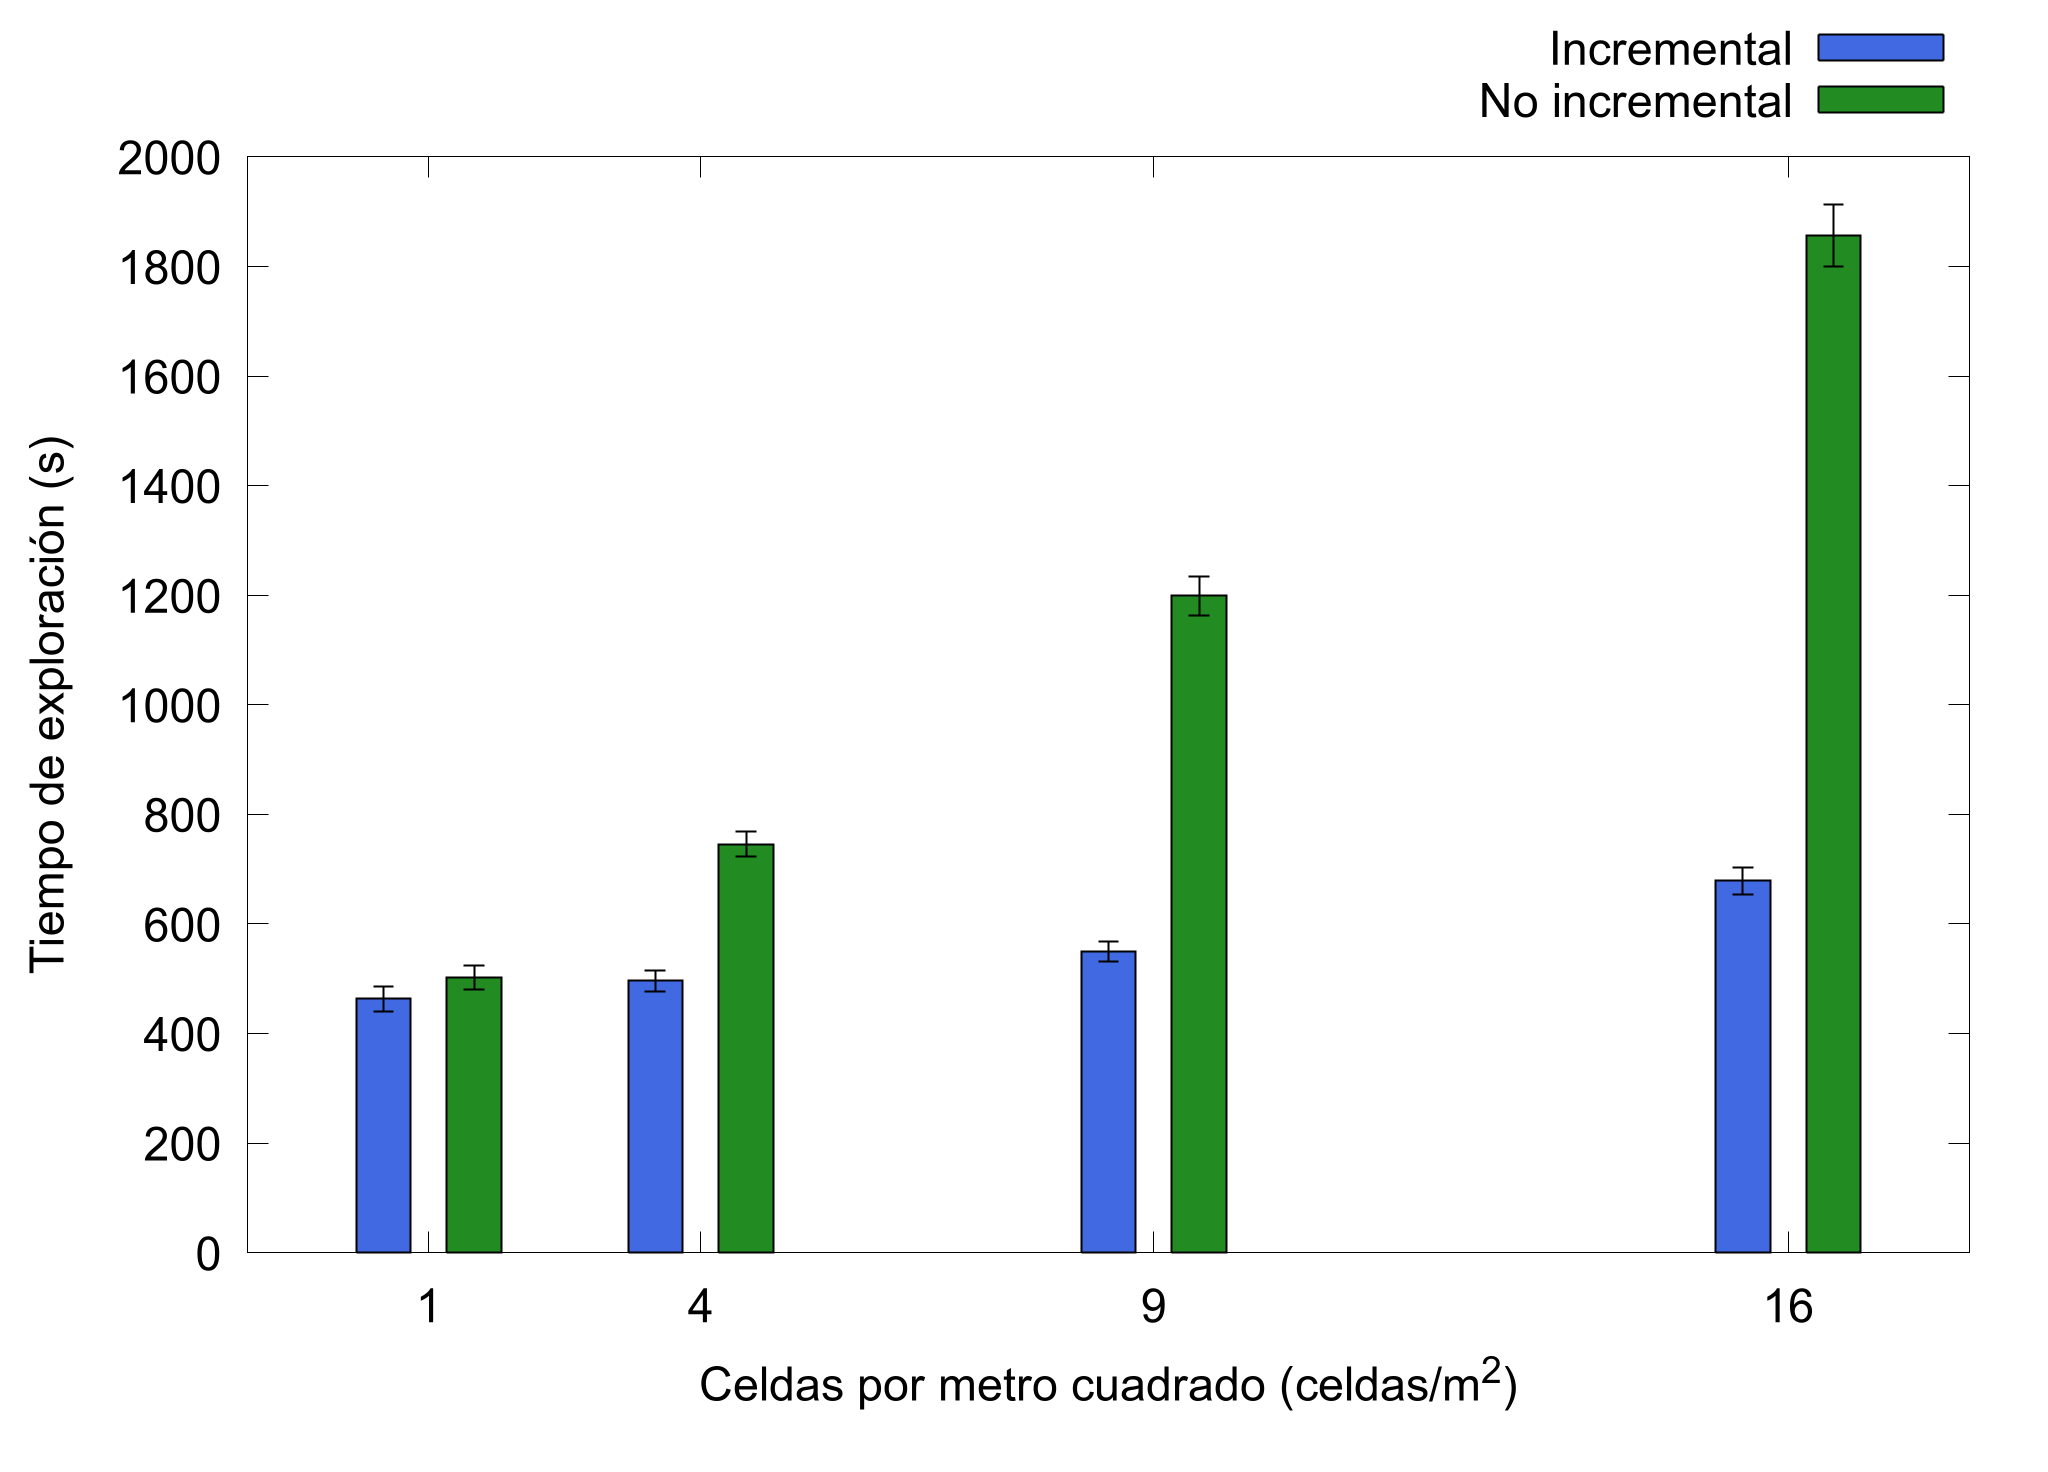
\includegraphics[clip=true, width=\graphlen]{imagenes/graficas_chicas/graficas_histo_num/incrementalidad/exploration_time.png}

  \caption{Gráfica de tiempo de exploración en función de celdas por metro cuadrado.}\label{fig:gra:inc:et}

\end{figure}

\begin{figure}[H]
  \centerfloat

  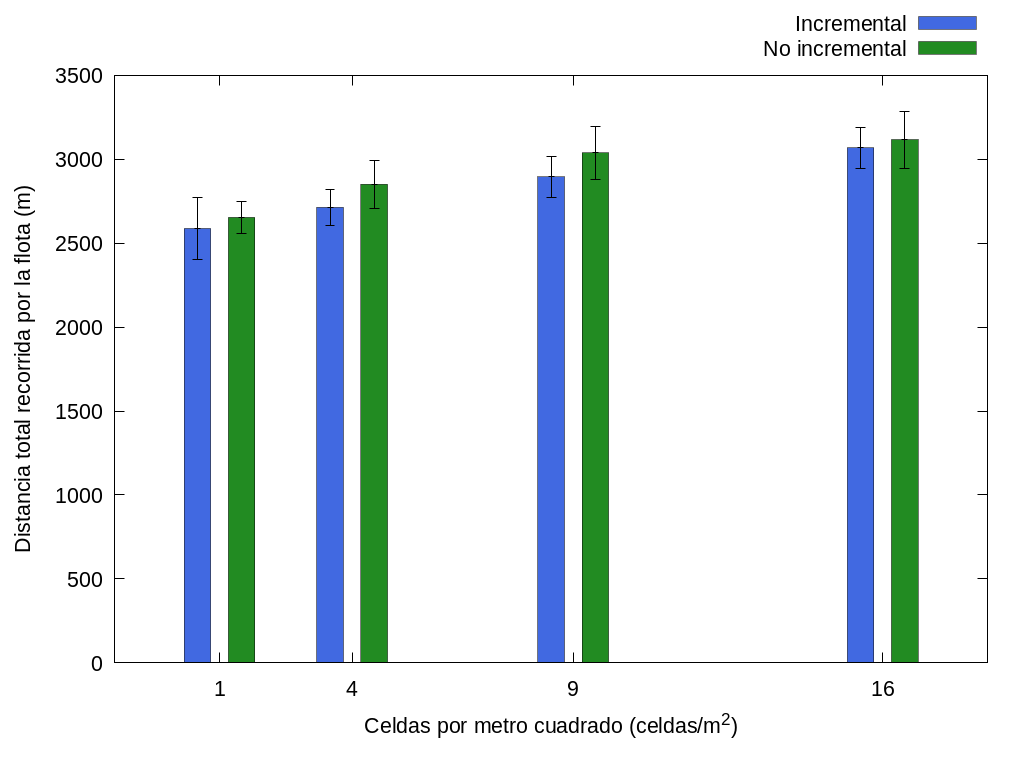
\includegraphics[clip=true, width=\graphlen]{imagenes/graficas_chicas/graficas_histo_num/incrementalidad/exploration_cost.png}

  \caption{Gráfica de distancia total recorrida por la flota  en función de celdas por metro cuadrado.}\label{fig:gra:inc:ec}

\end{figure}

\begin{figure}[H]
  \centerfloat

  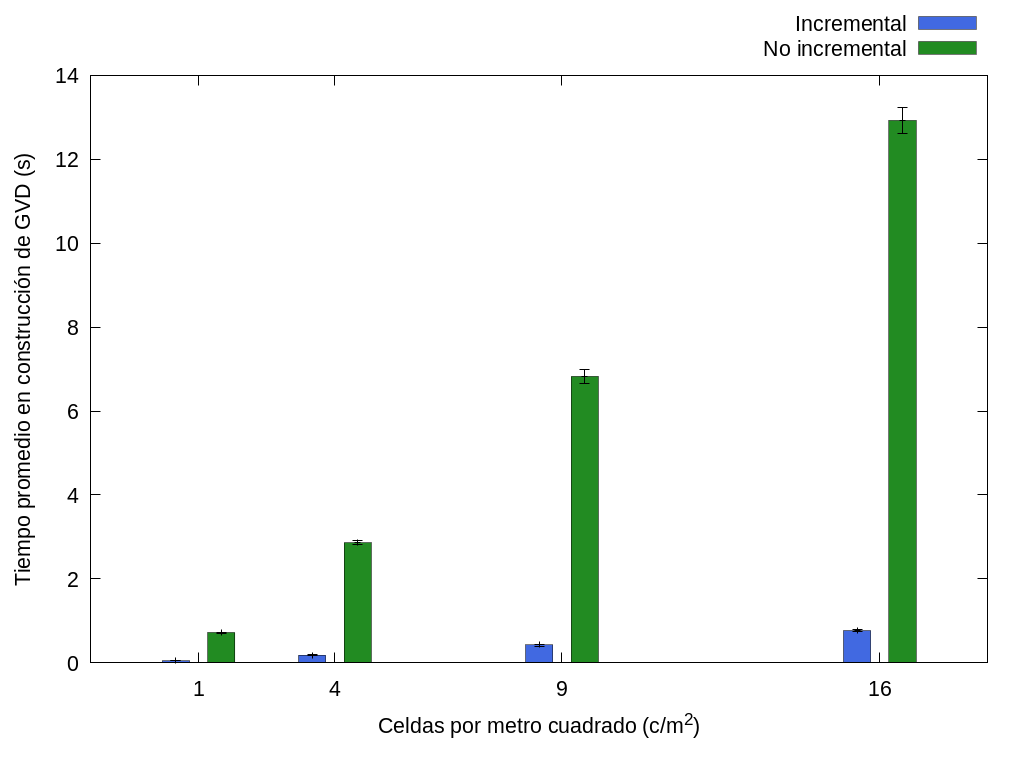
\includegraphics[clip=true, width=\graphlen]{imagenes/graficas_chicas/graficas_histo_num/incrementalidad/gvd_construction_time_mean.png}

  \caption{Gráfica del tiempo promedio en construcción de GVD en función de celdas por metro cuadrado.}\label{fig:gra:inc:gvdt}

\end{figure}


\subsection{Identificación de objetivos}\label{sec:exp:idobj}
En esta sección se realiza un análisis comparativo de los resultados obtenidos
en pruebas realizadas con tres soluciones distintas que difieren únicamente en
el método usado para identificar objetivos (sección \ref{sec:pc:idobj}). Estos
métodos son: la simplificación de fronteras basada en cubrimiento propuesta en
este proyecto, simplificación de fronteras basada en K-Means como es utilizada en
\cite{Amorin2019} y la identificación de fronteras (sin simplificar)
introducida en \cite{yamauchi1998frontier}. Los resultados de las métricas a
analizar se presentan en la tabla \ref{tab:inc1} y se encuentran graficadas en
las figuras \ref{fig:gra:inc:et}, \ref{fig:gra:inc:ec} y
\ref{fig:gra:inc:gvdt}.

Es posible apreciar que los métodos que identifican los objetivos simplificando
las fronteras reducen los tiempos de exploración con respecto al método que
identifica a las fronteras sin simplificar como objetivos. Aunque en el nivel
de granularidad más bajo las reducciones son menores a ${\smallsim}5\%$, estas crecen junto
a la granularidad hasta alcanzarse una reducción de ${\smallsim}29\%$ en el
nivel más alto. Esto puede deberse al tiempo de asignación de tareas como se
explica en la sección \ref{sec:exp:inc}. En este caso se considera que los
factores con mayor impacto sobre los tiempos de asignación de tareas son dos:
el tiempo de simplificación de fronteras y la cantidad de objetivos
identificados. Mayores tiempos de simplificación fronteras retrasan la
identificación de objetivos, parte necesaria y no paralelizada de la etapa de
obtención de información (sección \ref{subsec:obtInfo}) en la asignación de
tareas. Mientras que disminuir la cantidad de objetivos identificados implica
reducciones en la duración de las etapas de valuación (sección
\ref{subsec:MiValSub}) y de resolución (sección \ref{subsec:MiResSub}) al ser
menor la cantidad de objetivos a valuar y a considerar en la resolución. Entonces lo que se evidencia
en los resultados obtenidos, es que invertir tiempo en disminuir los objetivos
identificados simplificando las fronteras lleva a una reducción total de los
tiempos de asignación de tareas, y en consecuencia de los tiempos de exploración
frente a no invertir dicho tiempo y utilizar todas las fronteras sin
simplificar. Otra razón posible para las reducciones del tiempo de exploración
es que simplificar las fronteras puede aportar a la coordinación de los robots.
Por ejemplo de no simplificarse las fronteras se permite que un robot sea
asignado a un objetivo adyacente a una pared o que dos robots sean asignados a
objetivos adyacentes entre sí, situaciones en las cuales se desaprovecha
capacidad de sensado, y se complejizó la navegación. Al simplificarse las
fronteras, especialmente cuando se logra el cubrimiento minimizando los
objetivos resultantes, se evitan situaciones como las descritas lo cual puede
verse como una coordinación pasiva. \todo{o implicita?}

De acuerdo con los resultados simplificar las fronteras en la identificación de
objetivos también reduce las distancias totales recorridas por la flota frente
a no simplificarlas. Estas reducciones son en general de ${\smallsim}10\%$, y
pueden ser causadas por la disminución del tiempo de asignación de tareas,
debido a las mismas razones que se explican en la sección \ref{sec:exp:inc}.
Aunque la coordinación pasiva también puede estar jugando un rol al evitar que
los robots se trasladen a objetivos que desaprovechan las capacidades
sensoriales del robot o que puedan llevar a inconvenientes en la navegación.

Con respecto a los dos métodos que simplifican las fronteras para 
identificar objetivos, en el nivel de granularidad más bajo, la
simplificación basada en cubrimiento logra una reducción con respecto a la
basada en K-Means de ${\smallsim}3\%$ en la distancia total recorrida por la
flota y de ${\smallsim}5\%$ en los tiempo de exploración. Esto se invierte a
medida que aumenta el nivel de granularidad, hasta que en el nivel más alto en
lugar de reducirse, las métricas aumentan. La distancia total recorrida por la
flota aumenta en un ${\smallsim}3\%$ y el tiempo de exploración en un
${\smallsim}6\%$. Por otro lado según los resultados obtenidos del tiempo
promedio en simplificación de fronteras, la simplificación basada en
cubrimiento en todo nivel de granularidad es entre $2$ y
$4$ veces más lenta que la basada en K-Means. Estos resultados
parecen indicar que la simplificación basada en cubrimiento toma más tiempo
pero logra mejores reducciones de objetivos que la basada en K-Means. En el
nivel de granularidad más bajo el aumento de tiempo de simplificación no es tan
relevante como la reducción de objetivos, por lo tanto la simplificación basada
en cubrimiento obtiene un mejor rendimiento. A medida la granularidad crece el
aumento de tiempo de simplificación se torna más relevante que la reducción de
objetivos, por lo que la simplificación basada en K-Means obtiene un
rendimiento superior.  

\begin{table}[H]
%24/12/2021 03:06:43
\hbadness = 10000
\tolerance=9999
\emergencystretch=10pt
\hyphenpenalty=10000
\exhyphenpenalty=100
\begin{center}

% \begin{adjustbox}{minipage=0.75\paperwidth, center}
\begin{adjustbox}{width=1\textwidth}
\small

\begin{tabularx}{\textwidth}{|X|C{0.80cm}|X|X|}

\hline
Identificación de objetivos & $\frac{celdas}{m^2}$ & Tiempo de exploración $(s)$ & Distancia total recorrida por la flota $(m)$ \\ \hline\hline
\multirow{4}{\linewidth}{\centering Simplificación de fronteras basada en cubrimiento}
& 1 & 480.8±34.7 & 2587.0±186.4\\ \cline{2-4}
& 4 & 498.0±25.3 & 2713.1±107.5\\ \cline{2-4}
& 9 & 553.4±24.9 & 2894.7±124.5\\ \cline{2-4}
& 16 & 689.7±29.0 & 3067.9±121.9\\ \hline\hline
\multirow{4}{\linewidth}{\centering Simplificación de fronteras basada en K-Means}
& 1 & 491.0±25.7 & 2628.0±98.6\\ \cline{2-4}
& 4 & 494.3±28.2 & 2684.8±106.7\\ \cline{2-4}
& 9 & 532.6±21.1 & 2813.0±96.4\\ \cline{2-4}
& 16 & 652.0±32.7 & 2962.4±136.6\\ \hline\hline
\multirow{4}{\linewidth}{\centering Fronteras sin simplificar}
& 1 & 487.9±24.3 & 2750.7±142.3\\ \cline{2-4}
& 4 & 532.8±24.7 & 3028.3±136.1\\ \cline{2-4}
& 9 & 643.3±22.8 & 3216.9±121.3\\ \cline{2-4}
& 16 & 925.8±104.7 & 3352.5±208.7\\ \hline
\end{tabularx}
\end{adjustbox}

\caption{Resultados de tiempo y costo de exploración obtenidos en las pruebas realizadas con los distintos métodos de identificación de objetivos.}
\label{tab:ident_obj1}
\end{center}

\end{table}


\begin{figure}[H]
  \centerfloat

  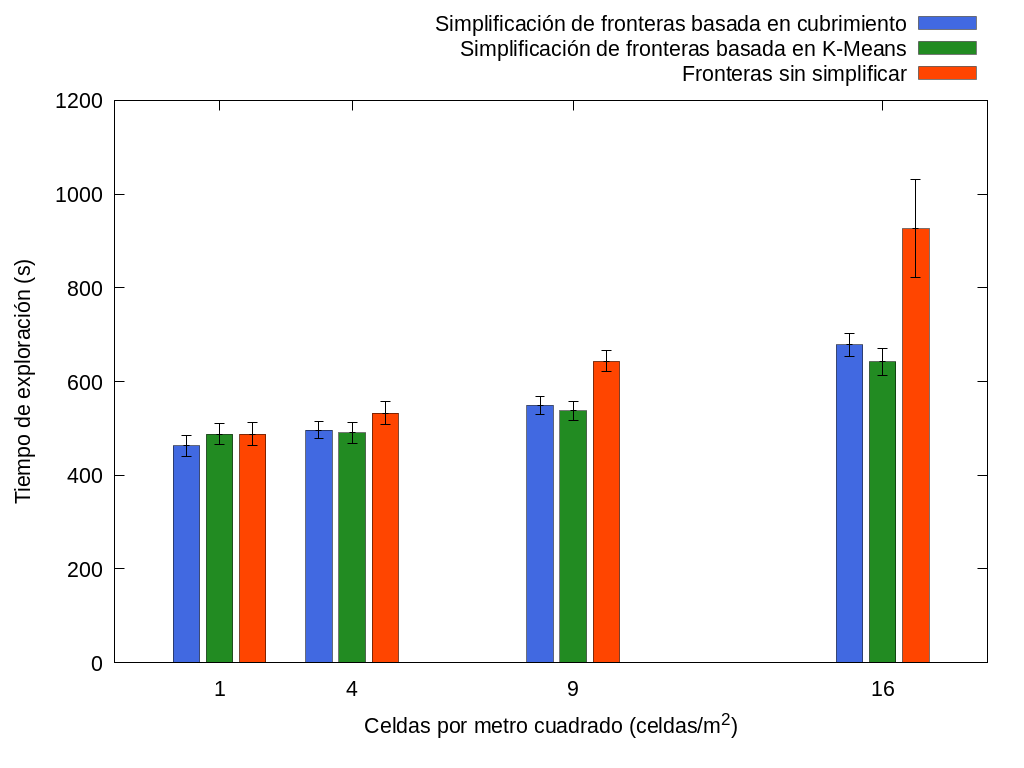
\includegraphics[clip=true, width=\graphlen]{imagenes/graficas_chicas/graficas_histo_num/ident_obj/exploration_time.png}

  \caption{Gráfica de tiempo de exploración en función de celdas por metro cuadrado.}\label{fig:gra:idobj:et}

\end{figure}

\begin{figure}[H]
  \centerfloat

  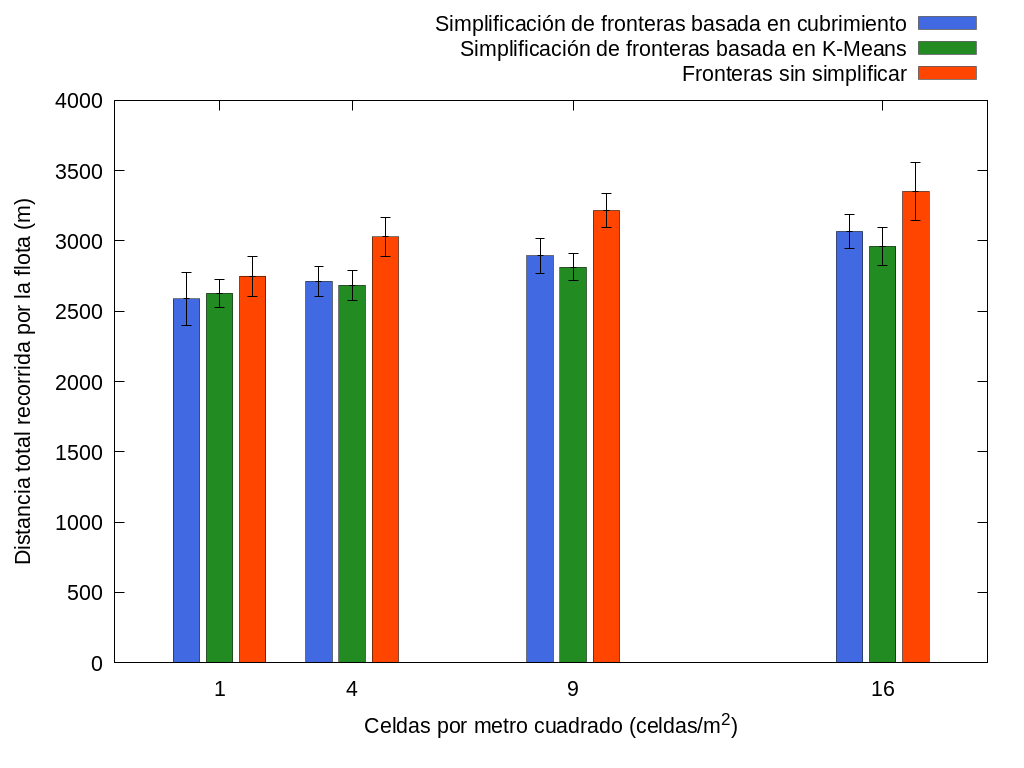
\includegraphics[clip=true, width=\graphlen]{imagenes/graficas_chicas/graficas_histo_num/ident_obj/exploration_cost.png}

  \caption{Gráfica de distancia total recorrida por la flota en función de celdas por metro cuadrado.}\label{fig:gra:idobj:ec}

\end{figure}

\begin{figure}[H]
  \centerfloat

  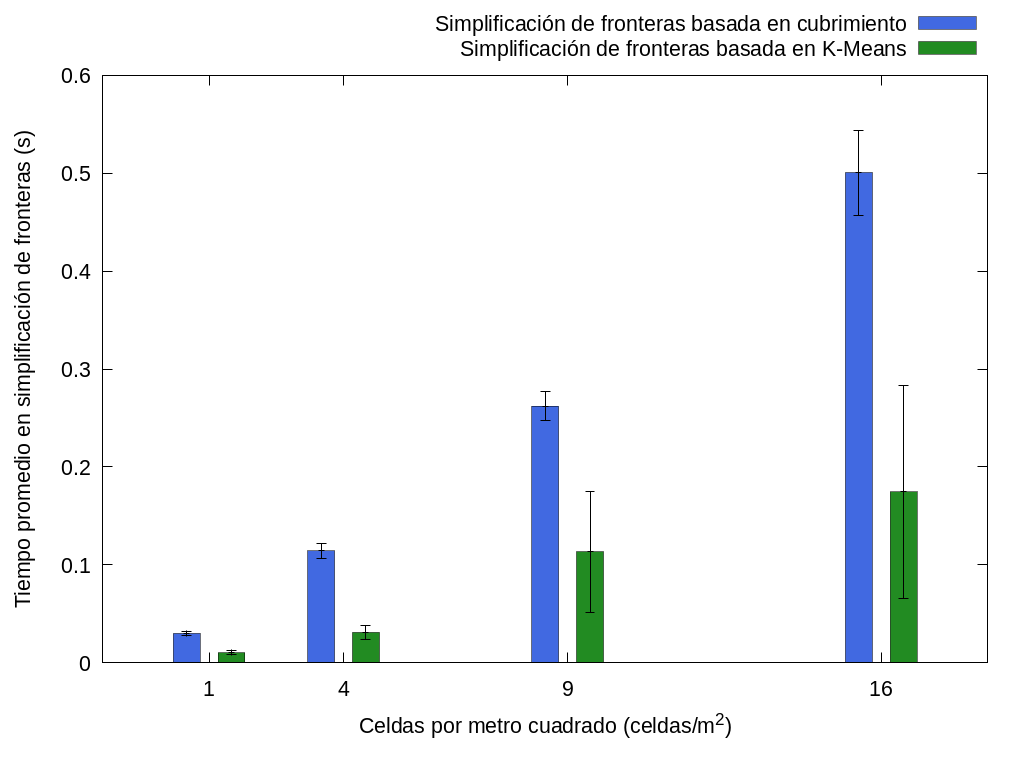
\includegraphics[clip=true, width=\graphlen]{imagenes/graficas_chicas/graficas_histo_num/ident_obj/obj_id_time_mean.png}

  \caption{Gráfica del tiempo promedio en obtención de información función de celdas por metro cuadrado.}\label{fig:gra:idobj:iobt}

\end{figure}

\subsection{Consideración del espacio desconocido}\label{sec:exp:desco}

Las pruebas analizadas en esta sección corresponden a las realizadas con
soluciones que varían únicamente en la forma de considerar el espacio
desconocido al construir el GVD. Dichas formas son dos: considerar las
celdas desconocidas como libres y considerar que las celdas desconocidas no
propagan olas y que el conjunto $\mli{UF}$ de celdas desconocidas que son
adyacentes a celdas conocidas pertenecen a generadores ($\mli{UF} \subseteq
\mli{CGen}$). Ambas son descritas en la sección \ref{subsec:espDesc}. Los
resultados obtenidos en estas pruebas exponen en la tabla \ref{tab:inc1} y sus
gráficas en las figuras \ref{fig:gra:inc:et}, \ref{fig:gra:inc:ec} y
\ref{fig:gra:inc:gvdt}.

Considerar que las celdas desconocidas no propagan olas y que $\mli{UF}
\subseteq \mli{CGen}$ logra una reducción de ${\smallsim}61\%$ en el tiempo
promedio de construcción del GVD en cada nivel de granularidad, respecto a
considerar a las celdas desconocidas como libres. Estos resultados validan que
restringir la construcción del GVD al espacio conocido lleva a mejoras en los
tiempos de construcción del GVD. 


Adicionalmente tanto el tiempo de exploración como las distancias totales
recorridas por las flota son reducidas al considerar que las celdas
desconocidas no propagan olas y que $\mli{UF} \subseteq \mli{CGen}$. La
reducción del tiempo de exploración comienza siendo de ${\smallsim}3\%$ en el
nivel de granularidad más bajo, llegando a una reducción de ${\smallsim}29\%$
en el nivel más alto. Mientras que la reducción de la distancia total recorrida
por la flota fluctúa entre ninguna reducción y una reducción de
${\smallsim}9\%$. Esto puede ser causado porque la reducción de los tiempos de
construcción del GVD implica una reducción en los tiempos de asignación de
tareas y esto último se asocia a reducciones en los tiempos de exploración y de
las distancias totales recorridas por la flota, como se explica en la sección
\ref{sec:exp:inc} donde se compara la construcción incremental y no incremental
del GVD. Aunque en este caso las reducciones de los tiempos de construcción del
GVD son menores y por lo tanto los efectos sobre las métricas son menos
pronunciados. A su vez, considerar el espacio desconocido de distinta manera
cambia significativamente la forma del GVD lo cual también puede afectar a los
caminos de los robots sobre este y por lo tanto a las métricas en cuestión.


% Con respecto a los tiempos de exploración, estos tambien son reducidos al
% contruir el GVD de forma incremental. La reducción comienza siendo de un
% ${\smallsim}8\%$ en el nivel de granularidad más bajo, y mediante se aumenta el
% nivel de granularidad las reducciones tambien aumentan hasta llegar a una
% reducción de ${\smallsim}63\%$ en el nivel más alto. Esto se explica porque el
% tiempo de construcción de GVD impacta directamente al tiempo que ocurre desde
% que un robot pide un tarea y una le es asignada, por ser una parte necesaria y
% no paralelizada de la etapa de obtención de información (sección
% \ref{subsec:obtInfo}) de cada asignación de tareas (sección \ref{sec:asigTar}).
% Y los tiempos de asignación de tareas impactan a los tiempos de exploración,
% pero en este caso el impacto no es directo. Esto se debe a que una asignación
% de tareas en curso solo asegura que un único robot esta osicoso, porque
% mientras que un robot pide una tarea y una le es asignada el resto puede estar
% completando tareas asignadas previamente. Cuanto más corta es la demora en la
% asignación de tareas más probable es que un único robot quede osicoso, mientras
% que si dicha demora aumenta, también lo hace la probabilidad que en el
% transcurso de la asignacion más robots completen sus tareas y requieran tareas,
% quedando ociosos. 
% no son
% monótonamente crecientes ni decrecientes respecto a la granularidad

% las reducciones no son significativas. Especificamente, 
% y adicionalmente las diferencias entre los promedios de
% esta metrica son similares a sus desviaciones estándar

% Construir el GVD de forma incremental también parece reducir las distancias
% totales recorridas por la flota en todas las granularidades, aunque en este
% caso las reducciones estan comprendidas entre $2\%$ y $7\%$, fluctuando al
% aumentar los niveles de granularidad. Esto puede deberse a que tiempos más
% rapidos de asignación de objetivos hacen más probable que los robots cambien su
% trayectoria a un nuevo objetivo antes de llegar a la ubicación exacta del
% objetivo previamente completado. Esto puede reducir la distancia recorrida por
% el robot si los caminos hacia el objetivo anterior y el actual no se solapan.




\begin{table}[H]
%24/12/2021 03:06:43
\hbadness = 10000
\tolerance=9999
\emergencystretch=10pt
\hyphenpenalty=10000
\exhyphenpenalty=100
\begin{center}

% \begin{adjustbox}{minipage=0.75\paperwidth, center}
\begin{adjustbox}{width=1\textwidth}
\small

\begin{tabularx}{\textwidth}{|X|C{0.80cm}|X|X|}

\hline
Consideración del espacio desconocido & $\frac{celdas}{m^2}$ & Tiempo de exploración $(s)$ & Distancia total recorrida por la flota $(m)$ \\ \hline\hline
\multirow{4}{\linewidth}{\centering Desconocidas no propagan olas y $UF \subseteq CGen$}
& 1 & 480.8±34.7 & 2587.0±186.4\\ \cline{2-4}
& 4 & 498.0±25.3 & 2713.1±107.5\\ \cline{2-4}
& 9 & 553.4±24.9 & 2894.7±124.5\\ \cline{2-4}
& 16 & 689.7±29.0 & 3067.9±121.9\\ \hline\hline
\multirow{4}{\linewidth}{\centering Desconocidas se consideran libres}
& 1 & 479.1±34.4 & 2522.2±149.5\\ \cline{2-4}
& 4 & 510.5±27.1 & 2728.9±135.2\\ \cline{2-4}
& 9 & 677.8±26.4 & 3134.2±148.8\\ \cline{2-4}
& 16 & 955.4±42.1 & 3303.6±240.5\\ \hline
\end{tabularx}
\end{adjustbox}

\caption{Resultados de tiempo y costo de exploración obtenidos en las pruebas realizadas con las distintas consideraciones del espacio desconocido al construir el GVD.}
\label{tab:desconocido1}
\end{center}

\end{table}


\begin{figure}[H]
  \centerfloat

  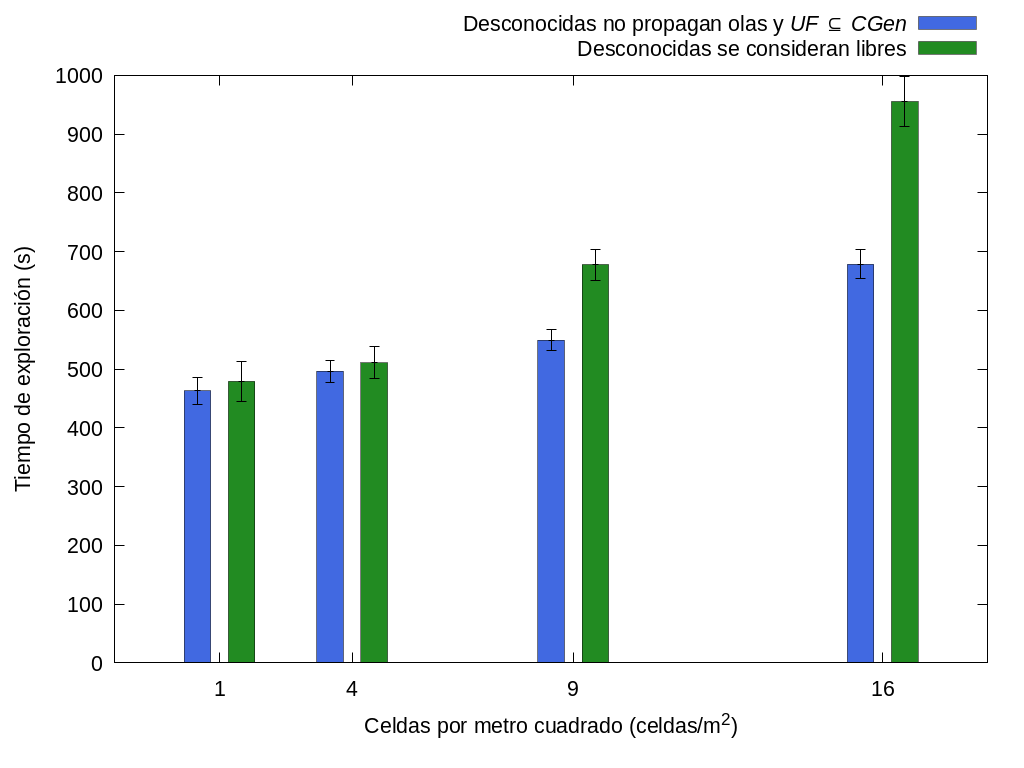
\includegraphics[clip=true, width=\graphlen]{imagenes/graficas_chicas/graficas_histo_num/desconocido/exploration_time.png}

  \caption{Gráfica de tiempo de exploración en función de celdas por metro cuadrado.}\label{fig:gra:des:et}

\end{figure}

\begin{figure}[H]
  \centerfloat

  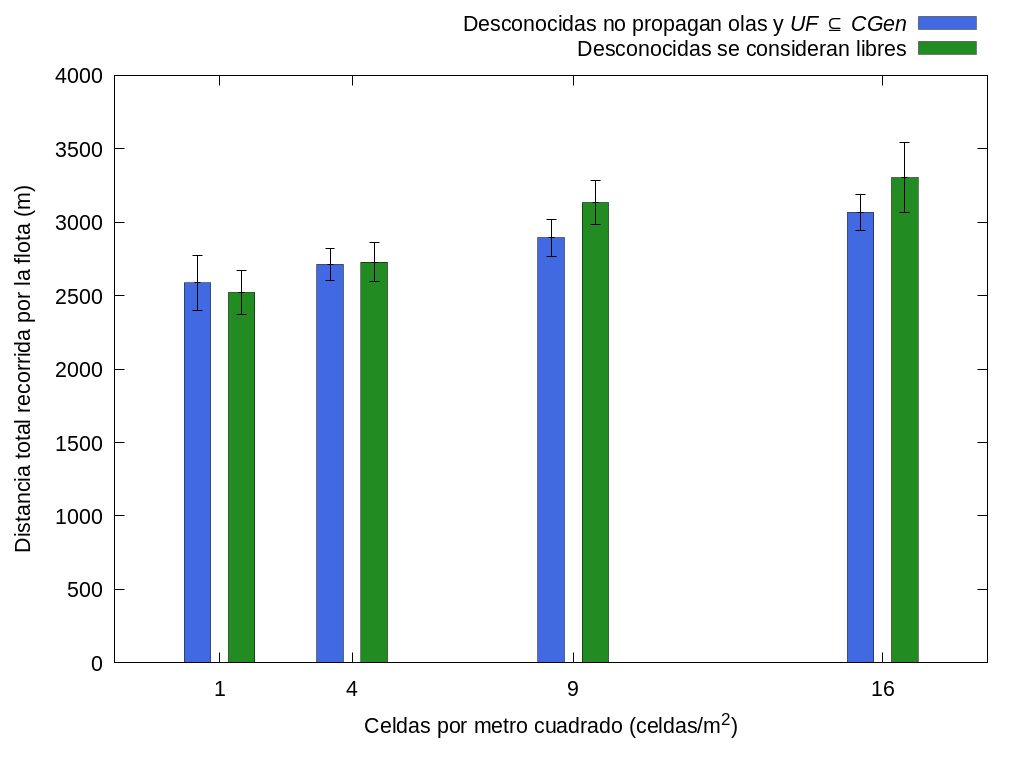
\includegraphics[clip=true, width=\graphlen]{imagenes/graficas_chicas/graficas_histo_num/desconocido/exploration_cost.png}

  \caption{Gráfica de distancia total recorrida por la flota en función de celdas por metro cuadrado.}\label{fig:gra:des:ec}

\end{figure}

\begin{figure}[H]
  \centerfloat

  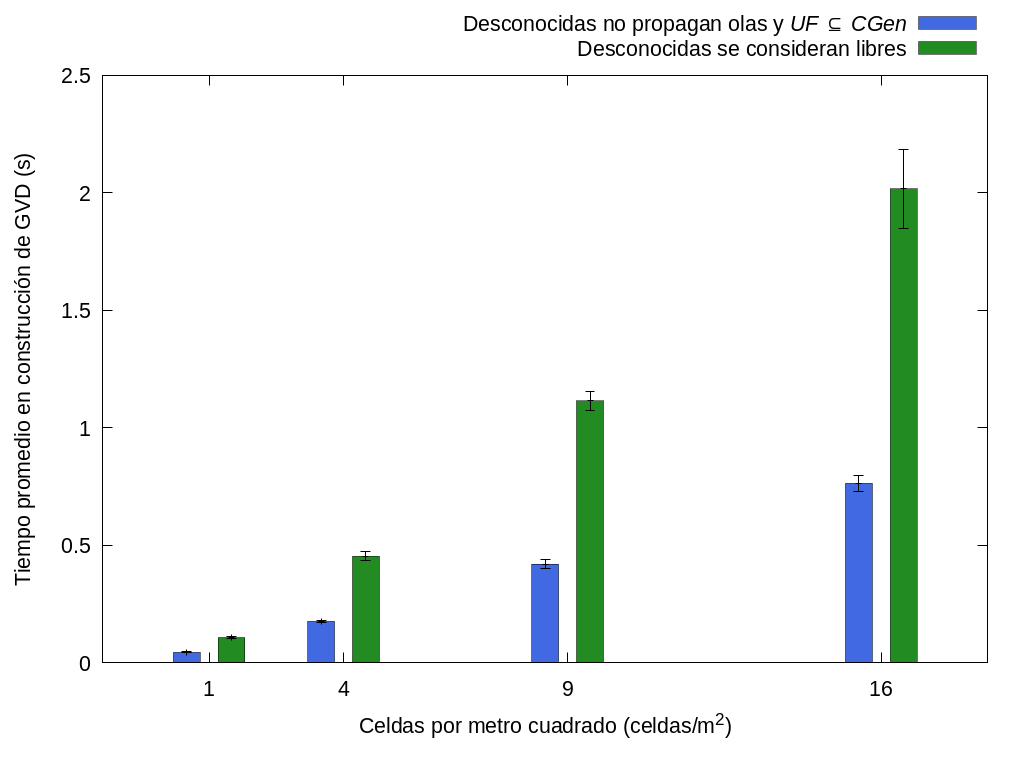
\includegraphics[clip=true, width=\graphlen]{imagenes/graficas_chicas/graficas_histo_num/desconocido/gvd_construction_time_mean.png}

  \caption{Gráfica del tiempo promedio en construcción de GVD en función de celdas por metro cuadrado.}\label{fig:gra:des:gvdt}

\end{figure}

%%%%%%%%%%%%%%%%% ident obj

%%% 1 %%%%
% Es posible apreciar que la variante que identifica como objtivos a las
% fronteras sin simplificar (\emph{FSS}) como objetivos obtiene los peores
% resultados en terminos de tiempos de exploración. Esto explica de forma analoga
% a como se explico el comportamiento de esta misma metrica en la sección
% \ref{sec:exp:inc}. En este caso lo que impacta en el tiempo de la asignación de
% tareas es la la existencia de una cantidad mayor de objetivos que causa que las
% etapas de valuación (sección \ref{subsec:MiValSub}) y de resolución (sección
% \ref{subsec:MiResSub}) tomen más tiempo al ser mayor la cantidad de objtivos a
% valuar y asignar. De los tiempos de exploración obtenidos al utlizar los otros
% dos metodos se deduce que estos consiguen reducir las duraciones de las asignaciónes de
% tareas, cosa que logran invertiendo tiempo en reducir los objetivos
% indentificados al simplificar las fronteras a sus celdas más significativas.
% Especificamente en las pruebas realizadas el simplificar las fronteras reduce
% los tiempos de exploración con respecto a no simplificar, aunque comenzando por
% el nivel más bajo de granularidad la reducción es despreciable esta crece hasta
% alcanzarse una reducción de ${\smallsim}29\%$ en el nivel de granularidad más
% alto.
%%% 2 %%%%
% Es posible apreciar que la variante que identifica como objtivos a las
% fronteras sin simplificar (\emph{FSS}) como objetivos obtiene los peores
% resultados en terminos de tiempos de exploración, o lo que es lo mismo, los
% metodos que simplifican las fronteras reducen los tiempos de exploración con
% respecto a no simplificar. Aunque comenzando por el nivel más bajo de
% granularidad las reducciones son despreciables estas crecen hasta alcanzar una
% reducción de ${\smallsim}29\%$ en el nivel de granularidad más alto. Esto en
% parte se debe a lo explicado en la sección \ref{sec:exp:inc} con respecto a
% esta metrica. En este caso lo que impacta en el tiempo de la asignación de
% tareas es la cantidad de objetivos identificados, ya que aumentar dicha
% cantidad implica aumentos en la duracion de las etapas de valuación (sección
% \ref{subsec:MiValSub}) y de resolución (sección \ref{subsec:MiResSub}) al ser
% mayor la cantidad de objtivos a valuar y asignar. De los tiempos de exploración
% obtenidos al utlizar los otros dos metodos se deduce que estos consiguen
% reducir las duraciones de las asignaciónes de tareas, cosa que logran
% invertiendo tiempo en reducir los objetivos indentificados al simplificar las
% fronteras a sus celdas más significativas.
%%% 3 %%%%
% Es posible apreciar que los metodos que identifican los objetivos simplificando
% las fronteras reducen los tiempos de exploración con respecto al método que
% identifica a las fronteras sin idenficar como obtivos. Aunque en el nivel más
% bajo de granularidad las reducciones son despreciables estas crecen junto a la
% granularidad, hasta alcanzarse una reducción de ${\smallsim}29\%$ en el nivel
% de granularidad más alto. Esto debe en parte a los tiempos de asignación de
% tareas, por lo explicado en la sección \ref{sec:exp:inc} con respecto a esta
% metrica. En este caso el principal impacto en
% los tiempos de asignación de tareas es la cantidad de objetivos identificados.
 
% implica reducciones en la duracion de las etapas de valuación (sección
% \ref{subsec:MiValSub}) y de resolución (sección \ref{subsec:MiResSub}) al ser
% menor la cantidad de objetivos a valuar y asignar. Aunque otra razon posible,
% es que el simplificar las fronteras puede coordinar a los robots. Por ejemplo
% de no simplificarse las fronteras se permite que un robot sea asignado a un
% objetivo adyacentes a una pared o que dos robots sean asignados a objetivos
% adyacentes entre si, situaciones en las cuales se desaprovecha capacidad de
% sensado, y se complejiza la navegacion. Al simplificarse las fronteras,
% especialemente cuando se logra el cubrimiento minimizando los objetivos
% resultantes, se evitan las situaciones descritas similares lo cual puede verse
% como una coordinación implicita.


%%% 4 %%%%
% Los metodos que simplifican las fronteras invierten tiempo en simplificar para disminuir dicha la cantidad de objetivos

% costo computacional vs  
%%, cuando los tiempos de simplificación son los más cortos,
%%

  % Dado que la
% simplificación basada en cubrimiento tiene siempre un mayor costo temporal que
% la basada en K-Means pero logra obtener

% Lo cual implica que el método que simplifica basadose en el cubrimiento tiene
% una inversion mayor de tiempo, y a pesar.
% En este caso ambos metodos invierten tiempo en disminuir los
% objetivos identificados a partir de simplificar las fronteras.

% Con respecto a las dos tecnicas de simplificación estas tienen comportamientos
% similares tanto en el tiempo de exploración como en distancia total recorrida
% por la flota. En el nivel de granularidad más bajo, la simplificación basada en
% cubrimiento logra una reducción con respecto a la basada en K-Means, de
% ${\smallsim}3\%$ de la distancia total recorrida por la flota y de

  % Esto concuerda con lo
% que ocurre en los niveles de granularidad más altos, donde la simplificación
% basada en cubrimiento obtiene peores resultados que la basada en K-Means. Con
% respecto al nivel de granularidad más bajo, lo que puede estar sucediendo es
% que al ser el nivel con menos costo computacional y por lo tanto 

% ste comportamiento en parte se explica por los tiempos de
% asignación de tareas y su efecto en dichas metricas. En este caso aunque pueden
% existir diferencias entre los numeros de objetivos identificados, estas son
% menos significativas repecto a identificar todas las fronteras como objetivos.
% Dado esto para los metodos que simplifican las fronteras se pasa a considerar
% otro factor de impacto de los tiempos de asignación, el tiempo que demora dicha
% simplificación. 

% En este caso ambos
% metodos reducen la cantidad de objetivos identificados simplificando las
% fronteras, por lo tanto aunque pueden existir diferencias entre los numeros de
% objetivos identificados en estos metodos, estas son menores en comparacion al
% todas las fronteras como objetivos, y en consecuencia este aspecto tiene menor
% impacto sobre el tiempo de la asignación de objetivos. Dado esto se pasa a
% considerar otro factor de impacto de los tiempos de asignación: el tiempo que
% demora la simplificación de fronteras. 

% Dado esto se pasa a
% considerar otro factor de impacto de los tiempos de asignación: el tiempo que
% demora la simplificación de fronteras. Según los resultados el tiemp

% Dado que estos metodos
% solo difieren en como realizan la simplificación de fronteras, la demora de
% dicha simplificación es uno de los principales factores a tener en cuenta.



% dado que los tiempos de demora de la asignación de tareas se determino como un
% factor, que aunque tenia un peso, no era significativos, y en este caso donde
% las demoras según los timpos de exploraicon son menores, se obtienen
% diferencias de distancia más significativas entoces, se puede deteminar que la
% coordinación implicita es un factor de impacto en la distnacia.
% La variante \emph{FSS} también obtiene los peores resultados en terminos de
% distancia total recorrida por la flota. Este resultado se atribuye en primer
% lugar a que al ser todas las celdas fronteras objtivos posibles, esto permite asignaciones

% Y en segundo lugar al amuento del tiempo de asignación de tareas como se
% explica en la sección \ref{sec:exp:inc},  



%aunque esto no justifica que las reducciónes de las
% distancias sean mayores a las obtenidas en las pruebas de dicha seccion a pesar de que las 

% simplificandose
% la navegación y aprovechandose las capacidades sensoriales de los robots. Esto

% A simple vista este factor parece contradecir los resultados obtenidos, ya
% que el método que obtiene los peores resultados es el menos impactado por
% este factor ya que no simplifica las fronteras. Lo que sucede es que el
% tiempo de simplificación es en realidad una inversion de tiempo que se hace
% para reducir la cantidad de objetivos

% las simplificaciones que minimizan el numero de fronteras significativas
% mientras mantienendo el cubrimiento minimizan el solapamiento de sensado de
% los robots, aumentado la nueva información que se obiente dele entorno. es la
% principal razon por la cual se introducen los metodos basados en
% simplificación, ya que estos la cantidad de objetivos para disminuir el
% tiempo total de la asignación de tareas.

% se mantienen entre un ${\smallsim}9\%$ y ${\smallsim}11\%$, exceptuando la
% granularidad de una celda por metro cuadrado en la simplificación basada en
% K-Means, en la que se obtiene una reduccion del ${\smallsim}7\%$

% Con respecto a las dos tecnicas de simplificación los comportamientos en las
% metricas de tiempo de exploración y distancia total recorrida por la flota son
% similares.
% , tienen comportamientos similares tanto en el
% tiempo de exploración como en distancia total recorrida por la flota. 
% omo los niveles de granularidad tienen el proposito
% variar la carga computacional, los resutados mencionados parecen indicar que la
% simplificación basada en el cubrimiento es la mejor cuando la carga
% computacional es baja, siendo superada por la simplificación basada en K-Means cuando
% la carga computacional es alta. 

%%%%%%%%% cub y cal
% De la
% equacion 4 se de deduce que el cubrimiento siempre es mayor o igual que la
% calidad. Por lo tanto 


%%%%%%%%
% Dado que las diferencias son despreciables se puede
% concluir que el impacto de el uso de las distintas tambien despreciable.

% confirman que todas las variantes de la implemetnacion 
% finalizar su ejecucion con un mapa casi completo del entorno.

% Estos resutlados son los esperados ya que
% la mision concluye al no quedar más espacio por explorar.

% Es posible apreciar que todos los
% mapas cubren casi en su totalidad al entorno y que la calidad de dichos mapas
% es casi perfecta en todos los casos.



\chapter{Conclusiones y trabajo futuro}\label{cha:concl}
\hfuzz=10pt 
\minitoc
\hfuzz=0pt 

Este proyecto de grado se planteó el objetivo de mejorar la solución del
problema de exploración multi-robot propuesta en \cite{wurm2008coordinated},
donde se propone una estrategia de coordinación para entornos estructurados
que consiste en explorar el entorno maximizando la distribución de los robots sobre las
habitaciones y corredores (segmentos) que se identifican a partir de un
GVD. Para esto se evaluaron varios aspectos de la propuesta en cuestión y del
problema de exploración multi-robot en general relevando una serie de
potenciales mejoras. Estas fueron implementadas como parte de una solución al
problema de exploración multi-robot\footnote{Disponible en línea:\\
\url{https://gitlab.fing.edu.uy/federico.ciuffardi/pgmappingcooperativo}.\\Accedido por última vez: 25/02/2022.} con
la cual se experimentó dentro de un simulador con el propósito de validar su
impacto.

En este ultimó capítulo se plantean las conclusiones derivadas del trabajo
realizado en el proyecto de grado y se establecen líneas de trabajo que pueden ser
continuadas en el futuro.

\section{Conclusiones}

% Este proyecto de grado se planteo como objetivo mejorar la propuesta de
% coordinación para la exploración multi-robot de \cite{wurm2008coordinated} en la
% que se establece que la exploración debe realizase maximizando la distribución
% de los robots sobre las habitaciones y corredores (segmentos), los cuales son
% identificados a partir de un GVD. Para esto se evaluaron varios aspectos de la
% propuesta en cuestión y del problema de exploración multi-robot en general
% relevando una serie de potenciales mejoras. Estas fueron implementadas como
% parte de una solución al problema de exploración multi-robot \footnote{Disponible en línea:\\
% \url{https://gitlab.fing.edu.uy/federico.ciuffardi/pgmappingcooperativo}} con la cual se
% experimento dentro de un simulador con el propósito de validar su impacto.

En general, a partir de los resultados obtenidos en la experimentación, se
concluye que la solución desarrollada resuelve el problema de exploración
multi-robot de forma satisfactoria en términos de los mapas generados. 

Por otro lado se puede concluir que es posible realizar la construcción del GVD
de forma incremental sin perder la información secundaria necesaria para
identificar los segmentos. Es decir, que es posible aplicar la estrategia de
coordinación de \cite{wurm2008coordinated} construyendo el GVD de forma
incremental. Esto se logró adaptando el algoritmo presentado en \cite{Lau2013}
para incluir la información necesaria. A su vez los datos experimentales permiten
concluir que la construcción incremental del GVD acelera significativamente los
tiempos de construcción del GVD y de exploración, frente a realizar una
construcción no incremental como en la propuesta original. Esto es una mejora
considerable en tanto hace viable aplicar la estrategia de coordinación en
entornos de mayor tamaño o que requieran mapas con un mayor nivel de detalle.

% lagf exploración de

También se concluye que el espacio desconocido puede ser considerado de
distintas maneras en la construcción del GVD. En especial que puede considerase
de forma de limitar la construcción del GVD al espacio conocido, lo cual lleva
a una reducción de los tiempos de construcción del GVD y de exploración, con
respecto a realizar la construcción en todo el espacio (conocido y desconocido)
como es usual.

% También se concluye que el espacio desconocido puede ser considerado de
% distintas maneras en la construcción del GVD. En especial que puede considerase de
% forma de limitar la construcción del GVD al espacio conocido, lo cual lleva a
% una reducción de los tiempos de construcción del GVD y de exploración, con
% respecto a realizar la construcción en todo el espacio, como es usual.


% tambien se concluye que al construir el gvd el espacio desconocido puede
% considerase de forma de limitar la construcción al espacio conocido, lo cual
% lleva a una reduccion de los tiempos de construcción del gvd y de
% exploración, con respecto a realizar la construcción en todo el espacio como
% es usual.

En relación a la identificación de objetivos, según los resultados
experimentales se concluye que utilizar todas las fronteras como objetivos
tiene un impacto negativo considerable en los tiempos de exploración y en menor
medida en la distancia que recorren los robots, frente a reducir el número de
objetivos simplificando las fronteras a sus partes más significativas.
Respecto a la simplificación de fronteras se mencionan dos métodos, la
simplificación basada en K-Means que se encuentra presente en el estado del
arte, y la simplificación basada en cubrimiento que es propuesta en este proyecto como
mejora de la anterior. Los resultados experimentales permiten concluir que la
simplificación basada en cubrimiento logra una mayor reducción de objetivos\todo{ya comenté al respecto, ojo!} que
la simplificación basada en K-Means, pero es menos eficiente.\todoremark[inline]{Me quedaba la duda si por eficiencia se daba a entender solo que es mas lento y/o se podia entender que implicaba algo sobre la calidad del resultado | chavacano! es menos eficiente?}
% pero tiene un rendimiento inferior en términos de costo computacional.

Adicionalmente existen dos mejoras potenciales sobre las cuales únicamente se
puede concluir que funcionan correctamente por formar parte de la solución
implementada, pero que su impacto no fue aislado y estudiado experimentalmente.
La primera es el modelo de planificación que combina jerárquicamente la
planificación sobre el GVD, y la planificación sobre todo el espacio libre.
Esta forma de planificar debería implicar reducciones en las distancias
recorridas frente a navegar únicamente sobre el GVD y de costos computacionales
frente a calcular los caminos directamente sobre todo el espacio libre. La
segunda es el algoritmo de asignación de objetivos que fue propuesto como
alterativa al utilizado en el trabajo original de \cite{wurm2008coordinated}.
La principal ventaja de este algoritmo es que logra maximizar la distribución
de los robots sobre los segmentos evitando asignar más robots a un segmento que
los objetivos contenidos en él.

% como si puede
% ocurrir en la propuesta original por asignarse más robots a un segmento que los
% objetivos que se encuentran en él.


% La conclusion principal es que el objetivo se cumplio de forma satisfactoria,
% varias mejoras relacionadas a los aspectos de asignación de tareas, construcción
% del GVD y planificación, fueron presentadas y validadas con la solución
% dearrollada. 

% Las mejoras estan asociadas construcción del GVD y identificación de objetivos.

% La principal mejora consiste en hacer uso de un algoritmo incremental para
% contruccion del GVD en lugar de uno no incremental como en la propuesta
% original.

% el desarrollo una solucion al problema de
% exploración multi-robot basada en \cite{wurm2008coordinated} 

% Uno de
% los aspectos principales de la exploración multi-robot 

% En este proyecto se trabajo sobre el problema de exploración multi-robot. 

% En este proyecto se describio y 

% Varios aspectos de la exploración
% multi-robot fueron analizados derivando en propuestas 

% La solucion desarrollada a

% \todo[inline]{seguir con las dos mejoras, ir mezclando las conclusiones de las pruebas capaz.}

% El trabajo desarrollado trata sobre el problema de exploración utilizando un
% grupo de robots, más específicamente sobre como lograr distribución eficiente
% de los robots en el espacio para una mayor coordinación en la exploración. Para
% esto, en lugar de distribuir los robots sobre las fronteras entre el espacio
% conocido y el desconocido, como es usual, la propuesta apunta a identificar
% porciones del espacio similares a habitaciones o corredores, llamados
% segmentos, para luego distribuir los robots primero sobre dichos segmentos y
% luego sobre las fronteras de los mismos.

% punteo
% * La exploración es un problema complejo:
%   * involucr varios subprobleaas de la robtica que deben interactuar entre si para lograr
% * La

\section{Trabajo a futuro}

Esta sección se dedica a comentar las líneas de trabajo que surgen del proyecto
realizado y pueden ser retomadas a futuro.

\subsection{Experimentación en la realidad}

Una de estas líneas de trabajo es la de realizar experimentos en la realidad \todoerror[inline]{No se entiende que se quiere decir con experimentos en la realidad? O es para hacerlo explicito? Digo porque el titulo de la subsection es así y en la presentación lo tengo así también | con una flota de robots reales?}
con el propósito de validar los resultados obtenidos en los experimentos
simulados. Esto no es una tarea trivial ya que, además de requerirse hardware y
un entorno en donde hacer las pruebas, también se deben remover las hipótesis de
comunicación y localización ideales de los robots\todoerror[inline]{Era para fundamentar el porque se relaciona con experimentar en la realidad, lo saco igual? | sacar lo que sigue.}, dado que estas
no son viables en la realidad. Esto hace necesario alterar la
implementación de forma que los potenciales problemas de comunicación
sean considerados y evitados durante la exploración \cite{amigoni2017multirobot}. Y por otro lado requiere
integrar una solución de localización que permita estimar la ubicación de los
robots \cite{slam}. % en un escenario real.

\subsection{Identificación de objetivos}
% esta relacionada al
% método de identificación de objetivos que funciona simplificando fronteras
% basándose en el cubrimiento. Como se comento en la secón de conclusiones,
% dicho método obtiene una reducción de objetivos mejo

% posibilidad de mejorar el rendimiento computacional del 

También se abren dos líneas de trabajo que profundizan en el estudio y
desarrollo de métodos de identificación de objetivos. La primera está orientada
al análisis del método de simplificación de fronteras basado en el cubrimiento
en busca de posibles optimizaciones que logren mejorar su rendimiento
computacional, que actualmente es su mayor desventaja. La segunda consiste en
el desarrollo de variantes del método antes mencionado, que en lugar de
determinar de forma arbitraria cual frontera es la significativa del conjunto
de candidatas, se determine con algún criterio específico, como por ejemplo elegir la
frontera candidata con mayor ganancia de información \cite{Amorin2019}.

% La tercera es
% el estudio de otros métodos identificación de objetivos, como por ejemplo la simplificación.

De seguir alguna de estas direcciones también sería conveniente diseñar nuevas
pruebas que se concentren en evaluar la identificación de objetivos, ya que por
ejemplo en el entorno utilizado la mayoría de habitaciones son pequeñas y no son
propensas a generar fronteras con una complejidad suficiente como para
presentar un desafió a los métodos de simplificación estudiados.

 % analizar la posibilidad de optimizar 

% Como se comento en la sección de conclusiones,
% dicho método obtiene una reducción de objetivos mejo

% Comentar que el entorno en el que se realizan las pruebas pone a prueba los
% algoritmos de simplificación principalmente en la habitación grande del centro,
% siendo las demás demasiado pequeñas como para favorecer que se generen
% fronteras con las condiciones de ser largas y serpentean tes, de forma de
% generar las condiciones necesaria para que la simplificación de K-Means
% funcione peor. Quizás el generar un conjunto distinto de pruebas viene bien
% junto a hacerlo más eficiente y también compara contra affinity propagation

% Cuidado con la simplificación de fronteras y los obstáculos que pueden llegar a
% ocluir las fronteras (modificar la def de cubrimiento para que no permita
% oclusiones)



\subsection{Mapa topológico}

En la solución desarrollada la extensión de los segmentos es la única
información necesaria y que se tiene disponible relacionada al mapa topológico.
Por lo que una dirección de trabajo posible sería la de desarrollar un método
para procesar dicha información con el propósito obtener un mapa topológico
completo, como por ejemplo un grafo que contenga un vértice por segmento y las
aristas entre dichos vértices implique la adyacencia entre los segmentos.

Evaluar los mapas topológicos generados a partir de la solución desarrollada
con las ideas presentadas en la sección \ref{sec:evalTop} también se presenta
como una línea de trabajo interesante. Al igual que el estudio, implementación
y validación de técnicas que proponen mejorar la segmentación como las que se
describen en \cite{Thrun1998,wurm2008coordinated,Liu2015}.

% * Mejorar la segmentación, por ejemplo con:
%   * Trun y su mergo de segmentos 
%   * lo descrito en lie Ming y siege wart spectral clustering

% * Evaluar la segmentación incremental con lo mencionado en la sección de criterios del "estado del arte"

% * Hacer la técnica de filtrado de puntos críticos de warm (la de vecino de grado 3) de forma incremental


% tiene consiste de sus segmentos sueltas y el GVD que
%     permite navegar entre estas.
%     * no es necesaria otra para lo que hice pero estaría bueno como herramienta
%       generar un verdadero mapa topológico

% Aoque en la solución del proyecto desarrollado se identifican los segmentos del entorno

% es la de probar distintas formas de segmentación, estudiar el impacto de cada 
% * Consolidar una la generación un mapa topológico verdadero:
%   * ahora el mapa topológico se compone de regiones sueltas y el GVD que
%     permite navegar entre estas.
%     * no es necesaria otra para lo que hice pero estaría bueno como herramienta
%       generar un verdadero mapa topológico
%   * La idea sería reducir los segmentos vertices ubicándoos en sus centros de
%     masa y las conexiones entre ellos (a través del GVD/mapa métrico) a aristas
%     punto a punto entre dichos vertices.


\subsection[Algoritmo de asignación de objetivos y Planificación]{Algoritmo de asignación de objetivos y\\ Planificación}

Otra posible dirección de trabajo que puede ser retomada a futuro es la de
realizar pruebas que permitan comprobar el impacto del algoritmo de asignación
de objetivos introducido en este proyecto, comparándolo contra con otros algoritmos de
asignación de objetivos, como por ejemplo el método húngaro como es utilizado
en \cite{wurm2008coordinated}.

De forma similar otro trabajo futuro posible es el de validar el impacto de la
planificación jerárquica presentada en este proyecto comparándola con otras
estrategias alterativas de planificación. 

\subsection{Potenciales mejoras de rendimiento}

% varios trabajos a futuro que se .. .de esto

Existen varias mejoras potenciales de rendimiento que pueden ser estudiadas,
implementadas y validadas como trabajo futuro. A continuación se presentan
algunos ejemplos.

Un ejemplo sería el paralelizar la segmentación y la identificación de
objetivos en la etapa de obtención de información.

Otro ejemplo consiste en cambiar el algoritmo de segmentación no incremental por una variante
incremental de este, como la presentada en \cite{Liu2015}. 

Los algoritmos de simplificación de frontera son no incrementales y cambiarlos
por variantes incrementales también es un un ejemplo. Aunque en este caso no se
encontró información al respecto por lo que se debería estudiar si esto es
posible.

% Ver posibilidades de un filtrado de fronteras (obtener fronteras significativas) de forma incremental


\subsection{Reusabilidad}

Otro trabajo futuro posible es el de refactorizar, organizar y documentar cada
módulo de la solución desarrollada, con el propósito de proporcionar dichos
módulos como nodos de \gls{ROS} independientes, que sigan los estándares propuestos
por la comunidad de dicha herramienta. De esta forma se facilita la
reutilización de lo desarrollado en este proyecto permitiendo
alcanzar a más investigadores y estudiantes.

Modificar la solución actual que utiliza la primera versión de \gls{ROS} (\gls{ROS} 1)
para utilizar en su lugar a su segunda versión (\gls{ROS} 2), puede ser otra línea de
trabajo de interés pensando en la reusabilidad a futuro, ya que \gls{ROS} 1 termina
su soporte en el 2025.

% * Hacer librerias con los timpos de datos utliados y algormios desarrollados (agnositcos de \gls{ROS} 1)
%   * Esto se hizo (no sería trabajo futuro)

% * Hacer paquetes de \gls{ROS} 1 que sigan los estandares, sean modulares y resutilizables 
%   * Ahora esta todo junto dentro de un paquete pero los modulos son
%     relativametne independientes entre si y podrian modularizarse para su
%     reutlizacion y combinacion con otros paquetes


% * Hacer lo mismo del punto anterior con ros2:
%   * Discutir que esto es lo más razonable ya que:
%     * \gls{ROS} 1 termna su soporte pronto
%     * \gls{ROS} 2 es ampliamente superior cuando se trata de multi-robot (no es centralizado)

% \subsection{Remocion de hipotesis}

% X Se podria trabajar para remover la hipotesis de comunicacion ideal, esto introduce el desafio de considerar los kkkkk

% X comunicacion ahora es ideal, si quisieramos simular mejores comuniciaiones nosotros deberiamos investigar co-simulacion (simulador de fisicas gazebo y simulador dee redes).
%     * Ver de comentar cocosim

% X ubiacion ahora es ideal podria ver que desafios introduce el uso la remocion de esta restriccion


% * Hipotesis de saber las dimenciones del mapa estaria buena removerla , dar ideas

% * Hay que comentar homogeneidad como restriccion que estamos tomando:
%   * Ahora las fronteras accesibles en la grilla son accesibles por todos los robots 
%     * Por ser homogeneos y cierculares los robots se puede engordar los obstaculos por el radio del robot y eso asegura lo del punto antesrior.
%   * De lo contrario si los tamanio 
%   * tipos de fronteras dependiendo de la accesibilidad : de percepcion y de movilidad
%     * se podria asignar dimendsiones mínimas de lso robots a las fronteras (para un camino tengo los vertices y cada uno tiene distancia mínima a los obstaculos entoces la mínima distancia a un obstaculo es tu dimencion máxima si no te vas a chochar). 


%   * Por ahora los entornos se considerarn estaticos, y en mayor parte lo son (solo los demas robots son dinamicos). Levantar esta restriccion tambien es un trabajo a futuro interesante. Ver de modelar puertas personas , etc y como manejarlas. Puertas como cosas que se pueden abrir. Personas como cosas a esquivar pero que no queneran segmentos etc.




\begin{appendices}
\chapter{Algoritmos completos}

\section{Obtención de celdas base}\label{algComp:celdasbase}
El algoritmo \ref{alg:celdasBaseCompleto} es una versión del algoritmo \ref{alg:celdasBase} sin las
simplificaciones comentadas en la sección \ref{subsec:critPer}.

\begin{algorithm}[H]
\SetAlgoLined
  \SetKwInOut{Input}{Entrada}
  \Input{$c$}

% En updateBase c es pN y cA es p
% En setPseudoSourcesFromWave c es p y cA es waveP
  % \tcp{DFS desde $c$ agregando las celdas visitadas a la componente conexa $C_i$}
  $\mli{CB}_c := \emptyset$

  \ForEach{ $cA \in ady(c)$} {
    \ForEach{$b \in gens(cA)$} {
      $\mli{tolerado}  := d_c(b) \leq \mli{DD}(c) + L$\\
      % $\mli{noIgNiAdy} := b \notin gens(c) \land b \notin \bigcup_{b'} ady(gen(c))$\\

      $\mli{masCercano} := verdadero$\\
      $\mli{aRemover} := \emptyset$\\
      % \ForEach{$b' \in \mli{CB}_c$ \textbf{mientras} masCercano } {
      \ForEach{$b' \in \mli{CB}_c$} {
        \If{$b' = b \lor b' \in ady(b)$}{
          \uIf{$d_c(b) < d_c(b')$}{
            $\mli{aRemover} := \mli{aRemover} \cup \{b'\}$\\
          }\Else{
            $\mli{masCercano} := \mli{masCercano} \land falso$ \\
            \tcp{No es necesario continuar con la iteración de la línea 7 una vez ejecutada esta línea}
          }
        }
      }
      
      \If{tolerado $\land$ masCercano}{
        $\mli{CB}_c := \mli{CB}_c -\mli{aRemover}$\\
        $\mli{CB}_c := \mli{CB}_c \cup \{\mli{b}\}$\\
      }
    }
  }
  \Return $\mli{CB}_c$ 

  \caption{Obtención de las celdas base $\mli{CB}_c$ de una celda $c$}
  \label{alg:celdasBaseCompleto}
\end{algorithm}

\newpage
Uno de los principales cambios respecto al algoritmo \ref{alg:celdasBase} es el
remplazo de la función $gen$ por la función $gens : \mli{CG} \rightarrow
P(\mli{CGen})$ que dada una celda $c$ de la grilla devuelve el conjunto de
todas las celdas que pertenecen a un generador que están a mínima distancia de
$c$. Otro cambio a notar es que la condición asociada a la variable
$\mli{masCercano}$ (líneas 5-15) pasa a ser que la celda base candidata $b$
esté a menor distancia de $c$ que las celdas base actuales $b'$ que son
iguales o adyacentes a $b$. El último cambio a destacar es que la condición que
en algoritmo \ref{alg:celdasBase} se controla con la variable
$\mli{noIgNiAdy}$, en este algoritmo se controla a partir las variables
$\mli{masCercano}$ y $\mli{aRemover}$.
% en la condición
% asociada a la variable $\mli{masCercano}$
% y de cumplirse todas las
% condiciones los $b'$ adyacentes a $b$ dejan de ser celdas base de $c$.
\newpage

\chapter{Ejemplos completos}
\begingroup
\small
\section{Simplificación de fronteras basada en cubrimiento}\label{EXE:sfbc}
La figura \ref{EXE:sfbc} presenta la versión completa del ejemplo mostrado en la figura \ref{fig:ejemploFSCub}.
\endgroup
\begin{figure}[H]
  \centerfloat
  \subfloat[Estado inicial.]{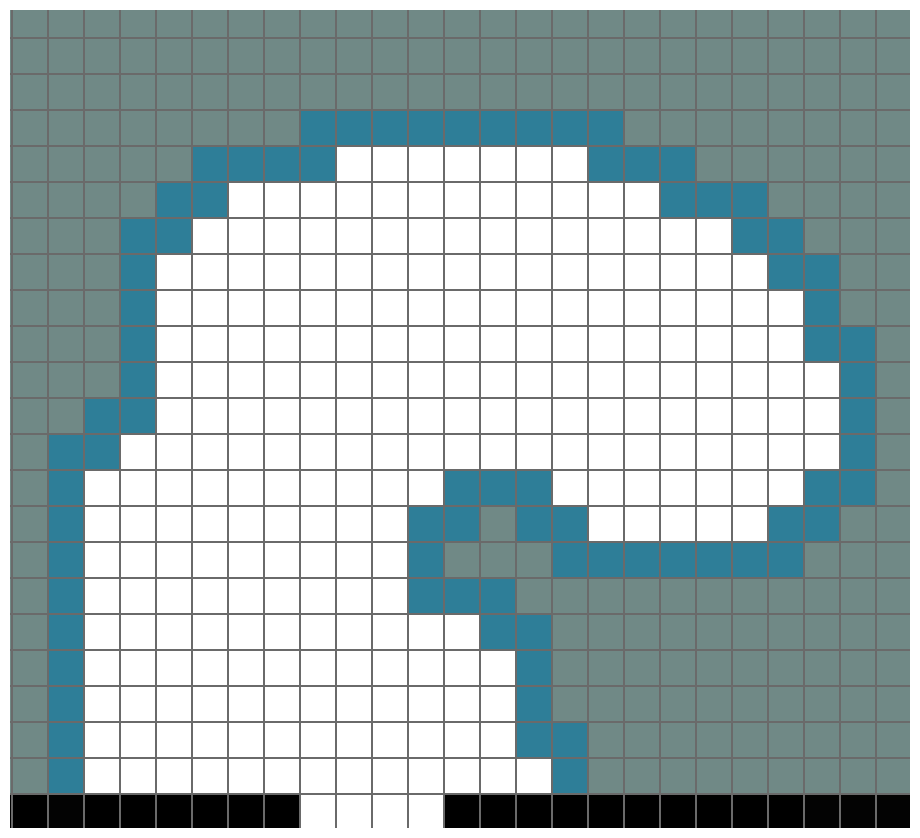
\includegraphics[clip=true, width=0.48\textwidth]{imagenes/ejemploSimpCub/a1.png}}
  \subfloat[Se inicializa $\mli{FP}$.]{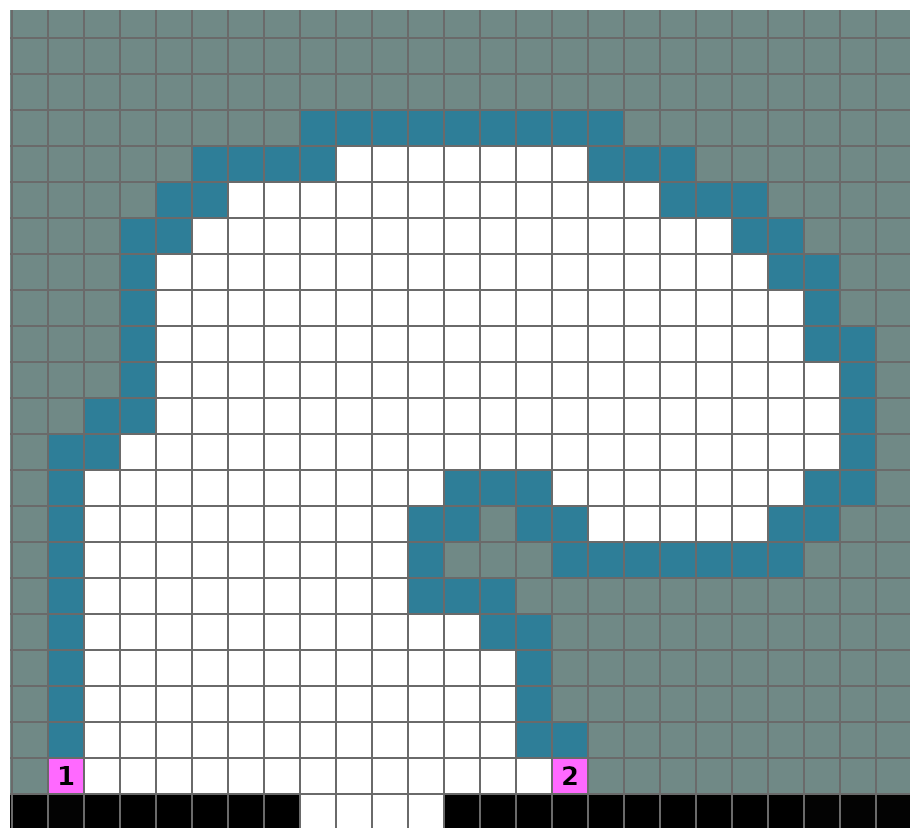
\includegraphics[clip=true, width=0.48\textwidth]{imagenes/ejemploSimpCub/a2.png}}

  \subfloat[Se obtiene $\mli{fp}$ desencolando de $\mli{FP}$.]{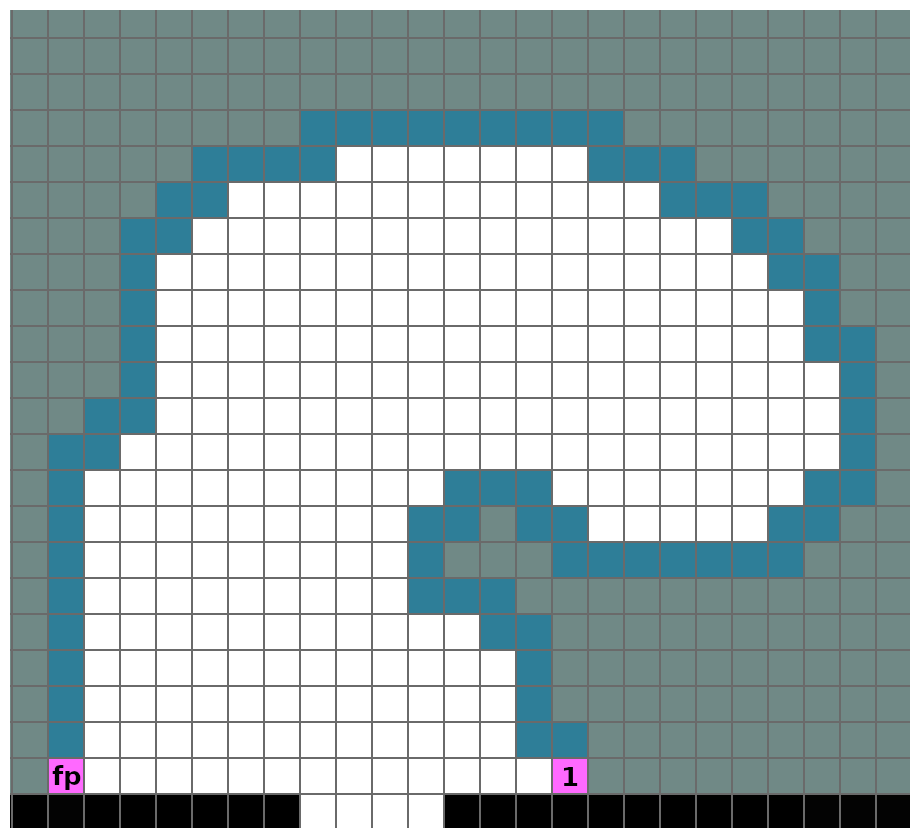
\includegraphics[clip=true, width=0.40\textwidth]{imagenes/ejemploSimpCub/b1.png}}
  \subfloat[Existen celdas en $\mli{UF}$ a una distancia mayor que $2*rango$ de $\mli{fp}$, los candidatos se obtienen con $radio=rango$. ]{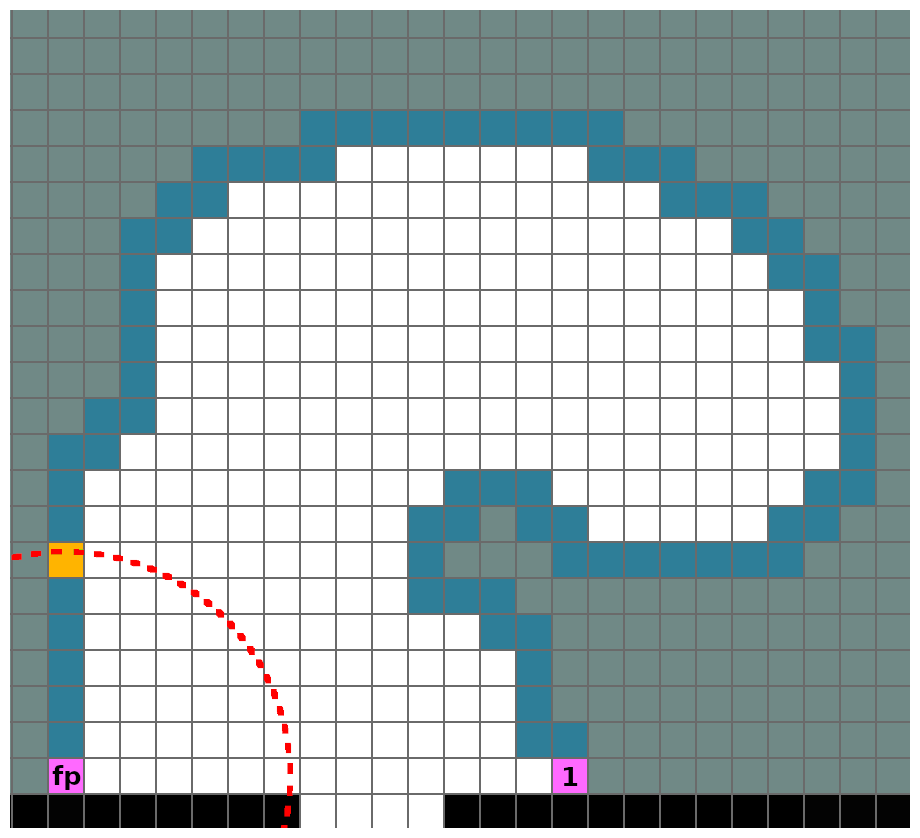
\includegraphics[clip=true, width=0.40\textwidth]{imagenes/ejemploSimpCub/b3.png}}
  \subfloat[Se elige el único candidato como $\mli{fs}$, se actualiza $\mli{UF}$, $\mli{FS_i}$ y $\mli{FP}$.]{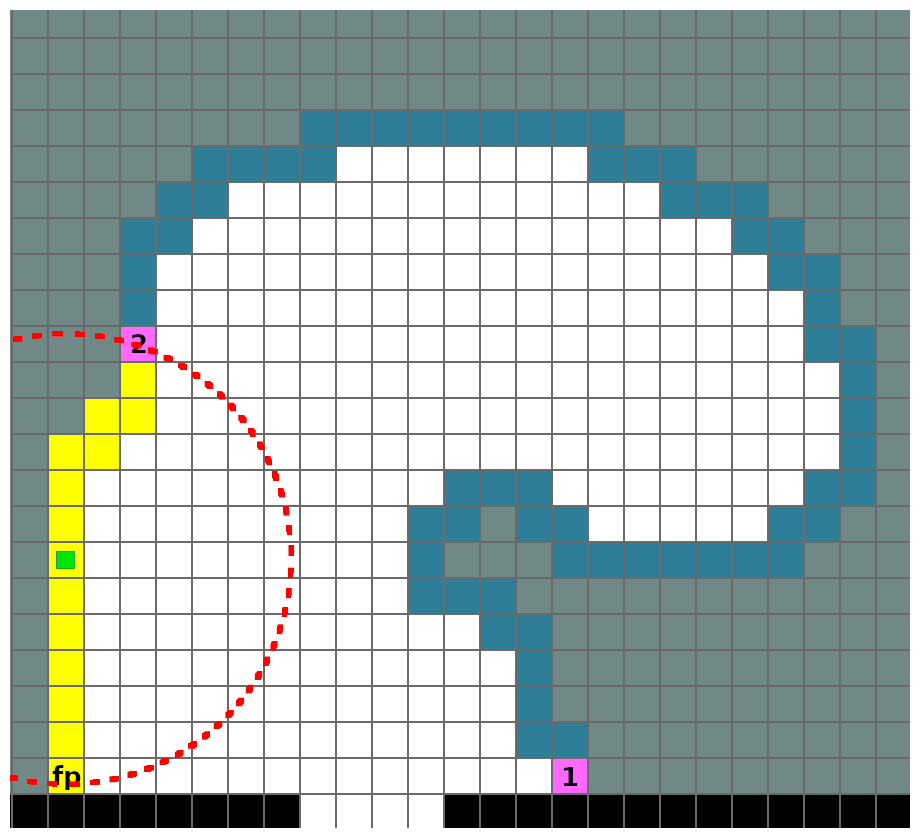
\includegraphics[clip=true, width=0.40\textwidth]{imagenes/ejemploSimpCub/b5.png}}

 \phantomcaption

\end{figure}

\begin{figure}[H]
  \setcounter{subfigure}{5}
  \centerfloat

  \subfloat[Se obtiene $\mli{fp}$ desencolando de $\mli{FP}$.]{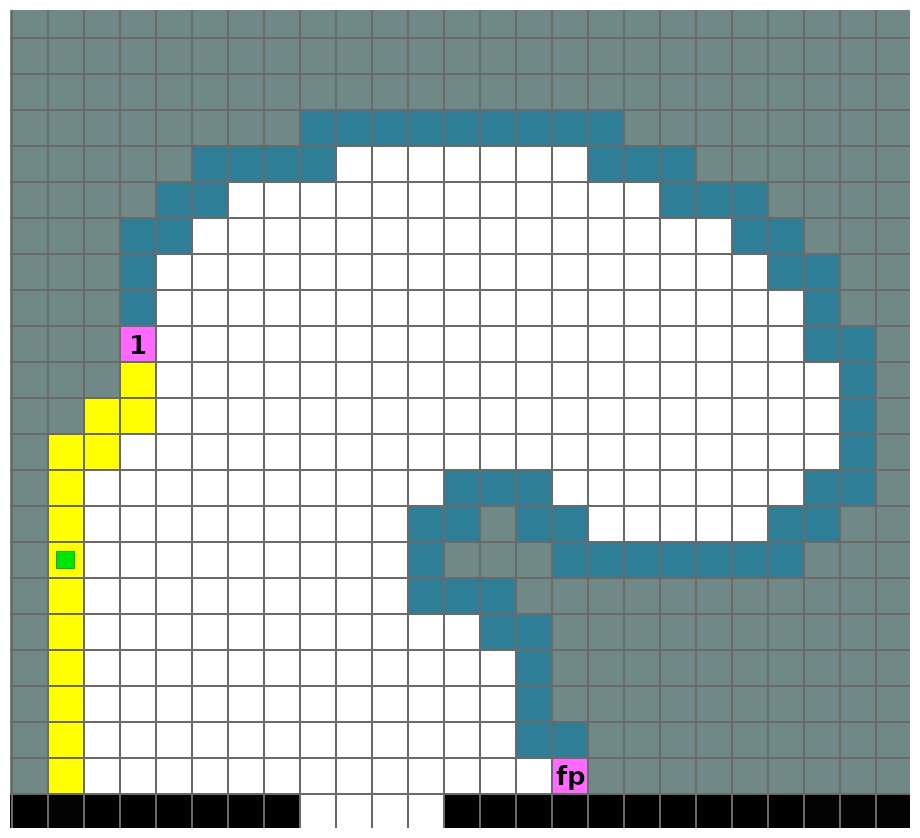
\includegraphics[clip=true, width=0.40\textwidth]{imagenes/ejemploSimpCub/c1.png}}
  \subfloat[Existen celdas en $\mli{UF}$ a una distancia mayor que $2*rango$ de $\mli{fp}$, los candidatos se obtienen con $radio=rango$. ]{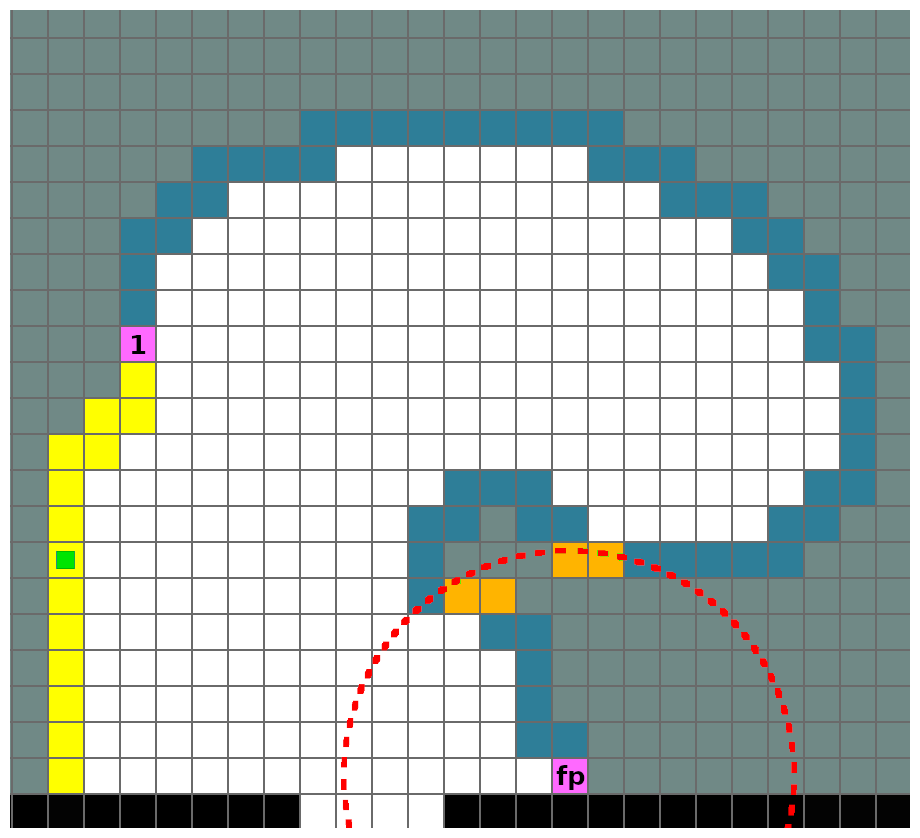
\includegraphics[clip=true, width=0.40\textwidth]{imagenes/ejemploSimpCub/c3.png}}
  \subfloat[Se elige arbitrariamente un candidato como $\mli{fs}$, se actualiza $\mli{UF}$, $\mli{FS_i}$ y $\mli{FP}$.]{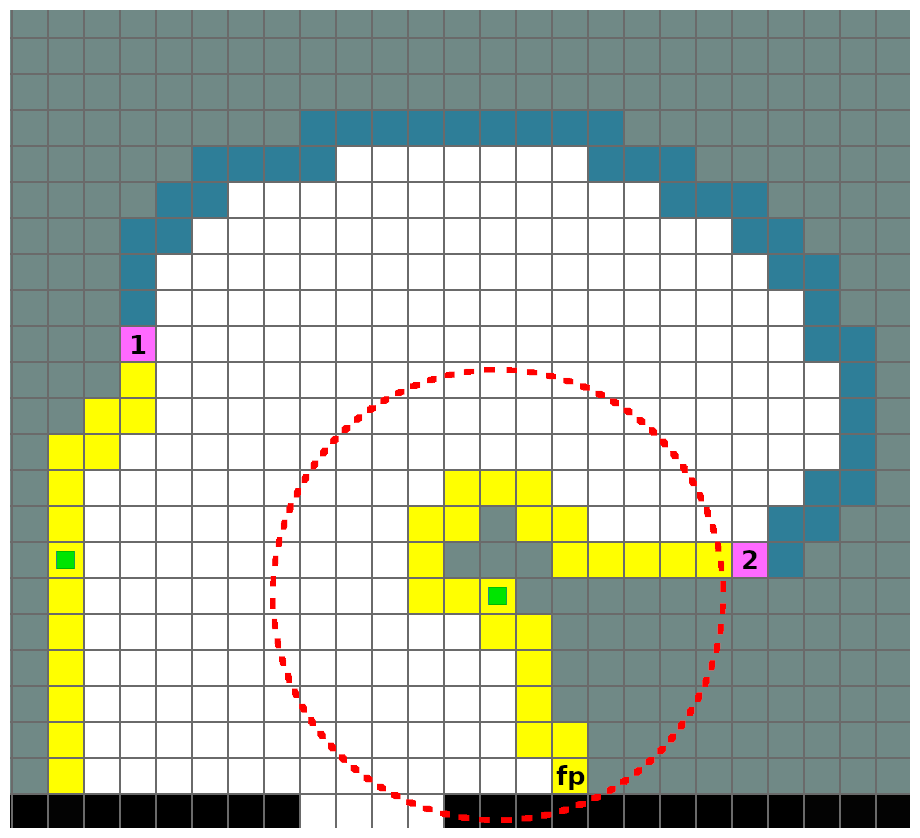
\includegraphics[clip=true, width=0.40\textwidth]{imagenes/ejemploSimpCub/c5.png}}


  \subfloat[Se obtiene $\mli{fp}$ desencolando de $\mli{FP}$.]{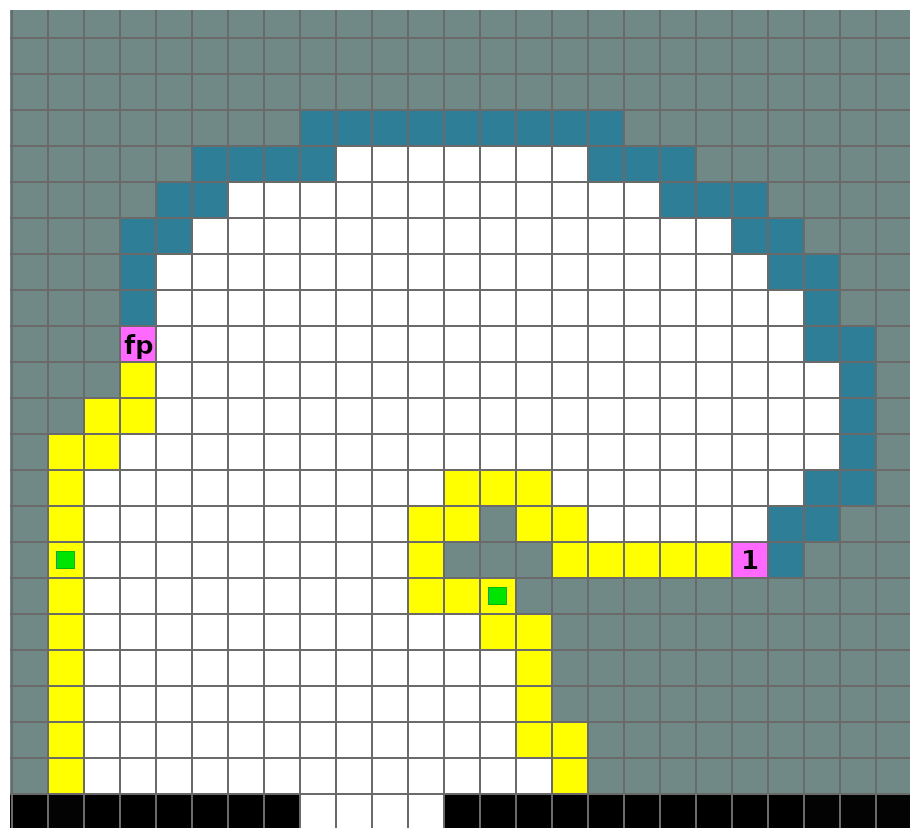
\includegraphics[clip=true, width=0.40\textwidth]{imagenes/ejemploSimpCub/d1.png}}
  \subfloat[Existen celdas en $\mli{UF}$ a una distancia mayor que $2*rango$ de $\mli{fp}$, los candidatos se obtienen con $radio=rango$. ]{\includegraphics[clip=true, width=0.40\textwidth]{imagenes/ejemploSimpCub/d3.png}}
  \subfloat[Se elige arbitrariamente un candidato como $\mli{fs}$, se actualiza $\mli{UF}$, $\mli{FS_i}$ y $\mli{FP}$.]{\includegraphics[clip=true, width=0.40\textwidth]{imagenes/ejemploSimpCub/d5.png}}

  \subfloat[Se obtiene $\mli{fp}$ desencolando de $\mli{FP}$.]{\includegraphics[clip=true, width=0.40\textwidth]{imagenes/ejemploSimpCub/e1.png}}
  \subfloat[Existen celdas en $\mli{UF}$ a una distancia mayor que $2*rango$ de $\mli{fp}$, los candidatos se obtienen con $radio=rango$. ]{\includegraphics[clip=true, width=0.40\textwidth]{imagenes/ejemploSimpCub/e3.png}}
  \subfloat[Se elige el único candidato como $\mli{fs}$, se actualiza $\mli{UF}$, $\mli{FS_i}$ y $\mli{FP}$.]{\includegraphics[clip=true, width=0.40\textwidth]{imagenes/ejemploSimpCub/e5.png}}


 \phantomcaption
\end{figure}

\setcounter{figure}{0}

\begin{figure}[H]
  \setcounter{subfigure}{14}
  \centerfloat

  \subfloat[Se obtiene $\mli{fp}$ desencolando de $\mli{FP}$.]{\includegraphics[clip=true, width=0.40\textwidth]{imagenes/ejemploSimpCub/f1.png}}
  \subfloat[No existen celdas en $\mli{UF}$ a una distancia mayor que $2*rango$ de $\mli{fp}$, la celda de $\mli{UF}$ más alejada está a $\smallsim7.4$ (largos de celda), los candidatos se obtienen con $radio\cong3.7$ (largos de celda). ]{\includegraphics[clip=true, width=0.40\textwidth]{imagenes/ejemploSimpCub/f3.png}}
  \subfloat[Se elige el único candidato como $\mli{fs}$, se actualiza $\mli{UF}$, $\mli{FS_i}$ y $\mli{FP}$.]{\includegraphics[clip=true, width=0.40\textwidth]{imagenes/ejemploSimpCub/f4.png}}


  \subfloat[$\mli{UF}=\emptyset$ por lo que el algoritmo finaliza.]{\includegraphics[clip=true, width=0.40\textwidth]{imagenes/ejemploSimpCub/zfinal1.png}}
  \subfloat[Se logra el cubrimiento.]{\includegraphics[clip=true, width=0.40\textwidth]{imagenes/ejemploSimpCub/zfinal2.png}}
  % \subfloat[$\mli{UF}=\emptyset$ por lo que el algoritmo finaliza.]{\includegraphics[clip=true, width=0.40\textwidth]{imagenes/ejemploSimpCub/zfinal3.png}}

  \caption[Proceso de simplificación de fronteras según cubrimiento.]{Proceso
    de simplificación de fronteras según cubrimiento. Las fronteras de $F_i$ se
    indican con azul si pertenecen a $\mli{UF}$ y con amarillo de lo contrario.
    Con magenta se indican las celdas en $\mli{FP}$ siendo la numeración su
    orden en la cola y $\mli{fp}$ la última desencolada. Las
    circunferencias rojas centradas en $\mli{fp}$ tienen como radio la distancia
    utilizada para obtener los candidatos $\mli{FSC}$ los cuales se indican con
    naranja. Las fronteras significativas se indican con verde, siendo las
    circunferencias rojas de radio $rango=5.6$ (largos de celda) centradas en estas indicadores de su
  cubrimiento.}\label{fig:ejemploFSCubComp}

\end{figure}

\end{appendices}

% == BIBLOGRAPHY ==
\hbadness=10000
%\begingroup
%\bibliographystyle{IEEEtran}   %facundo
\bibliographystyle{apalike}    %facundo
%\raggedright

\bibliography{references}

\end{document}
